%definira klasu dokumenta 
\documentclass[12pt]{report} 

%prostor izmedu naredbi \documentclass i \begin{document} se zove uvod. U njemu se nalaze naredbe koje se odnose na cijeli dokument

%osnovni LaTex ne može riješiti sve probleme, pa se koriste različiti paketi koji olakšavaju izradu željenog dokumenta
\usepackage[croatian]{babel} 
\usepackage{amssymb}
\usepackage{amsmath}
\usepackage{txfonts}
\usepackage{mathdots}
\usepackage{titlesec}
\usepackage{array}
\usepackage{lastpage}
\usepackage{etoolbox}
\usepackage{tabularray}
\usepackage{color, colortbl}
\usepackage{adjustbox}
\usepackage{geometry}
\usepackage[classicReIm]{kpfonts}
\usepackage{hyperref}
\usepackage{fancyhdr}

\usepackage{float}
\usepackage{setspace}
\restylefloat{table}


\patchcmd{\chapter}{\thispagestyle{plain}}{\thispagestyle{fancy}}{}{} %redefiniranje stila stranice u paketu fancyhdr

%oblik naslova poglavlja
\titleformat{\chapter}{\normalfont\huge\bfseries}{\thechapter.}{20pt}{\Huge}
\titlespacing{\chapter}{0pt}{0pt}{40pt}


\linespread{1.3} %razmak između redaka

\geometry{a4paper, left=1in, top=1in,}  %oblik stranice

\hypersetup{ colorlinks, citecolor=black, filecolor=black, linkcolor=black,	urlcolor=black }   %izgled poveznice


%prored smanjen između redaka u nabrajanjima i popisima
\newenvironment{packed_enum}{
	\begin{enumerate}
		\setlength{\itemsep}{0pt}
		\setlength{\parskip}{0pt}
		\setlength{\parsep}{0pt}
	}{\end{enumerate}}

\newenvironment{packed_item}{
	\begin{itemize}
		\setlength{\itemsep}{0pt}
		\setlength{\parskip}{0pt}
		\setlength{\parsep}{0pt}
	}{\end{itemize}}




%boja za privatni i udaljeni kljuc u tablicama
\definecolor{LightBlue}{rgb}{0.9,0.9,1}
\definecolor{LightGreen}{rgb}{0.9,1,0.9}

%Promjena teksta za dugačke tablice
\DefTblrTemplate{contfoot-text}{normal}{Nastavljeno na idućoj stranici}
\SetTblrTemplate{contfoot-text}{normal}
\DefTblrTemplate{conthead-text}{normal}{(Nastavljeno)}
\SetTblrTemplate{conthead-text}{normal}
\DefTblrTemplate{middlehead,lasthead}{normal}{Nastavljeno od prethodne stranice}
\SetTblrTemplate{middlehead,lasthead}{normal}

%podesavanje zaglavlja i podnožja

\pagestyle{fancy}
\lhead{Programsko inženjerstvo}
\rhead{Medicinska rehabilitacija}
\lfoot{Seven Smurfs}
\cfoot{stranica \thepage/\pageref{LastPage}}
\rfoot{\today}
\renewcommand{\headrulewidth}{0.2pt}
\renewcommand{\footrulewidth}{0.2pt}


\begin{document} 
	
	
	
	\begin{titlepage}
		\begin{center}
			\vspace*{\stretch{1.0}} %u kombinaciji s ostalim \vspace naredbama definira razmak između redaka teksta
			\LARGE Programsko inženjerstvo\\
			\large Ak. god. 2023./2024.\\
			
			\vspace*{\stretch{3.0}}
			
			\huge Medicinska rehabilitacija\\
			\Large Dokumentacija, Rev. \textit{2}\\
			
			\vspace*{\stretch{12.0}}
			\normalsize
			Grupa: \textit{Seven Smurfs}\\
			Voditelj: \textit{Dora Kašik}\\
			
			
			\vspace*{\stretch{1.0}}
			Datum predaje: \textit{19. 1. 2024.}\\
	
			\vspace*{\stretch{4.0}}
			
			Nastavnik: \textit{Miljenko Krhen}\\
		
		\end{center}

	
	\end{titlepage}

	
	\tableofcontents


	\chapter{Dnevnik promjena dokumentacije}
		
				
		
		\begin{longtblr}[
				label=none
			]{
				width = \textwidth, 
				colspec={|X[2]|X[13]|X[3]|X[3]|}, 
				rowhead = 1
			}
			\hline
			\textbf{Rev.}	& \textbf{Opis promjene/dodatka} & \textbf{Autori} & \textbf{Datum}\\[3pt] \hline
			1.1 & Napravljen predložak	& Marko Miletić & 17.10.2023. 		\\[3pt] \hline 
			1.2	& Dodani opis projektnog zadatka i
funkcionalni zahtjevi & Marko Miletić & 21.10.2023. 	\\[3pt] \hline 
			1.3 & Kreiran dijagram arhitekture & Josip Begić & 22.10.2023. \\[3pt] \hline 
			1.4 & Početak rada na opisu baze podataka & Marko Miletić & 27.10.2023. \\[3pt] \hline 
			1.5 & Dodani opisi tablica baze podataka & Marko Miletić & 02.11.2023. \\[3pt] \hline 
			1.6 & Ažuriran dnevnik sastajanja & Marko Miletić & 09.11.2023. \\[3pt] \hline 
			1.7 & Ažurirana tablica aktivnosti & Marko Miletić & 09.11.2023. \\[3pt] \hline 
			1.8 & Kreiran dijagram baze podataka & Josip Begić & 10.11.2023. \\[3pt] \hline 
			1.9 & Kreiran dijagram komponenti & Josip Begić & 10.11.2023. \\[3pt] \hline 
			1.10 & Kreirani dijagrami razreda & Anton Vivoda & 13.11.2023. \\[3pt] \hline 
			1.11 & Dodani funkcionalni i ostali zahtjevi & Dora Kašik, Katarina Mikulić & 14.11.2023. \\[3pt] \hline
			1.12 & Kreirani sekvencijski dijagrami i dijagrami obrazaca uporabe & Dora Kašik, Katarina Mikulić & 14.11.2023. \\[3pt] \hline 
			1.13 & Dodani svi dijagrami i opisi & Marko Miletić & 14.11.2023. \\[3pt] \hline 
			1.14 & Napisan opis arhitekture & Roko Krstičević & 17.11.2023. \\[3pt] \hline 
			1.15 & Ispravljene izmjene u bazi podataka i u izgledu stranice & Marko Miletić & 17.11.2023. \\[3pt] \hline 
            2.1 & Dodan dijagram stanja & Marko Miletić & 03.01.2024. \\[3pt] \hline 
            2.2 & Ažuriran dnevnik sastajanja & Marko Miletić & 04.01.2024. \\[3pt] \hline 
            2.3 & Dodan opis dijagrama komponenti & Marko Miletić & 04.01.2024. \\[3pt] \hline
            2.4 & Napisan odlomak "Korištene tehnologije i alati" & Marko Miletić & 08.01.2024. \\[3pt] \hline
            2.5 & Dodan dijagram razmještaja i njegov opis & Marko Miletić & 08.01.2024. \\[3pt] \hline
            2.6 & Napisan zaključak & Marko Miletić & 09.01.2024. \\[3pt] \hline
			
		\end{longtblr}
	
	

	\chapter{Opis projektnog zadatka „Medicinska rehabilitacija“}
		
		
		
		\section{Uvod}
		
		Cilj ovog projektnog zadatka je razviti programsku podršku za izradu web aplikacije „ReHub“ koja će olakšati prijavu i praćenje poboljšanja zdravstvenog stanja ljudi/bolesnika koji su imali lakše ili teže povrede nakon kojih je potrebno provesti fizikalnu terapiju i medicinsku rehabilitaciju. Razvijena kako bi omogućila transparentan, učinkovit, i siguran način za bolesnike da prate svoj put prema oporavku, „ReHub“ također pomaže zdravstvenim ustanovama bolje organizirati i pratiti rehabilitacijske procese.

        \section{Izgled stranica aplikacije}

        U nastavku se opisuju stranice web aplikacije te njihove funkcionalnosti.

        \subsection{Početna stranica}

        Na početnoj stranici korisnik može odabrati jednu od tri moguće opcije kako želi nastaviti rad u aplikaciji ili potražiti detaljnije informacije:

        \begin{packed_item}
			
			\item  Prijava
			\item  Registracija
			\item  Korisnik

        \end{packed_item}

        \subsection{Stranica za prijavu}

        Od korisnika se za uspješan nastavak rada u aplikaciji traži da unese valjano korisničko ime te ispravnu lozinku. Postoji i opcija „Zaboravljena lozinka“ kojom se korisniku na e-mail šalju upute za postavljanje nove lozinke u slučaju da je korisnik zaboravio lozinku.

        \subsection{Zaboravljena lozinka}

        Na ovoj stranici se od korisnika očekuje da unese e-mail adresu na koju želi dobiti daljnje upute o ponovnom postavljanju lozinke.

        \subsection{Registracija}

        Stranica sadrži polja u koje korisnik upisuje ime, prezime, e-mail adresu, broj telefona, OIB, lozinku, ponovno lozinku, MBO, datum rođenja te spol (opcionalno) ukoliko se želi uspješno registrirati.

        \subsection{Pomoć}

        Ova stranica sadrži odgovore na najčešće postavljena pitanja te sadrži detaljne upute kako se ispravno registrirati i prijaviti u aplikaciju.

        \subsection{Kontakt}

        Odabirom ove stranice korisnik može vidjeti e-mail adresu lokaciju te radno vrijeme organizacije.

        \subsection{Početna stranica Admina}

        Na početnoj stranici Admina mogu se vidjeti svi djelatnici i pacijenti u klinici. Gornji dio stranice sadrži opciju odjave te opciju biranja postavki.

        \subsection{Početna stranica Korisnika}

        Ovdje korisnik može vidjeti popis svojih termina te ima opciju kojom se naručuje na novi termin. Na vrhu stranice postoje opcije „Kontakt“, „Moj profil“ i „Odjava“.

        \subsection{Naručivanje na termin}

        Korisnik bira jednu od opcija „Prvi dolazak“ ili „Ponovna terapija“. Uz to navodi vrstu oboljenja, opis oboljenja, izdavatelja uputnice postupak liječenja i referencu na obavljenu terapiju.

        \subsection{Početna stranica Djelatnika}

        Djelatnik na svojoj početnoj stranici vidi popis prijava na termine, popis dostupnih i nedostupnih djelatnika, opciju za dodjeljivanje termina, popis slobodnih i nedostupnih soba i ordinacija te popis opreme.

        \subsection{Dodjela termina}

        Na ovoj stranici djelatnik ima pristup informacijama koje je korisnik naveo pri naručivanju termina. Djelatnik odabire ordinaciju, termin i djelatnika koji će raditi na rehabilitaciji.

        \section{Dodatno o aplikaciji}

        Zamišljeno je da aplikacija bude što je više moguće lakša i intuitivnija za upotrebu, pošto računamo da bi pripadnici svih dobnih skupina mogli i htjeli koristiti ovu aplikaciju. U funkcionalnosti aplikacije vidimo veliku korist jer bi se njenom uporabom klijentima  znatno olakšalo i ubrzalo naručivanje na medicinsku rehabilitaciju, a djelatnicima klinike bi se olakšala evidencija naručenih klijenata. Klinike bi također mogle doživjeti povećani interes klijenata zainteresiranih za njihove usluge. Uporabom aplikacije klijenti bi izbjegli dugotrajna čekanja u redovima bolnica i klinika. Aplikacija osigurava sigurnost i zaštitu osjetljivih zdravstvenih podataka te poboljšava komunikaciju između bolesnika, zdravstvenih ustanova i liječnika. Smatramo kako je ključno pratiti i analizirati statistiku rehabilitacije radi kontinuiranog poboljšanja procesa.

        \vspace{35pt}

        \Large Ključne Funkcionalnosti \normalsize

        \begin{packed_item}
			
			\item  \textbf{Registracija bolesnika:}\\
                        Bolesnici se registriraju putem aplikacije, pružajući svoje osobne podatke.
Administrator ustanove provjerava i verificira podatke za osiguranje točnosti informacija.

			\item  \textbf{Prijavljivanje za rehabilitaciju:}\\
                        Bolesnici unose detalje o svojim oboljenjima i zahtjevima za liječenjem.
Liječnici su verificirani putem imenika liječnika.

			\item  \textbf{Raspoređivanje termina:}\\
                       Djelatnici ustanove pregledavaju i odobravaju prijave bolesnika.
Na temelju kapaciteta opreme, prostora i osoblja, dodjeljuju termine za rehabilitaciju.

            \item  \textbf{Komunikacija s bolesnicima:}\\
                       Bolesnicima se automatski šalju informacije o njihovim terminima putem elektroničke pošte.
Mogućnost direktnog kontakta putem elektroničke pošte za obavještavanje o promjenama.

            \item  \textbf{Sigurnost podataka:}\\
                       Visoka razina sigurnosti osigurava zaštitu osobnih podataka bolesnika i drugih osjetljivih informacija.

            \item  \textbf{Pregled i upisivanje rezultata:}\\
                       Djelatnici ustanove imaju pristup svim podacima o bolesnicima i njihovim tretmanima.
Nakon svakog rehabilitacijskog zahvata, upisuju postignute rezultate.

            \item  \textbf{Administrator:}\\
                       Sistemski administrator ima potpunu kontrolu nad aplikacijom.
Može definirati postavke, pristupne razine i konfiguracije sustava.


        \end{packed_item}
  
		\eject
		
	
	\chapter{Specifikacija programske potpore}
		
	\section{Funkcionalni zahtjevi}
			

			\noindent \textbf{Dionici:}
			
			\begin{packed_enum}
				
				\item Pacijent
				\item Zaposlenik (medicinsko osoblje)				
				\item Administrator
                \item Razvojni tim:
                    \begin{packed_item}
                        \item Dora Kašik (voditelj)
                        \item Josip Begić
                        \item Erik Greblo
                        \item Anton Vivoda
                        \item Roko Krstičević
                        \item Katarina Mikulić
                        \item Marko Miletić
                    \end{packed_item}
				
			\end{packed_enum}
			
			\noindent \textbf{Aktori i njihovi funkcionalni zahtjevi:}
			
			
			\begin{packed_enum}
				\item  \underbar{Pacijent (inicijator) može:}
				
				\begin{packed_enum}
					
					\item Predati zahtjev za terapijom i dodjelom termina iste
                        \begin{packed_enum}
						
						\item  Ako dolazi na ponovljenu terapiju, u zahtjevu prilaže referencu na prethodno obavljenu terapiju
				
					\end{packed_enum}
					\item Izvršiti registraciju u sustav
					
					
				\end{packed_enum}
			
				\item  \underbar{Administrator (inicijator) može:}
				
				\begin{packed_enum}
					
					\item Upravljati  podacima o pacijentima i djelatnicima
					\item Upravljati podacima o dostupnoj opremi i prostorijama klinike
                    \item Vršiti postupke za zaštitu podataka
                    \item Dodavati nove djelatnike
     
				\end{packed_enum}

            \item  \underbar{Superadministrator (inicijator) može:}

                \begin{packed_enum}
					
					\item Dodijeliti djelatniku administratorskih ovlasti
					\item Ukloniti administratorske ovlasti djelatnika
                    \item Verificirati registraciju korisnika
                    \item Upravljati  podacima o pacijentima i djelatnicima
                    \item Upravljati podacima o dostupnoj opremi i prostorijama klinike
                    \item Vršiti postupke za zaštitu podataka
                    \item Dodavati nove djelatnike
     
				\end{packed_enum}

            \item  \underbar{Zaposlenik (inicijator) može:}
				
				\begin{packed_enum}
					
					\item Dodijeliti termin pacijentu
                        \begin{packed_enum}
						
						\item Nakon dodjele termina šalje pacijentu potrebne podatke o terminu putem elektroničke pošte
				
					\end{packed_enum}
					\item Pristupiti pregledu aktivnih prijava pacijenata
                    \item Pristupiti podatku o dostupnim djelatnicima
                    \item Pristupiti podatku o trajanju pojedinog zahvata
                    \item Pristupiti podacima o dostupnoj opremi i prostorijama klinike
                    \item Registrirati dolazak pacijenta na terapiju i rezultate nakon obavljene terapije
                    \item Prihvatiti ili odbiti zahtjev pacijenta za terminom terapije
					
					
				\end{packed_enum}

            \item  \underbar{Baza podataka (sudionik) može:}
				
				\begin{packed_enum}
					
					\item Pohranjuje podatke o korisnicima i njihovim ovlastima
					\item Pohranjuje podatke o terapijama
                    \item Pohranjuje podatke o čestim pitanjima
                    \item Pohranjuje podatke o prostorijama i opremi
     
				\end{packed_enum}
            
			\end{packed_enum}
			
			\eject 
			
			
				
			\subsection{Obrasci uporabe}
				
				
				\subsubsection{Opis obrazaca uporabe}
					

					\noindent \underbar{\textbf{UC1 - Registracija pacijenta}}
					\begin{packed_item}
	
						\item \textbf{Glavni sudionik: }Pacijent
						\item  \textbf{Cilj:} Registracija novog pacijenta u sustavu
						\item  \textbf{Sudionici:} Baza podataka/Sustav
						\item  \textbf{Preduvjet:} Bolesnik nema prethodno registriran račun
						\item  \textbf{Opis osnovnog tijeka:}
						
						\item[] \begin{packed_enum}
	
							\item Pacijent unosi osobne podatke, adresu elektroničke pošte i lozinku.
							\item Sustav provjerava ispravnost podataka.
							\item Sustav pohranjuje podatke i stvara korisnički račun.
	
						\end{packed_enum}
						
						\item  \textbf{Opis mogućih odstupanja:} Ako podaci nisu ispravni, sustav obavještava korisnika o potrebnim ispravkama.
						
						
					\end{packed_item}

                    \noindent \underbar{\textbf{UC2 - Prijava pacijenta}}
					\begin{packed_item}
	
						\item \textbf{Glavni sudionik: }Pacijent
						\item  \textbf{Cilj:} Pristup stranici rehabilitacije nakon prijave
						\item  \textbf{Sudionici:} Baza podataka
						\item  \textbf{Preduvjet:} Pacijent je registriran i prijavljen u sustav
						\item  \textbf{Opis osnovnog tijeka:}
						
						\item[] \begin{packed_enum}
	
							\item Pacijent šalje zahtjev za prijavom na sustav s korisničkim imenom i lozinkom.
							\item Sustav provjerava ispravnost podataka.
							\item Ako su podaci ispravni, pacijent je prijavljen u sustav.
	
						\end{packed_enum}
						
						\item  \textbf{Opis mogućih odstupanja:} Ako podaci nisu ispravni, sustav obavještava korisnika o potrebnim ispravkama. Ako pacijent nije registriran, sustav obavještava korisnika da nema važeći račun. 
						
						
					\end{packed_item}

                \noindent \underbar{\textbf{UC3 - Zahtjev za resetiranje lozinke}}
					\begin{packed_item}
	
						\item \textbf{Glavni sudionik: }Pacijent
						\item  \textbf{Cilj:} Prijava u sustav kako bi pristupio stranici rehabilitacije
						\item  \textbf{Sudionici:} Baza podataka/Sustav
						\item  \textbf{Preduvjet:} Korisnik ima registriran račun u sustavu
						\item  \textbf{Opis osnovnog tijeka:}
						
						\item[] \begin{packed_enum}
	
							\item Pacijent šalje zahtjev za poveznicu za resetiranje lozinke
							\item Sustav šalje poveznicu za resetiranje lozinke na korisnikovu adresu elektroničke pošte.
	
						\end{packed_enum}
						
						\item  \textbf{Opis mogućih odstupanja:} Ako se ne može pronaći korisnik s unesenom adresom e-pošte, sustav obavještava korisnika o neuspjelom zahtjevu. 
						
						
					\end{packed_item}

                \noindent \underbar{\textbf{UC4 - Spremanje nove lozinke}}
					\begin{packed_item}
	
						\item \textbf{Glavni sudionik: }Pacijent
						\item  \textbf{Cilj:} Spremiti novu lozinku nakon poveznice za resetiranje lozinke
						\item  \textbf{Sudionici:} Baza podataka/Sustav
						\item  \textbf{Preduvjet:} Korisnik je primio poveznicu za resetiranje lozinke i želi postaviti novu lozinku
						\item  \textbf{Opis osnovnog tijeka:}
						
						\item[] \begin{packed_enum}
	
							\item Pacijent šalje novu lozinku putem poveznice za resetiranje lozinke.
							\item Sustav sprema novu lozinku za korisnički račun.
	
						\end{packed_enum}
						
						\item  \textbf{Opis mogućih odstupanja:} Ako poveznica za resetiranje lozinke nije ispravna ili je istekla, sustav obavještava korisnika o neuspjelom ažuriranju lozinke. 
						
						
					\end{packed_item}

                \noindent \underbar{\textbf{UC5 - Dodavanje zaposlenika u bazu}}
					\begin{packed_item}
	
						\item \textbf{Glavni sudionik: }Administrator
						\item  \textbf{Cilj:} Registrirati novog zaposlenika u sustavu
						\item  \textbf{Sudionici:} Baza podataka/Sustav
						\item  \textbf{Preduvjet:} Korisnik ima administratorske ovlasti i prijavljen je u sustav
						\item  \textbf{Opis osnovnog tijeka:}
						
						\item[] \begin{packed_enum}
	
							\item Administrator šalje zahtjev za registraciju zaposleniika s podacima o zaposleniku.
							\item Sustav provjerava ispravnost podataka.
                            \item Sustav registrira zaposlenika u sustavu.
	
						\end{packed_enum}
						
						\item  \textbf{Opis mogućih odstupanja:} Ako podaci nisu ispravni, sustav obavještava administratora o potrebnim ispravkama.
						
						
					\end{packed_item}

                \noindent \underbar{\textbf{UC6 - Brisanje zaposlenika}}
					\begin{packed_item}
	
						\item \textbf{Glavni sudionik: }Administrator
						\item  \textbf{Cilj:} Deaktivirati račun određenog zaposlenika u sustav
						\item  \textbf{Sudionici:} Baza podataka/Sustav
						\item  \textbf{Preduvjet:} Korisnik ima administratorske ovlasti i prijavljen je u sustav
						\item  \textbf{Opis osnovnog tijeka:}
						
						\item[] \begin{packed_enum}
	
							\item Administrator šalje zahtjev za brisanje zaposlenika s određenim identifikatorom.
							\item Sustav označava zaposlenika kao neaktivnog u bazi podataka.
	
						\end{packed_enum}
						
						
					\end{packed_item}

                \noindent \underbar{\textbf{UC7 - Dodavanje učestalih pitanja (FAQ)}}
					\begin{packed_item}
	
						\item \textbf{Glavni sudionik: }Administrator
						\item  \textbf{Cilj:} Dodati novi FAQ u sustav
						\item  \textbf{Sudionici:} Baza podataka/Sustav
						\item  \textbf{Preduvjet:} Korisnik ima administratorske ovlasti i prijavljen je u sustav
						\item  \textbf{Opis osnovnog tijeka:}
						
						\item[] \begin{packed_enum}
	
							\item Administrator šalje zahtjev za dodavanje novog FAQ-a s podacima o FAQ-u.
							\item Sustav provjerava ispravnost podataka.
                            \item Sustav dodaje novi FAQ u sustav.
	
						\end{packed_enum}
						
						\item  \textbf{Opis mogućih odstupanja:} Ako podaci nisu ispravni, sustav obavještava administratora o potrebnim ispravkama.
						
						
					\end{packed_item}

                \noindent \underbar{\textbf{UC8 - Prikaz svih učestalih pitanja (FAQ-a)}}
					\begin{packed_item}
	
						\item \textbf{Glavni sudionik: }Bilo koji korisnik
						\item  \textbf{Cilj:} Prikazati popis svih FAQ-ova u sustavu
						\item  \textbf{Sudionici:} Baza podataka/Sustav
						\item  \textbf{Opis osnovnog tijeka:}
						
						\item[] \begin{packed_enum}
	
							\item Korisnik šalje zahtjev za dohvaćanje svih FAQ-ova.
							\item Sustav dohvaća popis FAQ-ova iz baze podataka.
                            \item Sustav vraća odgovor s popisom FAQ-ova.
	
						\end{packed_enum}
						
						
					\end{packed_item}

                \noindent \underbar{\textbf{UC9 - Brisanje učestalih pitanja (FAQ)}}
					\begin{packed_item}
	
						\item \textbf{Glavni sudionik: }Administrator
						\item  \textbf{Cilj:} Brisati određeni FAQ iz sustava
						\item  \textbf{Sudionici:} Baza podataka/Sustav
						\item  \textbf{Preduvjet:} Korisnik ima administratorske ovlasti i prijavljen je u sustav
						\item  \textbf{Opis osnovnog tijeka:}
						
						\item[] \begin{packed_enum}
	
							\item Administrator šalje zahtjev za brisanje FAQ-a s određenim identifikatorom.
							\item Sustav označava FAQ kao neaktivan u bazi podataka.
	
						\end{packed_enum}

						
					\end{packed_item}

                \noindent \underbar{\textbf{UC10 - Kreiranje sobe}}
					\begin{packed_item}
	
						\item \textbf{Glavni sudionik: }Zaposlenik
						\item  \textbf{Cilj:} Kreirati novu sobu u sustavu
						\item  \textbf{Sudionici:} Baza podataka/Sustav
						\item  \textbf{Preduvjet:} Korisnik ima administratorske ovlasti i prijavljen je u sustav
						\item  \textbf{Opis osnovnog tijeka:}
						
						\item[] \begin{packed_enum}
	
							\item Zaposlenik šalje zahtjev za kreiranje nove sobe s potrebnim podacima.
							\item Sustav provjerava ispravnost podataka.
	
						\end{packed_enum}
						
						\item  \textbf{Opis mogućih odstupanja:} Ako podaci nisu ispravni, sustav obavještava administratora o potrebnim ispravkama.
						
						
					\end{packed_item}

                \noindent \underbar{\textbf{UC11 - Pregled svih soba}}
					\begin{packed_item}
	
						\item \textbf{Glavni sudionik: }Zaposlenik
						\item  \textbf{Cilj:} Prikazati sve sobe u sustavu
						\item  \textbf{Sudionici:} Baza podataka/Sustav
						\item  \textbf{Preduvjet:} Korisnik ima administratorske ovlasti i prijavljen je u sustav
						\item  \textbf{Opis osnovnog tijeka:}
						
						\item[] \begin{packed_enum}
	
							\item Zaposlenik šalje zahtjev za dohvaćanje svih soba.
							\item Sustav dohvaća sve sobe iz baze podataka.
                            \item Sustav vraća odgovor s popisom soba.
	
						\end{packed_enum}
						
						
					\end{packed_item}

                \noindent \underbar{\textbf{UC12 - Pregled sobe po identifikacijskom broju}}
					\begin{packed_item}
	
						\item \textbf{Glavni sudionik: }Zaposlenik
						\item  \textbf{Cilj:} Pregledati pojedinu sobu u sustavu
						\item  \textbf{Sudionici:} Baza podataka/Sustav
						\item  \textbf{Preduvjet:} Korisnik ima administratorske ovlasti i prijavljen je u sustav
						\item  \textbf{Opis osnovnog tijeka:}
						
						\item[] \begin{packed_enum}
	
							\item Zaposlenik šalje zahtjev za dohvat sobe  s određenim identifikatorom.
							\item Sustav provjerava postoji li soba s navedenim identifikacijskim brojem.
                            \item Ako postoji, sustav prikazuje podatke o sobi.
	
						\end{packed_enum}
						
						\item  \textbf{Opis mogućih odstupanja:} Ako soba s navedenim identifikacijskim brojem ne postoji, sustav obavještava zaposlenika.
						
						
					\end{packed_item}

                \noindent \underbar{\textbf{UC13 - Brisanje sobe}}
					\begin{packed_item}
	
						\item \textbf{Glavni sudionik: }Zaposlenik
						\item  \textbf{Cilj:} Obrisati sobu iz sustava
						\item  \textbf{Sudionici:} Baza podataka/Sustav
						\item  \textbf{Preduvjet:} Korisnik ima administratorske ovlasti i prijavljen je u sustav
						\item  \textbf{Opis osnovnog tijeka:}
						
						\item[] \begin{packed_enum}
	
							\item Zaposlenik šalje zahtjev za brisanje sobe s određenim identifikacijskim brojem.
							\item Sustav provjerava postoji li soba s navedenim identifikacijskim brojem.
                            \item Ako postoji, sustav briše sobu.
	
						\end{packed_enum}
						
						\item  \textbf{Opis mogućih odstupanja:} Ako podaci nisu ispravni, sustav obavještava administratora o potrebnim ispravkama.
						
						
					\end{packed_item}

                \noindent \underbar{\textbf{UC14 - Kreiranje opreme}}
					\begin{packed_item}
	
						\item \textbf{Glavni sudionik: }Zaposlenik
						\item  \textbf{Cilj:} Kreirati novu opremu u sustavu
						\item  \textbf{Sudionici:} Baza podataka/Sustav
						\item  \textbf{Preduvjet:} Korisnik ima administratorske ovlasti i prijavljen je u sustav
						\item  \textbf{Opis osnovnog tijeka:}
						
						\item[] \begin{packed_enum}
	
							\item Korisnik šalje zahtjev za kreiranje nove opreme s potrebnim podacima.
							\item Sustav provjerava ispravnost podataka.
                            \item Sustav kreira novu opremu u sustav.
	
						\end{packed_enum}
						
						\item  \textbf{Opis mogućih odstupanja:} Ako podaci nisu ispravni, sustav obavještava zaposlenika o potrebnim ispravkama.
						
						
					\end{packed_item}

                \noindent \underbar{\textbf{UC15 - Pregled svih oprema}}
					\begin{packed_item}
	
						\item \textbf{Glavni sudionik: }Zaposlenik
						\item  \textbf{Cilj:} Prikazati sve sobe u sustavu
						\item  \textbf{Sudionici:} Baza podataka/Sustav
						\item  \textbf{Preduvjet:} Korisnik ima administratorske ovlasti i prijavljen je u sustav
						\item  \textbf{Opis osnovnog tijeka:}
						
						\item[] \begin{packed_enum}
	
							\item Zaposlenik šalje zahtjev za dohvaćanje svih oprema.
							\item Sustav dohvaća svu opremu iz baze podataka.
                            \item Sustav vraća odgovor s popisom opreme.
	
						\end{packed_enum}
						
					\end{packed_item}

                \noindent \underbar{\textbf{UC16 - Pregled opreme po identifikacijskom broju}}
					\begin{packed_item}
	
						\item \textbf{Glavni sudionik: }Zaposlenik
						\item  \textbf{Cilj:} Pregledati pojedinu opremu u sustavu
						\item  \textbf{Sudionici:} Baza podataka/Sustav
						\item  \textbf{Preduvjet:} Korisnik ima administratorske ovlasti i prijavljen je u sustav
						\item  \textbf{Opis osnovnog tijeka:}
						
						\item[] \begin{packed_enum}
	
							\item Zaposlenik šalje zahtjev za dohvat opreme s određenim identifikatorom.
							\item Sustav provjerava postoji li oprema s navedenim identifikacijskim brojem.
                            \item Ako postoji, sustav prikazuje podatke o opremi.
	
						\end{packed_enum}
						
						\item  \textbf{Opis mogućih odstupanja:} Ako oprema s navedenim identifikacijskim brojem ne postoji, sustav obavještava zaposlenika.
						
						
					\end{packed_item}

                \noindent \underbar{\textbf{UC17 - Brisanje opreme}}
					\begin{packed_item}
	
						\item \textbf{Glavni sudionik: }Zaposlenik
						\item  \textbf{Cilj:} Obrisati opremu iz sustava
						\item  \textbf{Sudionici:} Baza podataka/Sustav
						\item  \textbf{Preduvjet:} Korisnik ima administratorske ovlasti i prijavljen je u sustav
						\item  \textbf{Opis osnovnog tijeka:}
						
						\item[] \begin{packed_enum}
	
							\item Zaposlenik šalje zahtjev za brisanje opreme s određenim identifikacijskim brojem.
							\item Sustav sustav provjerava postoji li oprema s navedenim identifikacijskim brojem.
                            \item Ako postoji, sustav briše opremu.
	
						\end{packed_enum}
						
						
					\end{packed_item}

                \noindent \underbar{\textbf{UC18 - Prikaz svih pacijenata}}
					\begin{packed_item}
	
						\item \textbf{Glavni sudionik: }Administrator
						\item  \textbf{Cilj:} Prikazati popis svih pacijenata u sustavu
						\item  \textbf{Sudionici:} Baza podataka/Sustav
						\item  \textbf{Preduvjet:} Korisnik ima administratorske ovlasti i prijavljen je u sustav
						\item  \textbf{Opis osnovnog tijeka:}
						
						\item[] \begin{packed_enum}
	
							\item Administrator šalje zahtjev za dohvaćanje svih pacijenata.
							\item Sustav dohvaća popis pacijenata iz baze podataka.
                            \item Sustav vraća odgovor s popisom pacijenata.
	
						\end{packed_enum}
						
						
					\end{packed_item}

                \noindent \underbar{\textbf{UC19 - Deaktivacija pacijentovog računa}}
					\begin{packed_item}
	
						\item \textbf{Glavni sudionik: }Pacijent, Zaposlenik, Admin
						\item  \textbf{Cilj:} Deaktivirati račun određenog pacijenta u sustavu
						\item  \textbf{Sudionici:} Baza podataka/Sustav
						\item  \textbf{Preduvjet:} Korisnik je prijavljen u sustav
						\item  \textbf{Opis osnovnog tijeka:}
						
						\item[] \begin{packed_enum}
	
							\item Korisnik šalje zahtjev za deaktivaciju pacijentovog računa s određenim identifikatorom.
							\item Sustav označava pacijenta kao neaktivnog u bazi podataka.
	
						\end{packed_enum}
						
						
					\end{packed_item}

                \noindent \underbar{\textbf{UC20 - Kreiranje terapije za pacijenta}}
					\begin{packed_item}
	
						\item \textbf{Glavni sudionik: }Pacijent, Zaposlenik
						\item  \textbf{Cilj:} Dodati novu terapiju za određenog pacijenta
						\item  \textbf{Sudionici:} Baza podataka/Sustav
						\item  \textbf{Preduvjet:} Korisnik je prijavljen u sustav
						\item  \textbf{Opis osnovnog tijeka:}
						
						\item[] \begin{packed_enum}
	
							\item Korisnik šalje zahtjev za dodavanje nove terapije s podacima o terapiji.
							\item Sustav provjerava ispravnost podataka.
                            \item Sustav dodaje novu terapiju za određenog pacijenta u sustavu.
	
						\end{packed_enum}
						
						\item  \textbf{Opis mogućih odstupanja:} Ako podaci nisu ispravni, sustav obavještava korisnika o potrebnim ispravkama.
						
						
					\end{packed_item}

                \noindent \underbar{\textbf{UC21 - Prikaz svih terapija za pacijenta}}
					\begin{packed_item}
	
						\item \textbf{Glavni sudionik: }Pacijent
						\item  \textbf{Cilj:} Prikazati popis svih terapija za određenog pacijenta
						\item  \textbf{Sudionici:} Baza podataka/Sustav
						\item  \textbf{Preduvjet:} Korisnik je prijavljen u sustav
						\item  \textbf{Opis osnovnog tijeka:}
						
						\item[] \begin{packed_enum}
	
							\item Korisnik šalje zahtjev za dohvaćanje svih terapija za određenog pacijenta.
							\item Sustav dohvaća popis terapija iz baze podataka za određenog pacijenta.
                            \item Sustav vraća odgovor s popisom terapija.
	
						\end{packed_enum}
						
						
					\end{packed_item}

                \noindent \underbar{\textbf{UC22 - Unos rezultata terapije}}
					\begin{packed_item}
	
						\item \textbf{Glavni sudionik: }Zaposlenik
						\item  \textbf{Cilj:} Unijeti rezultate terapije u sustav
						\item  \textbf{Sudionici:} Baza podataka/Sustav
						\item  \textbf{Preduvjet:} Korisnik ima ovlasti zaposlenika i prijavljen je u sustav
						\item  \textbf{Opis osnovnog tijeka:}
						
						\item[] \begin{packed_enum}
	
							\item Zaposlenik šalje zahtjev za unos rezultata terapije s podacima o rezultatima.
							\item Sustav provjerava ispravnost podataka.
                            \item Sustav unosi rezultate terapije u sustav.
	
						\end{packed_enum}
						
						\item  \textbf{Opis mogućih odstupanja:} Ako podaci nisu ispravni, sustav obavještava zaposlenika o potrebnim ispravkama.
						
						
					\end{packed_item}

                \noindent \underbar{\textbf{UC23 - Dodjela administratorskih ovlasti}}
					\begin{packed_item}
	
						\item \textbf{Glavni sudionik: }Superadministrator
						\item  \textbf{Cilj:} Dodjela administratorskih ovlasti radi lakšeg upravljanja sustavom
						\item  \textbf{Sudionici:} Baza podataka/Sustav
						\item  \textbf{Preduvjet:} Korisnik ima ovlasti superadministratora i prijavljen je u sustav
						\item  \textbf{Opis osnovnog tijeka:}
						
						\item[] \begin{packed_enum}
	
							\item Superadministator šalje zahtjev za dodjelu administratorskih ovlasti određenom korisniku.
							\item Sustav provjerava ispravnost zahtjeva i potvrđuje administratorske ovlasti korisniku.
                            \item Sustav ažurira informacije o ovlastima korisnika u bazi podataka.
	
						\end{packed_enum}
						
						\item  \textbf{Opis mogućih odstupanja:} Ako podaci nisu ispravni ili korisnik već ima administratorske ovlasti, sustav obavještava superadministratora o potrebnim ispravkama ili prekoračenju ovlasti.
						
						
					\end{packed_item}

                \noindent \underbar{\textbf{UC24 - Uklanjanje administratorskih ovlasti}}
					\begin{packed_item}
	
						\item \textbf{Glavni sudionik: }Superadministrator
						\item  \textbf{Cilj:} Uklanjanje administratorskih ovlasti korisniku u sustavu
						\item  \textbf{Sudionici:} Baza podataka/Sustav
						\item  \textbf{Preduvjet:} Korisnik ima ovlasti superadministratora i prijavljen je u sustav
						\item  \textbf{Opis osnovnog tijeka:}
						
						\item[] \begin{packed_enum}
	
							\item Administrator šalje zahtjev za uklanjanje administratorskih ovlasti određenom korisniku.
							\item Sustav provjerava ispravnost zahtjeva i uklanja administratorske ovlasti korisniku.
                            \item Sustav ažurira informacije o ovlastima korisnika u bazi podataka.
	
						\end{packed_enum}
						
						\item  \textbf{Opis mogućih odstupanja:} Ako podaci nisu ispravni ili korisnik nema administratorske ovlasti, sustav obavještava administratora o potrebnim ispravkama ili nedostatku ovlasti za uklanjanje.
						
						
					\end{packed_item}

                \noindent \underbar{\textbf{UC25 - Prikaz svih zaposlenika}}
					\begin{packed_item}
	
						\item \textbf{Glavni sudionik: }Administrator
						\item  \textbf{Cilj:} Prikazati popis svih zaposlenika u sustavu
						\item  \textbf{Sudionici:} Baza podataka/Sustav
						\item  \textbf{Preduvjet:} Korisnik ima administratorske ovlasti i prijavljen je u sustav
						\item  \textbf{Opis osnovnog tijeka:}
						
						\item[] \begin{packed_enum}
	
							\item Administrator šalje zahtjev za dohvaćanje svih djelatnika.
							\item Sustav dohvaća popis zaposlenika iz baze podataka.
                            \item Sustav vraća odgovor s popisom zaposlenika.
	
						\end{packed_enum}
						
						
					\end{packed_item}
     
				\subsubsection{Dijagrami obrazaca uporabe}
					
					\begin{figure}[H]
			         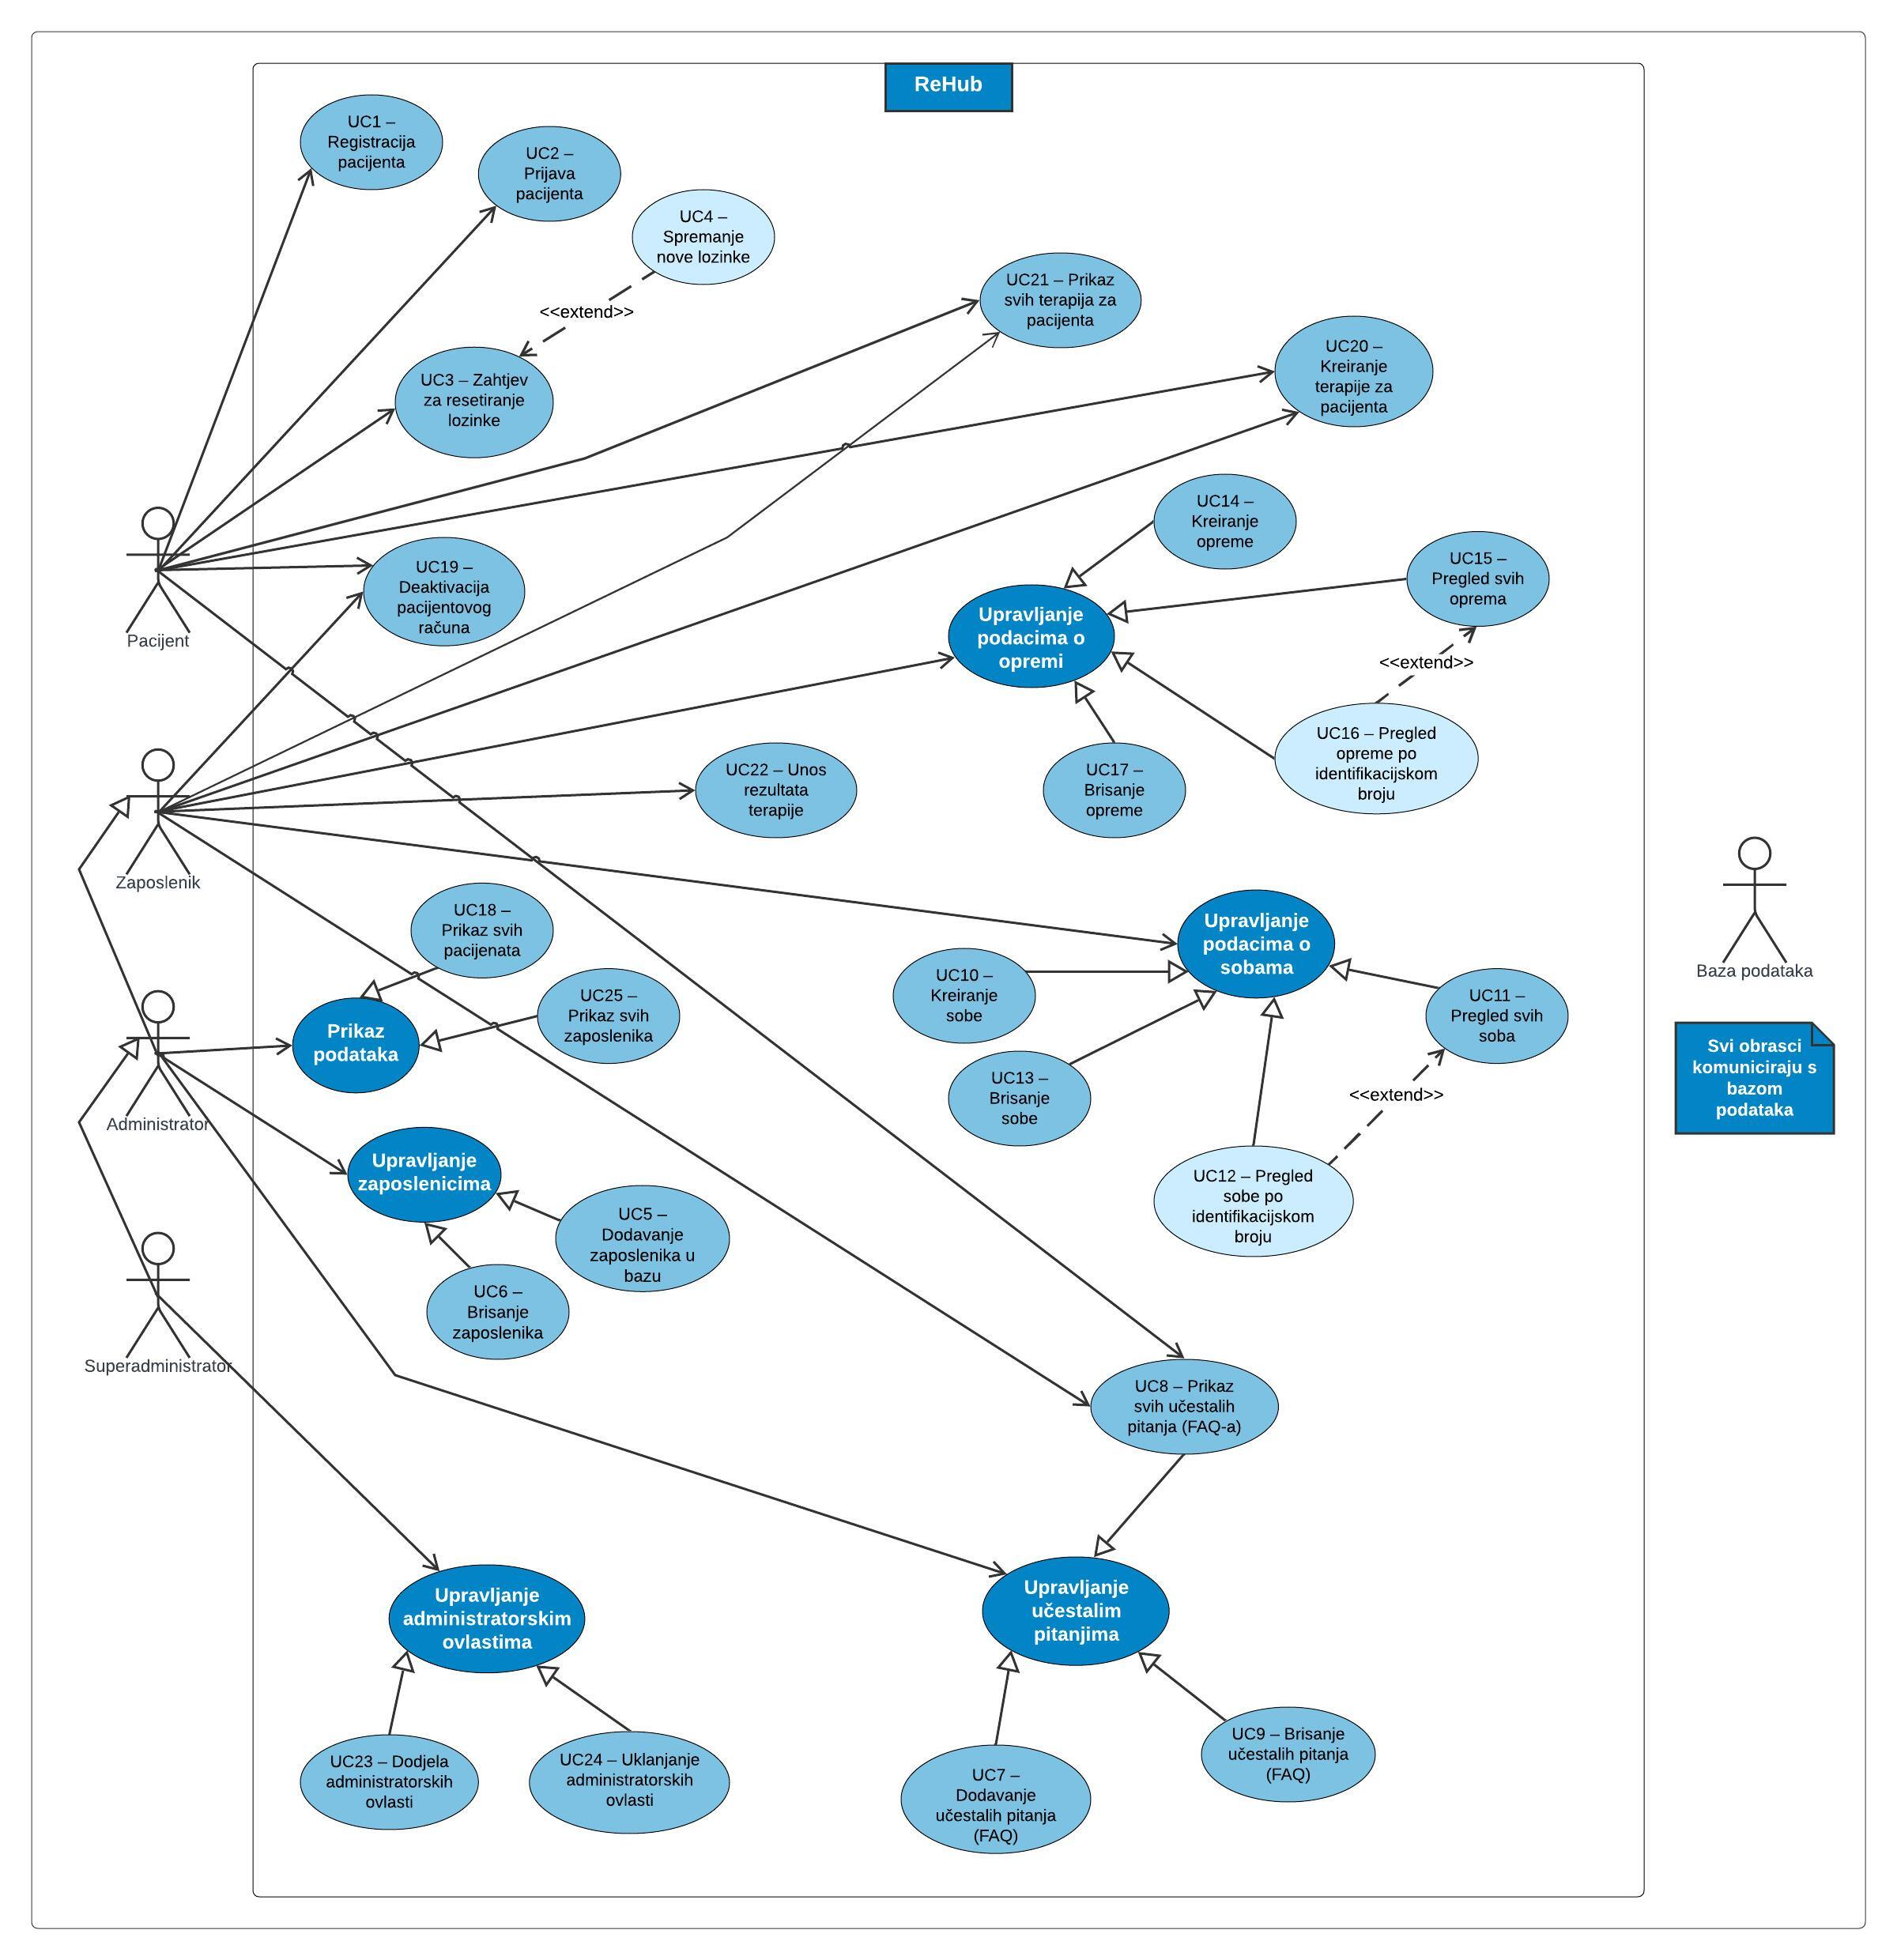
\includegraphics[scale=0.35]{dijagrami/ReHub Use case diagram.jpeg}
			         \centering
			         \caption{Dijagram obrazaca uporabe}
			         \label{fig:UseCaseDiagram}
		          \end{figure}
				\eject		
				
			\subsection{Sekvencijski dijagrami}
				
				U sljedećem dijelu prikazani su sekvencijski dijagrami i njihovi opisi.
                \subsubsection{Obrazac uporabe UC18 – Prikaz svih pacijenata i UC25 – Prikaz svih zaposlenika}

                    Korisnik odabire opciju "Prikaži sve pacijente" ili "Prikaži sve zaposlenike" unutar web-aplikacije. Web-aplikacija iz baze podataka dohvaća sve relevantne informacije o pacijentima odnosno zaposlenicima. Ako baza podataka vrati informacije o pacijentima, web-aplikacija ih prikazuje korisniku, omogućujući mu pregled detalja poput imena, adrese, kontakt informacija itd. U suprotnom, ispisuje poruku "Nema dostupnih pacijenata". Ako korisnik odabere opciju "Prikaži sve zaposlenike", web-aplikacija prikazuje informacije o svim zaposlenicima, uključujući njihova imena, pozicije, kontakt informacije itd. U suprotnom, ispisuje poruku "Nema dostupnih zaposlenika".

                \begin{figure}[H]
			         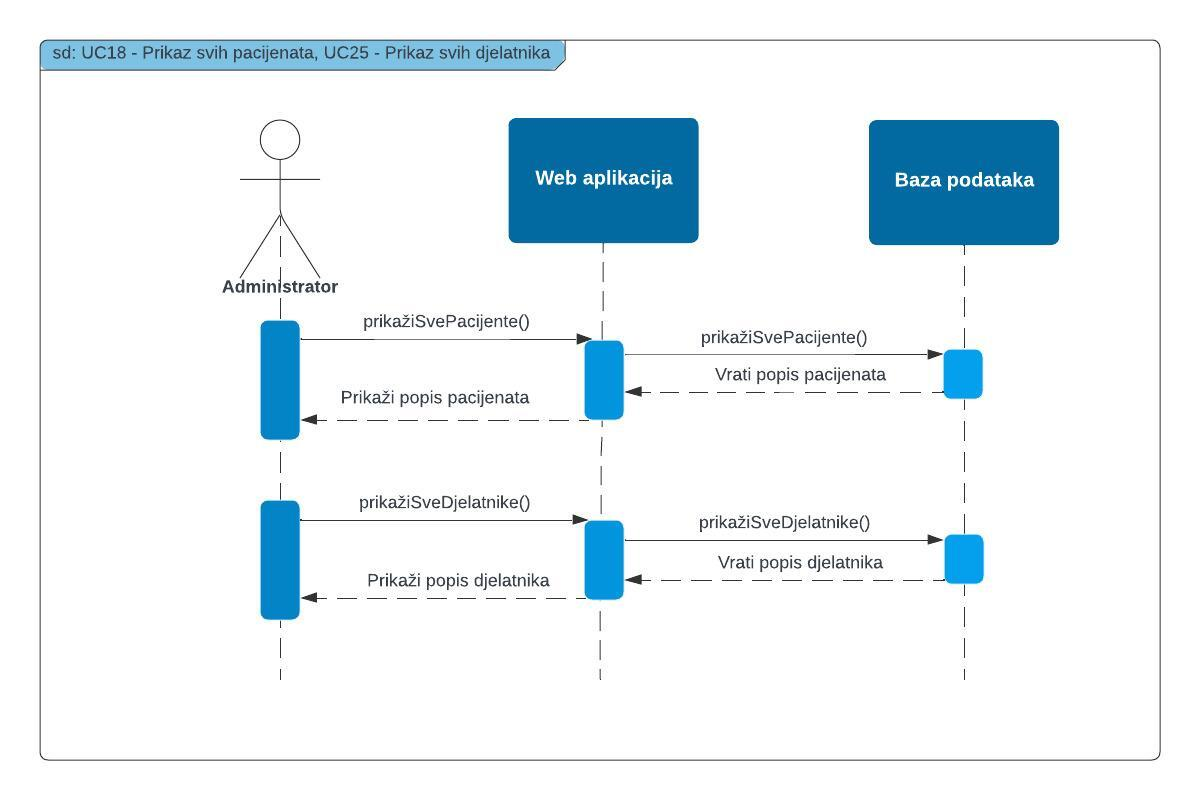
\includegraphics[scale=0.7]{dijagrami/Sequence diagram for ReHub admin.jpeg}
			         \centering
			         \caption{Sekvencijski dijagram za UC18/25}
			         \label{fig:SequenceDiagram1}
		        \end{figure}

                \eject

                \subsubsection{Obrazac uporabe UC8 – Prikaz svih učestalih pitanja, UC11 – Pregled svih soba i UC15 – Prikaz svih oprema}

                    Korisnik odabire opciju "Učestala pitanja" unutar web-aplikacije. Web-aplikacija iz baze podataka dohvaća sve učestala pitanja. Ako postoje učestala pitanja, aplikacija ih prikazuje korisniku, pružajući odgovore i relevantne informacije. Ako nema učestalih pitanja, ispisuje poruku "Nema dostupnih učestalih pitanja." Dodatna funkcionalnost: Korisnik ima mogućnost filtriranja pitanja po kategorijama ili ključnim riječima. Korisnik odabire opciju "Pregled svih soba" unutar web-aplikacije. Web-aplikacija iz baze podataka dohvaća sve informacije o sobama. Ako postoje sobe, aplikacija ih prikazuje korisniku s detaljima poput broja sobe, vrste, dostupnih sadržaja itd. Ako nema dostupnih soba, ispisuje poruku "Nema dostupnih soba." Dodatna funkcionalnost: Korisnik može filtrirati sobe prema vrsti, kapacitetu ili dostupnim sadržajima. Korisnik odabire opciju "Prikaz svih oprema" unutar web-aplikacije. Web-aplikacija iz baze podataka dohvaća informacije o svim dostupnim opremama. Ako postoje informacije o opremama, aplikacija ih prikazuje korisniku, pružajući detalje o vrstama opreme, količini dostupnih itd. Ako nema dostupnih informacija o opremama, ispisuje poruku "Nema dostupne opreme." Dodatna funkcionalnost: Korisnik može filtrirati opremu prema vrsti ili dostupnosti.

                    \begin{figure}[H]
			         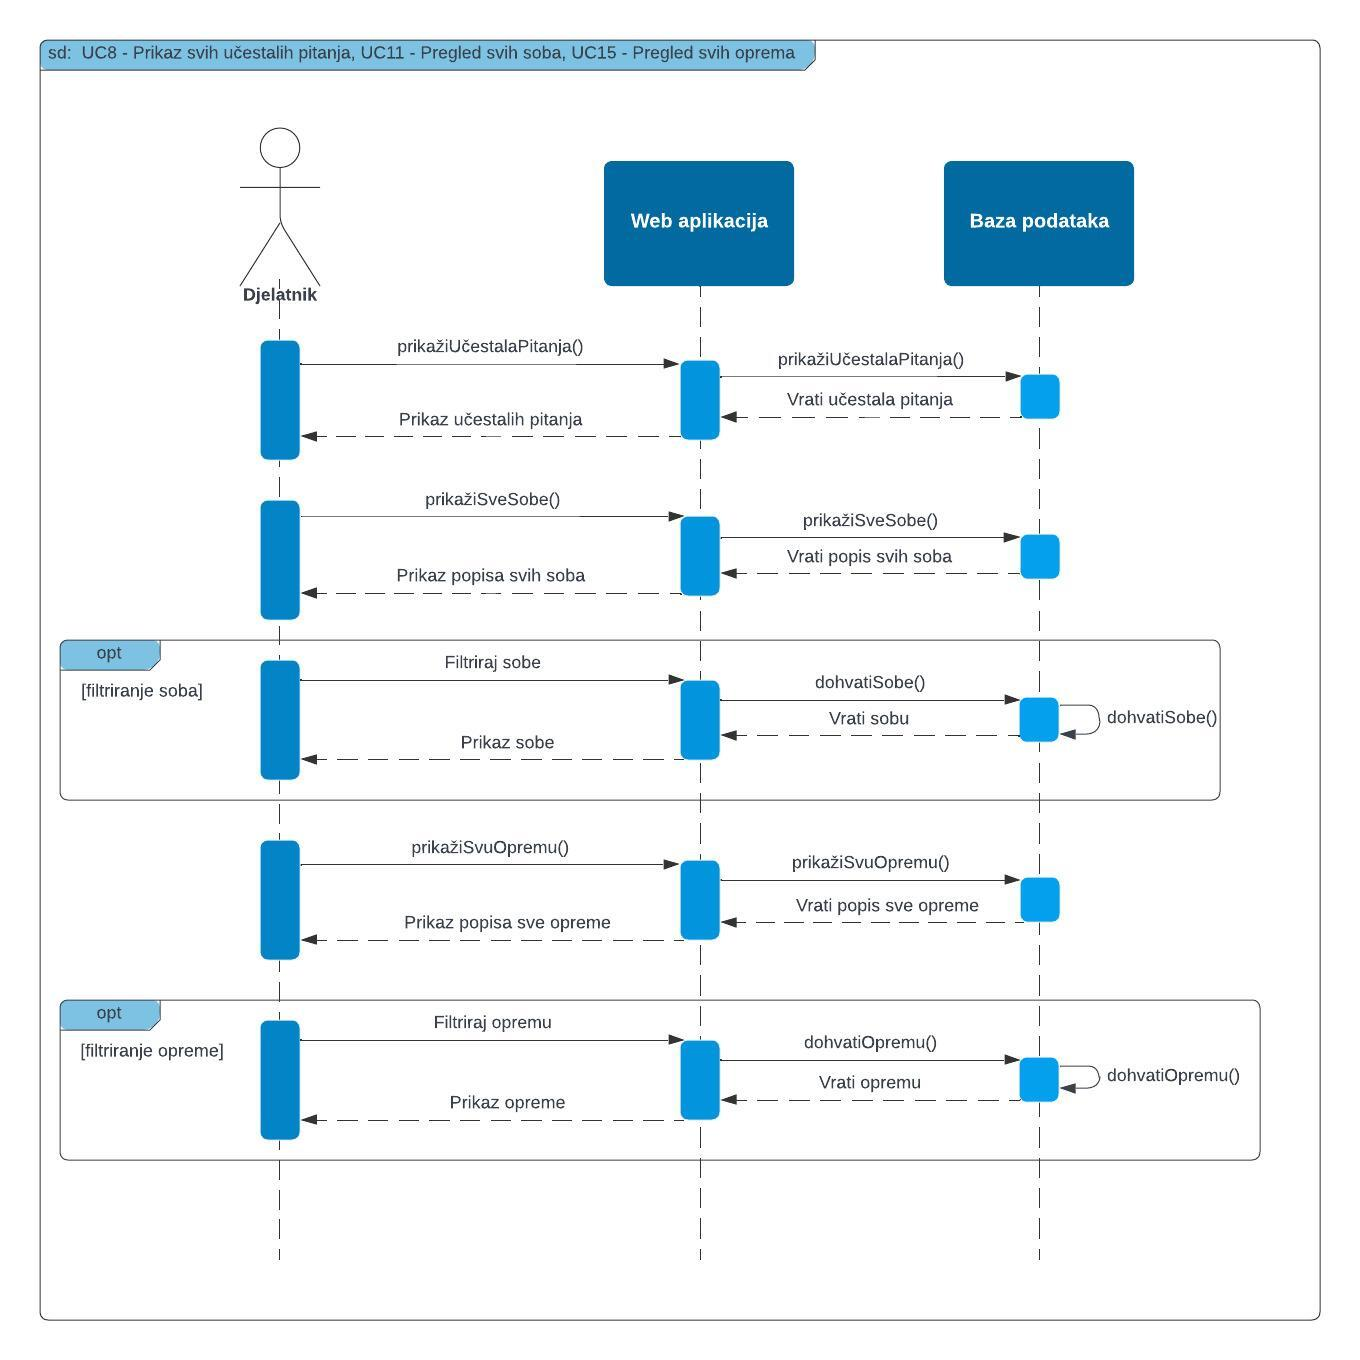
\includegraphics[scale=0.7]{dijagrami/Sequence diagram for ReHub.jpeg}
			         \centering
			         \caption{Sekvencijski dijagram za UC8/11/15}
			         \label{fig:SequenceDiagram2}
		          \end{figure}
                
				\eject
	
		\section{Ostali zahtjevi}
		 
			 \begin{packed_enum}
				
				\large \item Sustav mora podržavati više različitih uloga korisnika \normalsize
                    \begin{packed_item}
                        \item Sustav treba omogućiti definiranje različitih razina pristupa i funkcionalnosti ovisno o ulozi korisnika (Administrator, Liječnik, Pacijent, itd.).
                    \end{packed_item}
				 \large \item Korisnički podaci moraju biti sigurno pohranjeni u sustavu	\normalsize
                    \begin{packed_item}
                        \item Sustav treba koristiti kriptiranje za pohranu i prijenos osjetljivih korisničkih podataka kako bi osigurao privatnost i sigurnost informacija.
                    \end{packed_item}
				 \large \item Brza i pouzdana veza s bazom podataka \normalsize
                    \begin{packed_item}
                        \item Sustav treba osigurati pouzdanu vezu s bazom podataka kako bi pristup podacima bio brz i otporan na vanjske pogreške.
                    \end{packed_item}
                 \large \item Odgovarajuće vrijeme izvršavanja za upite prema bazi podataka \normalsize
                    \begin{packed_item}
                        \item Izvršavanje upita koji pristupaju bazi podataka ne smije trajati dulje od definiranog vremena, kako bi se osigurala učinkovitost sustava.
                    \end{packed_item}
                 \large \item Podrška za hrvatsku abecedu u korisničkom sučelju i pri unosu teksta \normalsize
                    \begin{packed_item}
                        \item Korisničko sučelje i sustav trebaju podržavati hrvatsku abecedu pri unosu, prikazu i obradi tekstualnih podataka.
                    \end{packed_item}
                 \large \item Web aplikacija implementirana korištenjem objektno-orijentiranih jezika \normalsize
                    \begin{packed_item}
                        \item Sustav treba biti implementiran kao web aplikacija koristeći suvremene objektno-orijentirane jezike kako bi bio skalabilan i održiv.
                    \end{packed_item}
                 \large \item Intuitivan i lagan za korištenje \normalsize
                    \begin{packed_item}
                        \item Korisničko sučelje treba biti intuitivno i jednostavno za korištenje kako bi korisnici mogli efikasno koristiti sustav bez potrebe za dodatnim uputama.
                    \end{packed_item}
                 \large \item Nadogradnja sustava bez narušavanja postojećih funkcionalnosti \normalsize
                    \begin{packed_item}
                        \item Nadogradnje sustava trebaju biti provedene bez negativnog utjecaja na postojeće funkcionalnosti kako bi korisnici nastavili neometano koristiti sustav.
                    \end{packed_item}
                 \large \item Zaštita od neispravnog korištenja korisničkog sučelja \normalsize
                    \begin{packed_item}
                        \item Neispravno korištenje korisničkog sučelja ne smije narušiti funkcionalnosti i rad sustava. Sustav treba biti otporan na potencijalne greške ili zloupotrebu od strane korisnika.
                    \end{packed_item}
                    
				
			\end{packed_enum}
			 
			 
			 
	
	\chapter{Arhitektura i dizajn sustava}

Rehub predstavlja sofisticirano arhitektonsko rješenje koje integrira PostgreSQL bazu podataka, Spring Boot za backend logiku, React za korisničko sučelje, te Tailwind CSS za moderno i responzivno oblikovanje. Sustav je implementiran na cloud platformama Render za backend i bazu te Netlify za frontend, koristeći njihove usluge za brz, skalabilan i pouzdan deploying.\\

\begin{packed_item}
	\large \item Baza podataka: PostgreSQL \normalsize \\
	PostgreSQL, snažan sustav za upravljanje relacijskim bazama podataka, predstavlja ključnu komponentu u arhitekturi ove web aplikacije. Struktura baze podataka temeljito je dizajnirana kako bi zadovoljila specifične zahtjeve aplikacije. Kroz pažljivu integraciju s PostgreSQL-om, aplikacija ostvaruje brz i učinkovit pristup podacima, čime se osigurava optimalna performansa. Ova konfiguracija baze podataka predstavlja ključnu komponentu cjelokupnog arhitektonskog rješenja, pružajući čvrstu temeljnu strukturu za rad backend sustava. \\
	\large \item Backend: Spring Boot \normalsize \\
	Spring Boot, kao Java-based framework, pruža snažan temelj za razvoj backend logike. Ova web aplikacija koristi Spring Boot za stvaranje RESTful API-ja koji komunicira s PostgreSQL bazom podataka. Ovo rješenje omogućuje efikasno upravljanje podacima i pruža mogućnost proširivosti sustava kroz modularnost i lakoću integracije. \\
	\large \item Frontend: React \normalsize \\
	React, centralna JavaScript biblioteka, određuje arhitekturu frontend dijela ove aplikacije. Modularne React komponente omogućuju čist i jednostavan kod, prilagodljiv specifičnim zahtjevima sučelja. Ovaj pristup omogućuje stvaranje brzog, dinamičkog korisničkog sučelja koje se lako održava. Kroz React, osigurava se fluidna navigacija kroz aplikaciju, pridonoseći ukupnom intuitivnom korisničkom iskustvu. \\
	\large \item Frontend Integracija: Tailwind CSS, Axios, React-Router-Dom, reCAPTCHA \normalsize \\
	Frontend aplikacije unaprijeđen je integracijom Tailwind CSS za brzo oblikovanje sučelja, Axios za efikasnu komunikaciju s backendom, React-Router-Dom za fluidnu navigaciju te reCAPTCHA sustava radi dodatne sigurnosti. Tailwind CSS pridonosi estetskom izgledu, Axios omogućuje dinamičku interakciju s backendom, React-Router-Dom olakšava upravljanje rutama, dok reCAPTCHA sprječava zlonamjerne aktivnosti. Kroz ovu integraciju postiže se uravnoteženo frontend rješenje koje kombinira funkcionalnost, estetiku i sigurnost korisničkog iskustva. \\
	\large \item Deployment: Render za backend i Netlify za frontend \normalsize \\
	Backend i baza podataka su postavljeni na Render platformu za optimalno upravljanje resursima. Render osigurava automatsko skaliranje i brzu dostupnost aplikacije koristeći njihove cloud usluge. Na renderu je također podešeno kontinuirano postavljanje koje omogućuje automatsko ažuriranje softvera. Frontend je zasebno postavljen na Netlify platformi, koja pruža brzo i globalno dostupno CDN (Content Delivery Network). \\
\end{packed_item}

Rehub predstavlja integrirano arhitektonsko rješenje koje kombinira najbolje prakse u razvoju aplikacija, pružajući stabilnost, skalabilnost i visoku razinu korisničkog iskustva. Korištenje navedenih tehnologija i servisa osigurava da aplikacija bude spremna za izazove suvremenog web razvoja.




\begin{figure}[H]
	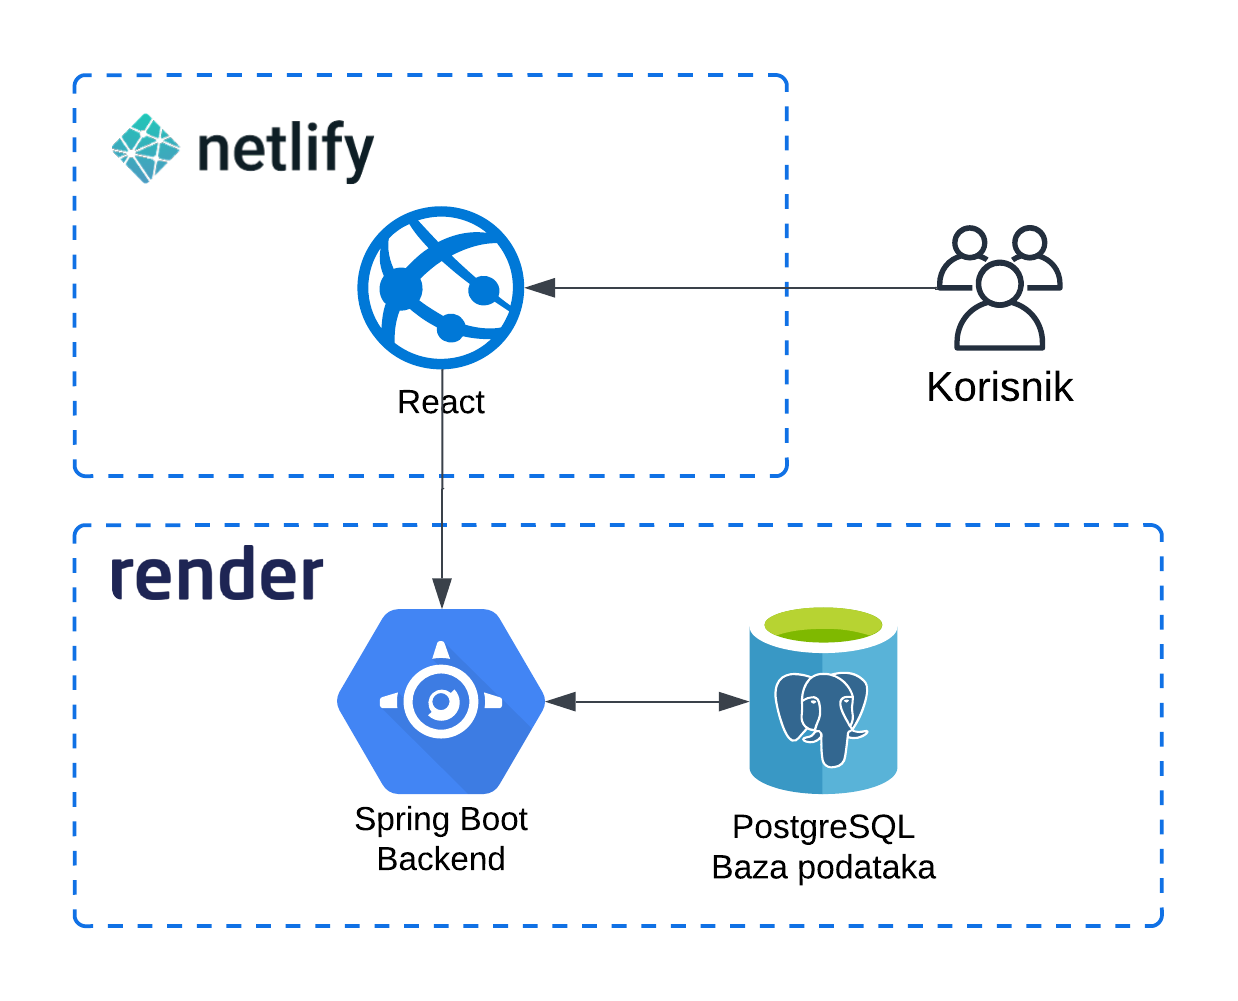
\includegraphics[scale=0.25]{dijagrami/architecture_diagram.png}
	\centering
	\caption{Dijagram arhitekture}
	\label{fig:architecture_diagram}
\end{figure}

\section{Baza podataka}

U bazi su stvorene relacije koje olakšavaju jednostavno rukovanje podacima, uključujući dodavanje, brisanje, izmjenu i dohvaćanje podataka. Svi entiteti i relacije su organizirani prema trećoj normalnoj formi kako bi se izbjegla redundancija podataka. Za bolje vizualiziranje strukture baze podataka, napravljen je relacijski dijagram koji je prikazan u nastavku. \\
\\
Baza podataka se sastoji od tablica (relacija) koje su definirane svojim imenom i skupom
atributa. Baza podataka ove aplikacije sastoji se od sljedećih entiteta:

\begin{packed_item}
	\item rehub\_user
	\item employee
	\item user\_role
	\item role
	\item patient
	\item therapy
	\item therapy\_result
	\item doctor
	\item appointment
	\item room
	\item equipment
	\item faq
	\item personal\_data
	\item verification
	\item password\_reset
	\item flyway\_history\_schema
\end{packed_item}


\subsection{Opis tablica}

Prva ćelija svake tablice označava njeno ime. U prvom stupcu navedeni su atributi tog entiteta, u drugom stupcu naveden je tip varijable, a u trećem opis svakog pojedinog atributa. Svjetlozelenom bojom označeni su primarni ključevi. Svjetlo plavom označeni su strani ključevi. \\	


\begin{longtblr}[
	label=none,
	entry=none,
	]{
		width=\textwidth,
		colspec={|X[6,l]|X[6,l]|X[20,l]|}, 
		rowhead=1,
	}
	\hline
	\SetCell[c=3]{c}{\textbf{rehub\_user}} \\ \hline[3pt]
	\SetCell{LightGreen} ID & BIGSERIAL & JEDINSTVENI IDENTIFIKATOR KORISNIKA \\ \hline
	USERNAME & VARCHAR & KORISNIČKO IME S KOJIM SE KORISNIK PRIJAVLJUJE \\ \hline
	PASSWORD & VARCHAR & LOZINKA S KOJOM SE KORISNIK PRIJAVLJUJE \\ \hline
	STATUS & VARCHAR & STATUS KORISNIKA \\ \hline
	\SetCell{LightBlue} PERSONAL\_DATA\_ID & VARCHAR & JEDINSTVENI IDENTIFIKATOR KORISNIKA \\ \hline
\end{longtblr}

Entitet označava korisnika aplikacije te sadrži atribute: id, username, password, status, personal\_data\_id.

% Table 2: employee
\begin{longtblr}[
	label=none,
	entry=none,
	]{
		width=\textwidth,
		colspec={|X[6,l]|X[6,l]|X[20,l]|}, 
		rowhead=1,
	}
	\hline
	\SetCell[c=3]{c}{\textbf{employee}} \\ \hline[3pt]
	\SetCell{LightGreen} ID & BIGSERIAL & JEDINSTVENI IDENTIFIKATOR ZAPOSLENIKA \\ \hline
	FIRST\_NAME & VARCHAR & IME ZAPOSLENIKA \\ \hline
	LAST\_NAME & VARCHAR & PREZIME ZAPOSLENIKA \\ \hline
	PHONE\_NUMBER & VARCHAR & BROJ MOBITELA ZAPOSLENIKA \\ \hline
	PROFESSION & VARCHAR & STRUKA ZAPOSLENIKA \\ \hline
	GENDER & VARCHAR & SPOL ZAPOSLENIKA \\ \hline
	CREATED\_AT & TIMESTAMP & TRENUTAK KREIRANJA \\ \hline
	LAST\_MODIFIED\_AT & TIMESTAMP & TRENUTAK ZADNJE PROMJENE \\ \hline
	\SetCell{LightBlue} USER\_ID & VARCHAR & JEDINSTVENI IDENTIFIKATOR KORISNIKA \\ \hline
\end{longtblr}

Entitet označava osobe zaposlene u klinici. Atributi ovoga entiteta su: id, first\_name, last\_name, phone\_number, profession, gender, created\_at, last\_modified\_at, user\_id.

% Table 3: user_role
\begin{longtblr}[
	label=none,
	entry=none,
	]{
		width=\textwidth,
		colspec={|X[6,l]|X[6,l]|X[20,l]|}, 
		rowhead=1,
	}
	\hline
	\SetCell[c=3]{c}{\textbf{user\_role}} \\ \hline[3pt]
	\SetCell{LightBlue} USER\_ID & BIGSERIAL & JEDINSTVENI IDENTIFIKATOR KORISNIKA \\ \hline
	\SetCell{LightBlue} ROLE\_ID & BIGSERIAL & JEDINSTVENI IDENTIFIKATOR VRSTE KORISNIKA \\ \hline
\end{longtblr}

Entitet označava vrstu korisnika aplikacije, a njegovi atributi su: user\_id, role\_id.

% Table 4: role
\begin{longtblr}[
	label=none,
	entry=none,
	]{
		width=\textwidth,
		colspec={|X[6,l]|X[6,l]|X[20,l]|}, 
		rowhead=1,
	}
	\hline
	\SetCell[c=3]{c}{\textbf{role}} \\ \hline[3pt]
	\SetCell{LightGreen} ID & BIGSERIAL & JEDINSTVENI IDENTIFIKATOR ULOGE \\ \hline
	NAME & VARCHAR & IME ULOGE \\ \hline
\end{longtblr}

Entitet označava ulogu i sastoji se od atributa: id, name.

% Table 5: patient
\begin{longtblr}[
	label=none,
	entry=none,
	]{
		width=\textwidth,
		colspec={|X[6,l]|X[6,l]|X[20,l]|}, 
		rowhead=1,
	}
	\hline
	\SetCell[c=3]{c}{\textbf{patient}} \\ \hline[3pt]
	\SetCell{LightGreen} ID & BIGSERIAL & JEDINSTVENI IDENTIFIKATOR PACIJENTA \\ \hline
	FIRST\_NAME & VARCHAR & IME PACIJENTA \\ \hline
	LAST\_NAME & VARCHAR & PREZIME PACIJENTA \\ \hline
	GENDER & VARCHAR & SPOL PACIJENTA \\ \hline
	PHONE\_NUMBER & VARCHAR & BROJ MOBITELA PACIJENTA \\ \hline
	DATE\_OF\_BIRTH & DATE & DATUM ROĐENJA PACIJENTA \\ \hline
	CREATED\_AT & TIMESTAMP & TRENUTAK KREIRANJA \\ \hline
	LAST\_MODIFIED\_AT & TIMESTAMP & TRENUTAK ZADNJE PROMJENE \\ \hline
	\SetCell{LightBlue} USER\_ID & BIGSERIAL & JEDINSTVENI IDENTIFIKATOR KORISNIKA \\ \hline
\end{longtblr}

Entitet predstavlja pacijenta koji je korisnik aplikacije. Atributi su: id, first\_name, last\_name, gender, phone\_number, date\_of\_birth, created\_at, last\_modified\_at, user\_id.

% Table 6: therapy
\begin{longtblr}[
	label=none,
	entry=none,
	]{
		width=\textwidth,
		colspec={|X[6,l]|X[6,l]|X[20,l]|}, 
		rowhead=1,
	}
	\hline
	\SetCell[c=3]{c}{\textbf{therapy}} \\ \hline[3pt]
	\SetCell{LightGreen} ID & BIGSERIAL & JEDINSTVENI IDENTIFIKATOR TERAPIJE \\ \hline
	TYPE & VARCHAR & VRSTA TERAPIJE \\ \hline
	REQUEST & VARCHAR & ZAHTJEV ZA TERAPIJOM \\ \hline
	STATUS & VARCHAR & STATUS TERAPIJE \\ \hline
	REF\_ID & BIGSERIAL & JEDINSTVENI IDENTIFIKATOR \\ \hline
	CREATED\_AT & TIMESTAMP & TRENUTAK KREIRANJA \\ \hline
	LAST\_MODIFIED\_AT & TIMESTAMP & TRENUTAK ZADNJE PROMJENE \\ \hline
	\SetCell{LightBlue} PATIENT\_ID & BIGSERIAL & JEDINSTVENI IDENTIFIKATOR PACIJENTA \\ \hline
	\SetCell{LightBlue} EMPLOYEE\_ID & BIGSERIAL & JEDINSTVENI IDENTIFIKATOR ZAPOSLENIKA \\ \hline
	\SetCell{LightBlue} ROOM\_ID & BIGSERIAL & JEDINSTVENI IDENTIFIKATOR SOBE \\ \hline
	\SetCell{LightBlue} APPOINTMENT\_ID & BIGSERIAL & JEDINSTVENI IDENTIFIKATOR TERMINA \\ \hline
	\SetCell{LightBlue} THERAPY\_RESULT\_ID & BIGSERIAL & JEDINSTVENI IDENTIFIKATOR REZULTATA TERAPIJE \\ \hline
	DOCTOR\_FULL\_NAME & VARCHAR & PUNO IME DOKTORA \\ \hline
	THERAPY\_SCAN & VARCHAR & NAZIV UPUTNICE ZA TERAPIJU \\ \hline
\end{longtblr}

Entitet opisuje terapiju dodijeljenu pacijentu. Njeni atributi su: id, type, request, status, ref\_id, created\_at, last\_modified\_at, patient\_id, employee\_id, room\_id, appointment\_id, therapy\_result\_id, doctor\_full\_name, therapy\_scan.

% Table 7: doctor
\begin{longtblr}[
	label=none,
	entry=none,
	]{
		width=\textwidth,
		colspec={|X[6,l]|X[6,l]|X[20,l]|}, 
		rowhead=1,
	}
	\hline
	\SetCell[c=3]{c}{\textbf{doctor}} \\ \hline[3pt]
	\SetCell{LightGreen}ID & BIGSERIAL & JEDINSTVENI IDENTIFIKATOR DOKTORA \\ \hline
	FIRST\_NAME & VARCHAR & IME DOKTORA \\ \hline
	LAST\_NAME & VARCHAR & PREZIME DOKTORA \\ \hline
	PIN & VARCHAR & PIN DOKTORA \\ \hline
	MEDICAL\_NO & VARCHAR & MEDICINSKI BROJ \\ \hline
	SPECIALITY & VARCHAR & DOKTOROVA SPECIJALIZACIJA \\ \hline
	DATE\_OF\_EMPLOYMENT & DATE & DATUM ZAPOSLENJA \\ \hline
	DATE\_OF\_REGISTRATION & DATE & DATUM REGISTRACIJE \\ \hline
	DATE\_OF\_BIRTH & TIMESTAMP & DATUM ROĐENJA \\ \hline
\end{longtblr}

Entitet predstavlja doktora koji je korisnik aplikacije. Atributi su: id, first\_name, last\_name, pin, medical\_no, speciality, date\_of\_employment, date\_of\_registration, date\_of\_birth.

% Table 8: appointment
\begin{longtblr}[
	label=none,
	entry=none,
	]{
		width=\textwidth,
		colspec={|X[6,l]|X[6,l]|X[20,l]|}, 
		rowhead=1,
	}
	\hline
	\SetCell[c=3]{c}{\textbf{appointment}} \\ \hline[3pt]
	\SetCell{LightGreen}ID & BIGSERIAL & JEDINSTVENI IDENTIFIKATOR TERMINA \\ \hline
	START\_AT & TIMESTAMP & POČETAK TERMINA \\ \hline
	END\_AT & TIMESTAMP & KRAJ TERMINA \\ \hline
\end{longtblr}

Entitet predstavlja termin na koji se pacijent naručio, a atributi su: id, start\_at, end\_at.

% Table 9: therapy_result
\begin{longtblr}[
	label=none,
	entry=none,
	]{
		width=\textwidth,
		colspec={|X[6,l]|X[6,l]|X[20,l]|}, 
		rowhead=1,
	}
	\hline
	\SetCell[c=3]{c}{\textbf{therapy\_result}} \\ \hline[3pt]
	\SetCell{LightGreen}ID & BIGSERIAL & JEDINSTVENI IDENTIFIKATOR REZULTATA TERAPIJE \\ \hline
	STATUS & VARCHAR & STATUS TERAPIJE \\ \hline
	RESULT & VARCHAR & KONAČNI REZULTAT TERAPIJE \\ \hline
\end{longtblr}

Ovaj entitet predstavlja rezultat terapije, a definiran je sljedećim atributima: id, status, result.

% Table 10: room
\begin{longtblr}[
	label=none,
	entry=none,
	]{
		width=\textwidth,
		colspec={|X[6,l]|X[6,l]|X[20,l]|}, 
		rowhead=1,
	}
	\hline
	\SetCell[c=3]{c}{\textbf{room}} \\ \hline[3pt]
	\SetCell{LightGreen}ID & BIGSERIAL & JEDINSTVENI IDENTIFIKATOR SOBE \\ \hline
	LABEL & VARCHAR & OZNAKA SOBE \\ \hline
	CAPACITY & BIGSERIAL & KAPACITET SOBE \\ \hline
	STATUS & VARCHAR & STATUS O KORIŠTENJU SOBE \\ \hline
	SPECIAL\_MESSAGE & VARCHAR & NAPOMENA \\ \hline
\end{longtblr}

Entitet predstavlja sobu u kojoj se odvija terapija, a njeni atributi su: id, label, capacity, status, special\_message.

% Table 11: equipment
\begin{longtblr}[
	label=none,
	entry=none,
	]{
		width=\textwidth,
		colspec={|X[6,l]|X[6,l]|X[20,l]|}, 
		rowhead=1,
	}
	\hline
	\SetCell[c=3]{c}{\textbf{equipment}} \\ \hline[3pt]
	\SetCell{LightGreen}ID & BIGSERIAL & JEDINSTVENI IDENTIFIKATOR OPREME \\ \hline
	NAME & VARCHAR & IME OPREME \\ \hline
	STATUS & VARCHAR & STATUS O KORIŠTENJU OPREME \\ \hline
	SPECIAL\_MESSAGE & VARCHAR & NAPOMENA \\ \hline
	\SetCell{LightBlue}ROOM\_ID & BIGSERIAL & JEDINSTVENI IDENTIFIKATOR SOBE \\ \hline
\end{longtblr}

Ovaj entiet se odnosi na opremu koja se koristi prilikom terapije, a opisuju ju: id, name, status, special\_message, room\_id.

% Table 12: personal_data
\begin{longtblr}[
	label=none,
	entry=none,
	]{
		width=\textwidth,
		colspec={|X[6,l]|X[6,l]|X[20,l]|}, 
		rowhead=1,
	}
	\hline
	\SetCell[c=3]{c}{\textbf{personal\_data}} \\ \hline[3pt]
	\SetCell{LightGreen}ID & BIGSERIAL & JEDINSTVENI IDENTIFIKATOR KORISNIKA \\ \hline
	FIRST\_NAME & VARCHAR & IME KORISNIKA \\ \hline
	LAST\_NAME & VARCHAR & PREZIME KORISNIKA \\ \hline
	PIN & VARCHAR & OIB KORISNIKA \\ \hline
	PHIN & VARCHAR & MATIČNI BROJ KORISNIKA \\ \hline
	DATE\_OF\_BIRTH & DATE & DATUM ROĐENJA KORISNIKA \\ \hline
\end{longtblr}

Ovaj entitet sadrži osobne podatke o korisniku aplikacije, a atributi su mu: id, first\_name, last\_name, pin, phin i date\_of\_birth.

% Table 13: faq
\begin{longtblr}[
	label=none,
	entry=none,
	]{
		width=\textwidth,
		colspec={|X[6,l]|X[6,l]|X[20,l]|}, 
		rowhead=1,
	}
	\hline
	\SetCell[c=3]{c}{\textbf{faq}} \\ \hline[3pt]
	\SetCell{LightGreen}ID & BIGSERIAL & JEDINSTVENI IDENTIFIKATOR PITANJA I ODGOVORA \\ \hline
	QUESTION & VARCHAR & PITANJE \\ \hline
	ANSWER & VARCHAR & ODGOVOR \\ \hline
\end{longtblr}

Entitet se odnosi na često postavljena pitanja i sastoji se od sljedećih atributa: id, question te answer.

% Table 14: verification
\begin{longtblr}[
	label=none,
	entry=none,
	]{
		width=\textwidth,
		colspec={|X[6,l]|X[6,l]|X[20,l]|}, 
		rowhead=1,
	}
	\hline
	\SetCell[c=3]{c}{\textbf{verification}} \\ \hline[3pt]
	\SetCell{LightGreen}ID & BIGSERIAL & JEDINSTVENI IDENTIFIKATOR VERIFIKACIJE \\ \hline
	TOKEN & VARCHAR & TOKEN VERIFIKACIJE \\ \hline
	STATUS & VARCHAR & STATUS VERIFIKACIJE \\ \hline
	\SetCell{LightBlue}USER\_ID & BIGSERIAL & JEDINSTVENI IDENTIFIKATOR KORISNIKA \\ \hline
\end{longtblr}

Entitet se odnosi na verifikaciju i sastoji se od sljedećih atributa: id, token, status i user\_id.

% Table 15: password_reset
\begin{longtblr}[
	label=none,
	entry=none,
	]{
		width=\textwidth,
		colspec={|X[6,l]|X[6,l]|X[20,l]|}, 
		rowhead=1,
	}
	\hline
	\SetCell[c=3]{c}{\textbf{password\_reset}} \\ \hline[3pt]
	\SetCell{LightGreen}ID & BIGSERIAL & JEDINSTVENI IDENTIFIKATOR PONOVNOG POSTAVLJANJA LOZINKE \\ \hline
	TOKEN & VARCHAR & TOKEN PONOVNOG POSTAVLJANJA LOZINKE \\ \hline
	STATUS & VARCHAR & STATUS PONOVNOG POSTAVLJANJA LOZINKE \\ \hline
	\SetCell{LightBlue}USER\_ID & BIGSERIAL & JEDINSTVENI IDENTIFIKATOR KORISNIKA \\ \hline
	CREATED\_AT & TIMESTAMP & TRENUTAK KREIRANJA \\ \hline
	LAST\_MODIFIED\_AT & TIMESTAMP & ZADNJE MIJENJANO \\ \hline
\end{longtblr}

Entitet se odnosi na ponovno postavljanje lozinke i sastoji se od sljedećih atributa: id, token, status, user\_id, created\_at i last\_modified\_at.





\subsection{Dijagram baze podataka}

\begin{figure}[H]
	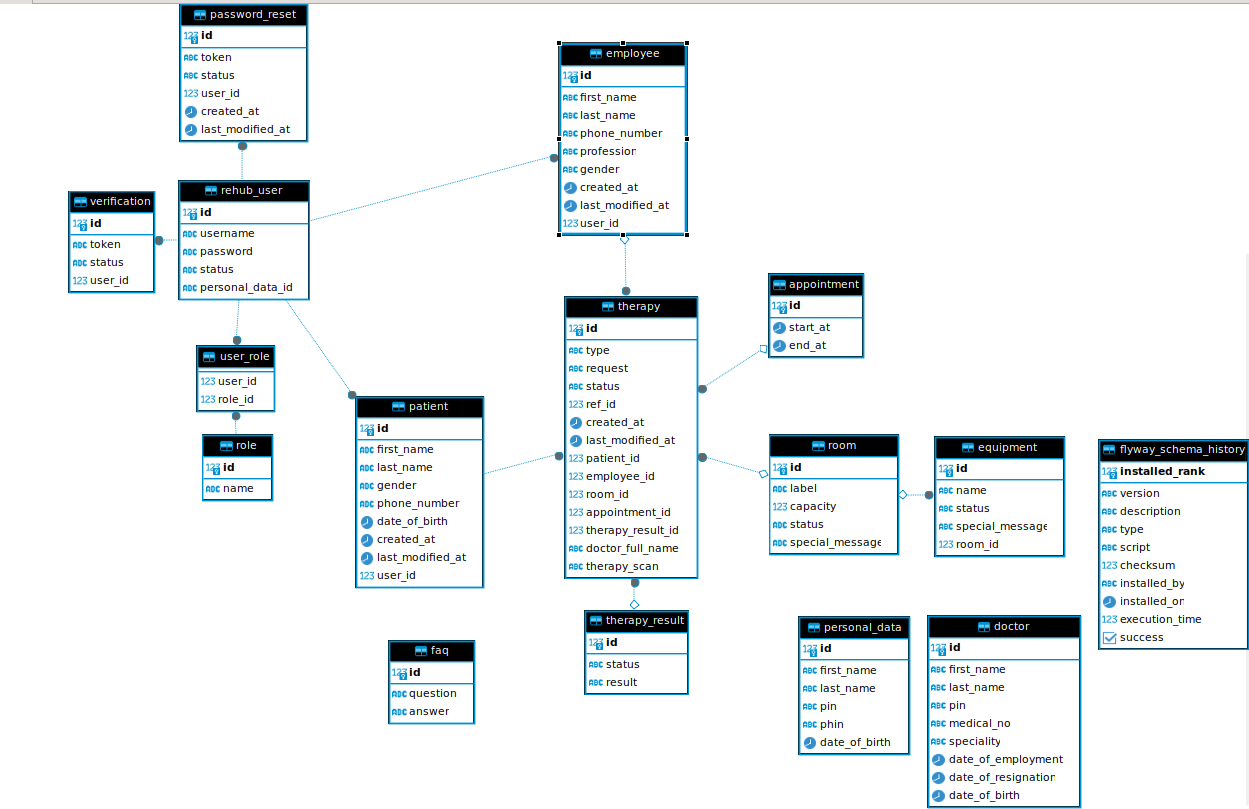
\includegraphics[scale=0.35]{dijagrami/rehub_db_diagram.png}
	\centering
	\caption{Dijagram baze podataka}
	\label{fig:dbDiagram}
\end{figure}

\eject


\section{Dijagram razreda}

Dijagramom razreda prikazujemo razrede u sustavu, njihove atribute i metode te veze između razreda koji se nasljeđuju ili međusobno komuniciraju. U nastavku slijede dijagrami čiji razredi imaju sličnu funkcionalnost i razinu apstrakcije

EntityClassDiagram - prikazuje razrede koji pripadaju sloju Model. Svaki od razreda se preslikava u odgovarajuću tablicu u bazi

RepositoryClassDiagram – prikazuje razrede koji pripadaju sloju Repository. Ovaj sloj komunicira sa bazom podataka i sa slojem Service.

ServiceClassDiagram – prikazuje razrede koji pripadaju sloju Service. Ovaj sloj komunicira sa slojem Repository i Controller.

ControllerClassDiagram – prikazuje razrede sloja Controller. Ovaj sloj komunicira sa slojem Service i s frontend dijelom aplikacije.

EnumClassDiagram – prikazuje enumeracije koje koristi sloj Model.

ConfigClassDiagram – prikazuje razrede sloja Config. Ovaj sloj služi za sigurnosne potrebe i komuniciranje putem e-maila.

SecurityClassDiagram - prikazuje razrede sloja Security. Ovaj sloj služi za sigurnost i detalje o korisniku.

RequestClassDiagram – prikazuje razrede sloja Request. Ovaj sloj komunicira sa slojem Controller u svrhu validacije Post Request-a.

ResponseClassDiagram – prikazuje razrede sloja Response. Ovaj sloj komunicira sa slojem Controller u svrhu vraćanja Response poruke.

\begin{figure}[H]
	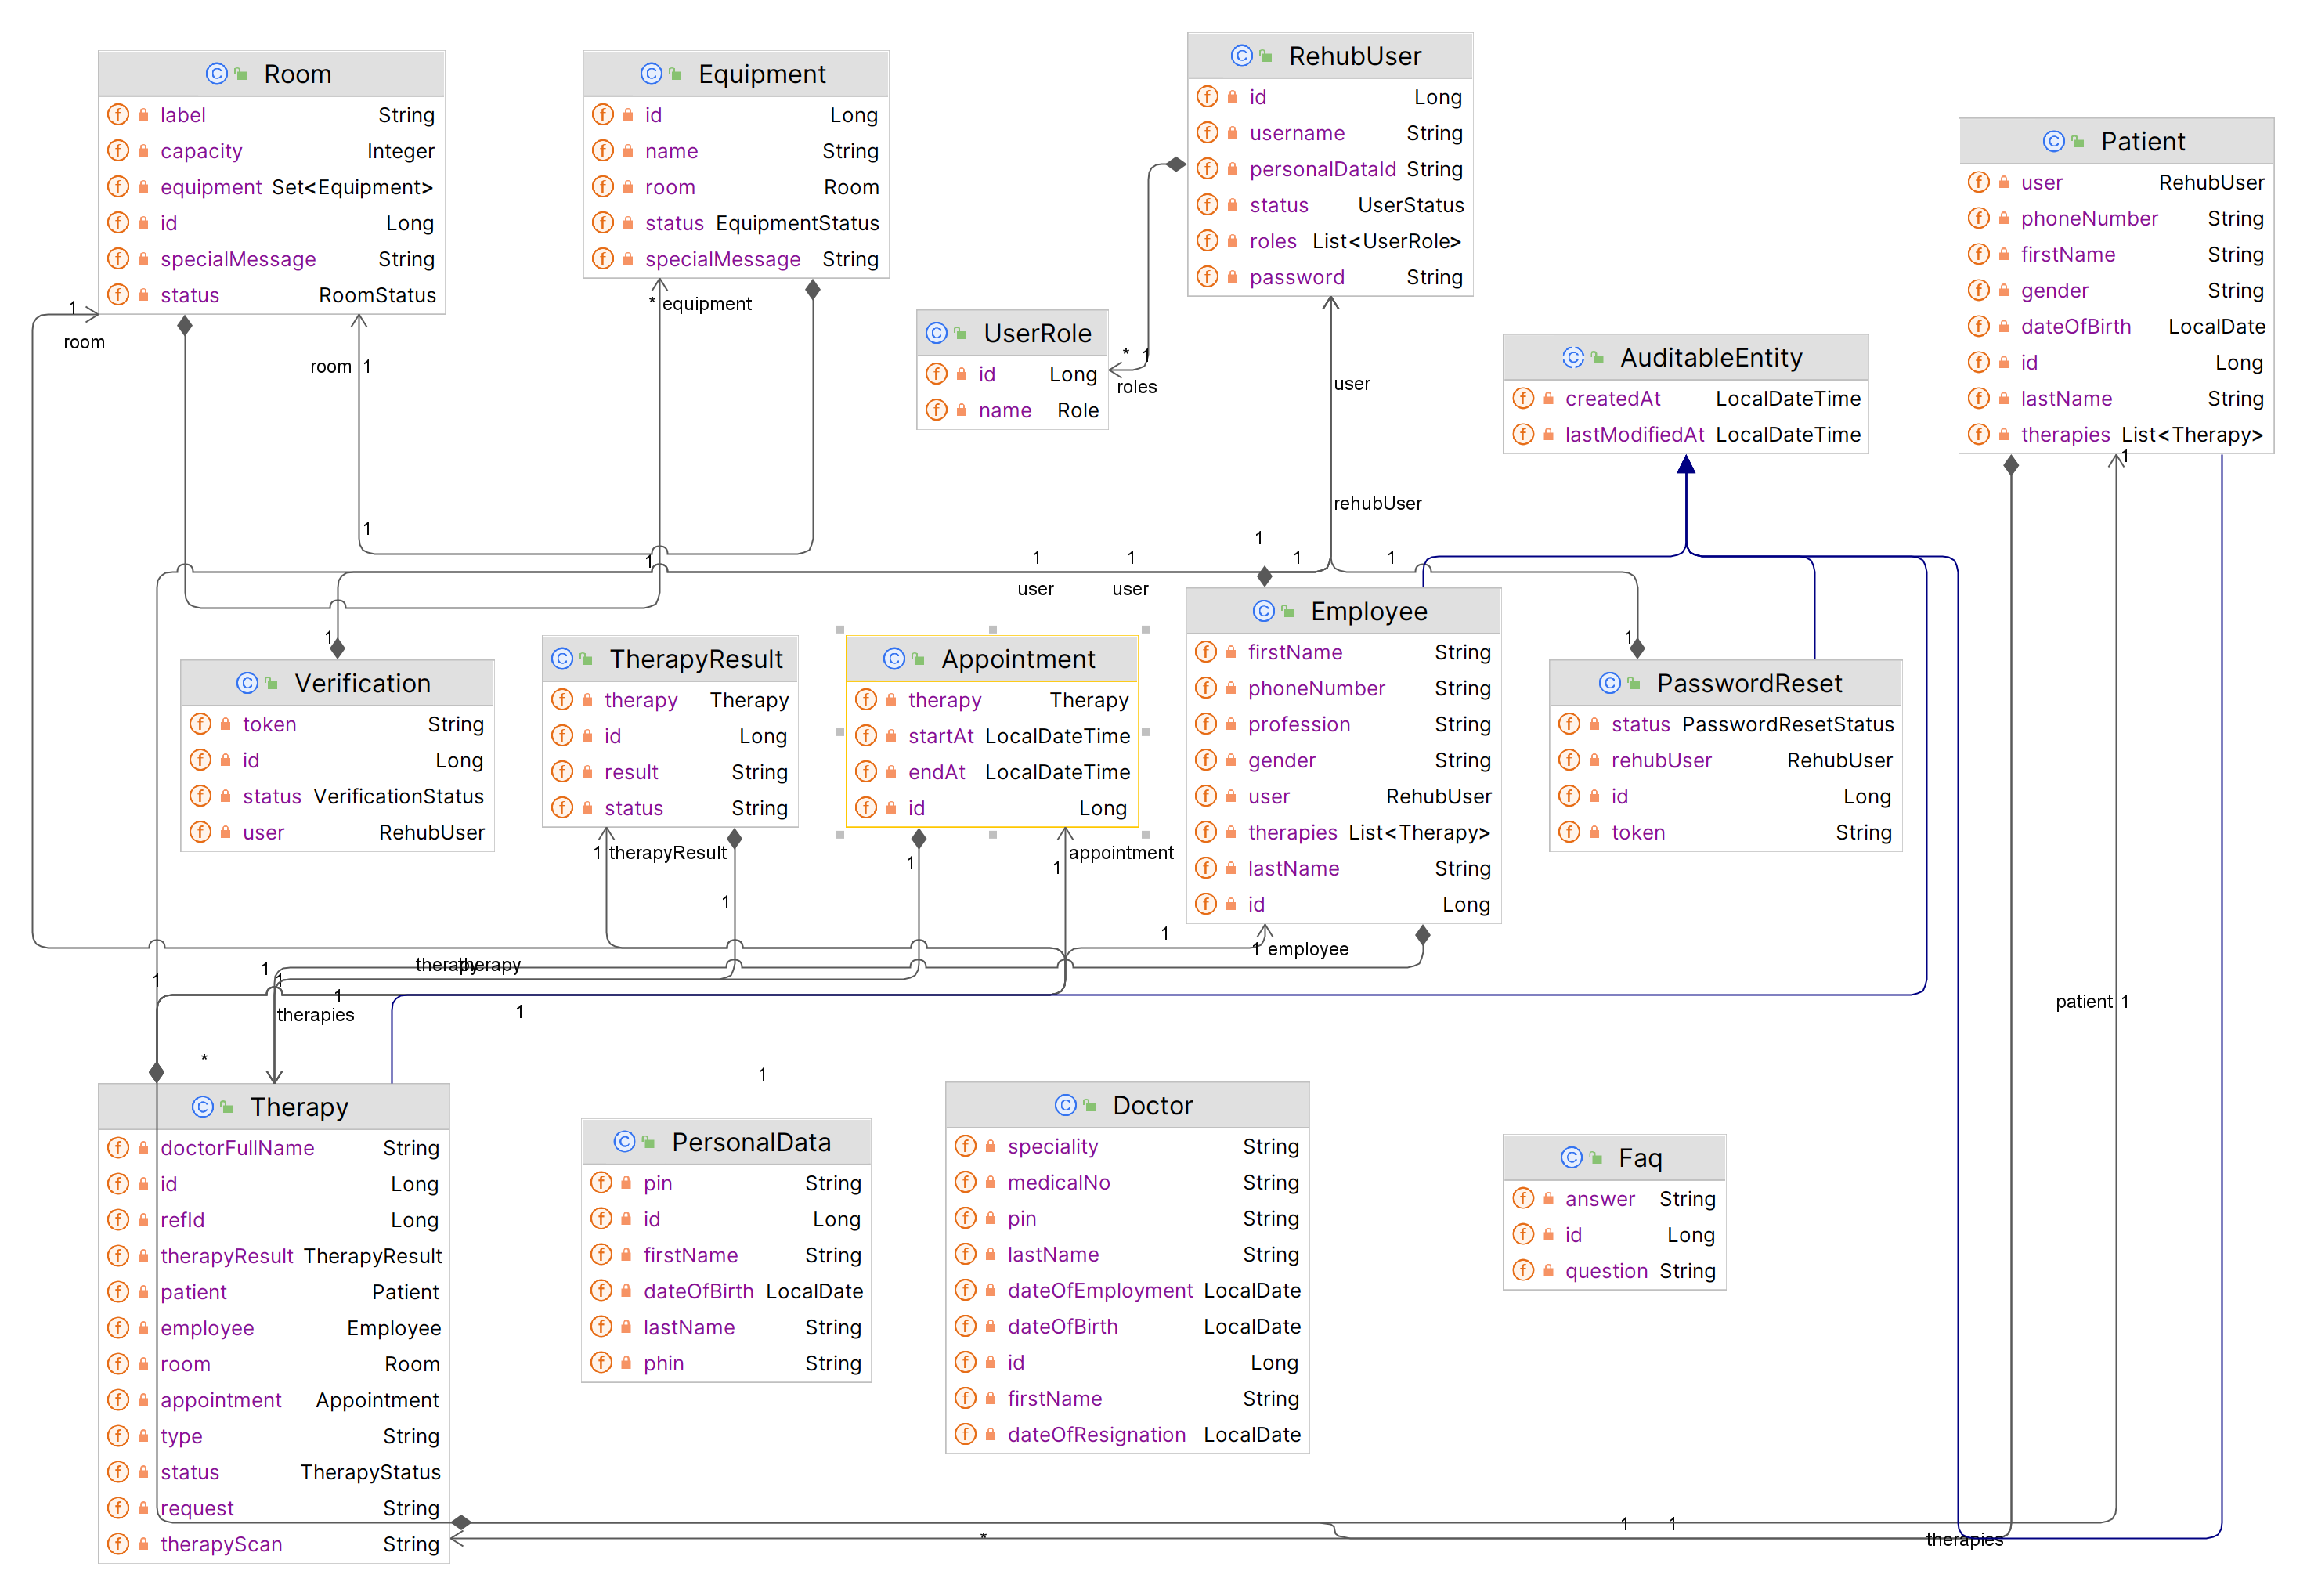
\includegraphics[scale=0.15]{dijagrami/Entity.png}
	\centering
	\caption{Dijagram razreda (Model)}
	\label{fig:EntityClassDiagram}
\end{figure}

\begin{figure}[H]
	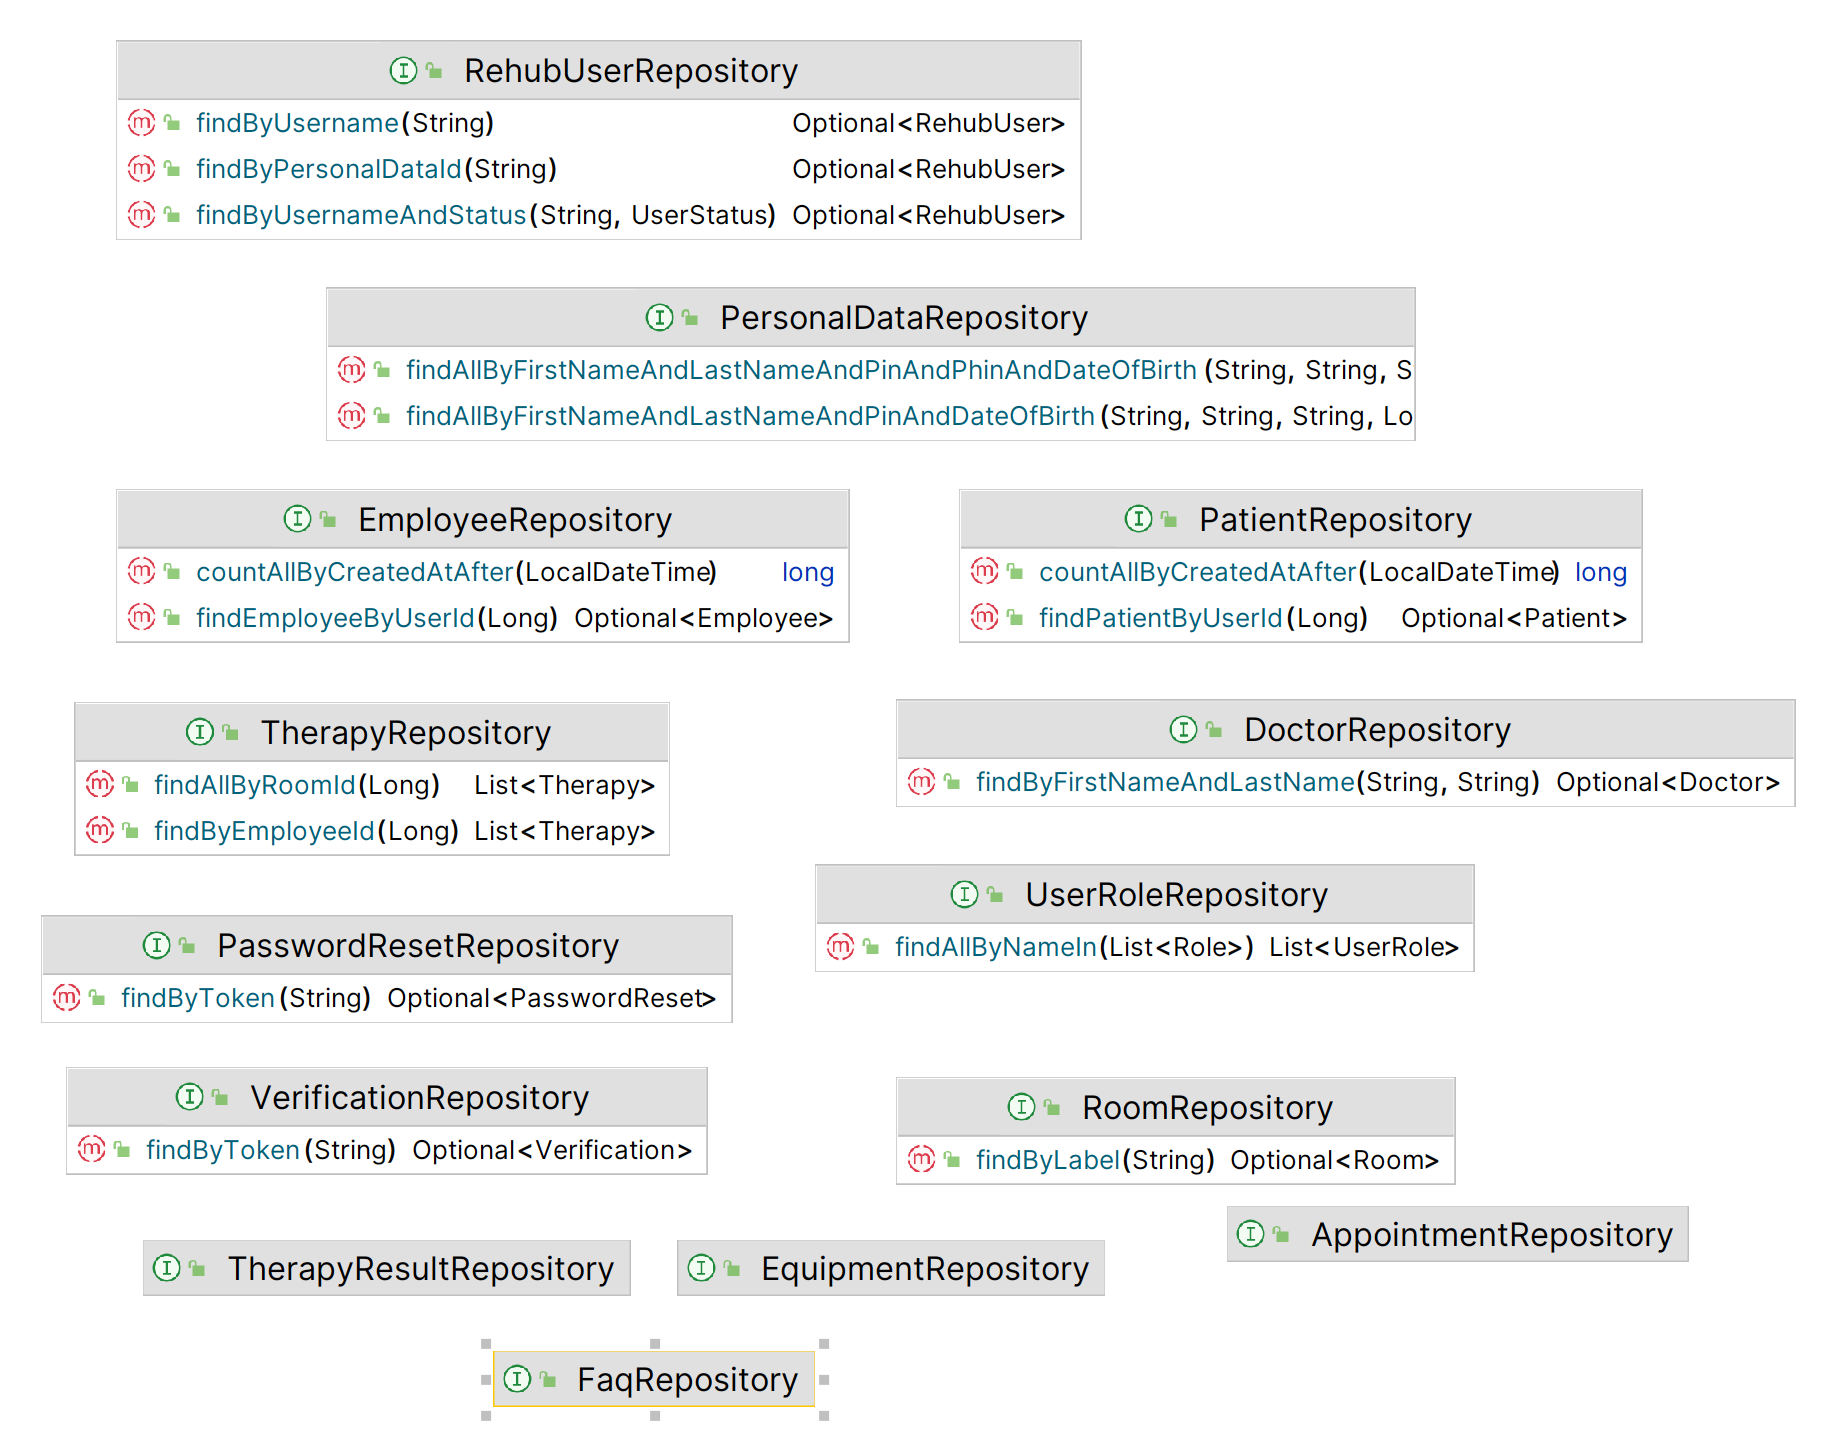
\includegraphics[scale=0.22]{dijagrami/Repository.png}
	\centering
	\caption{Dijagram razreda (Repository)}
	\label{fig:RepositoryClassDiagram}
\end{figure}

\begin{figure}[H]
	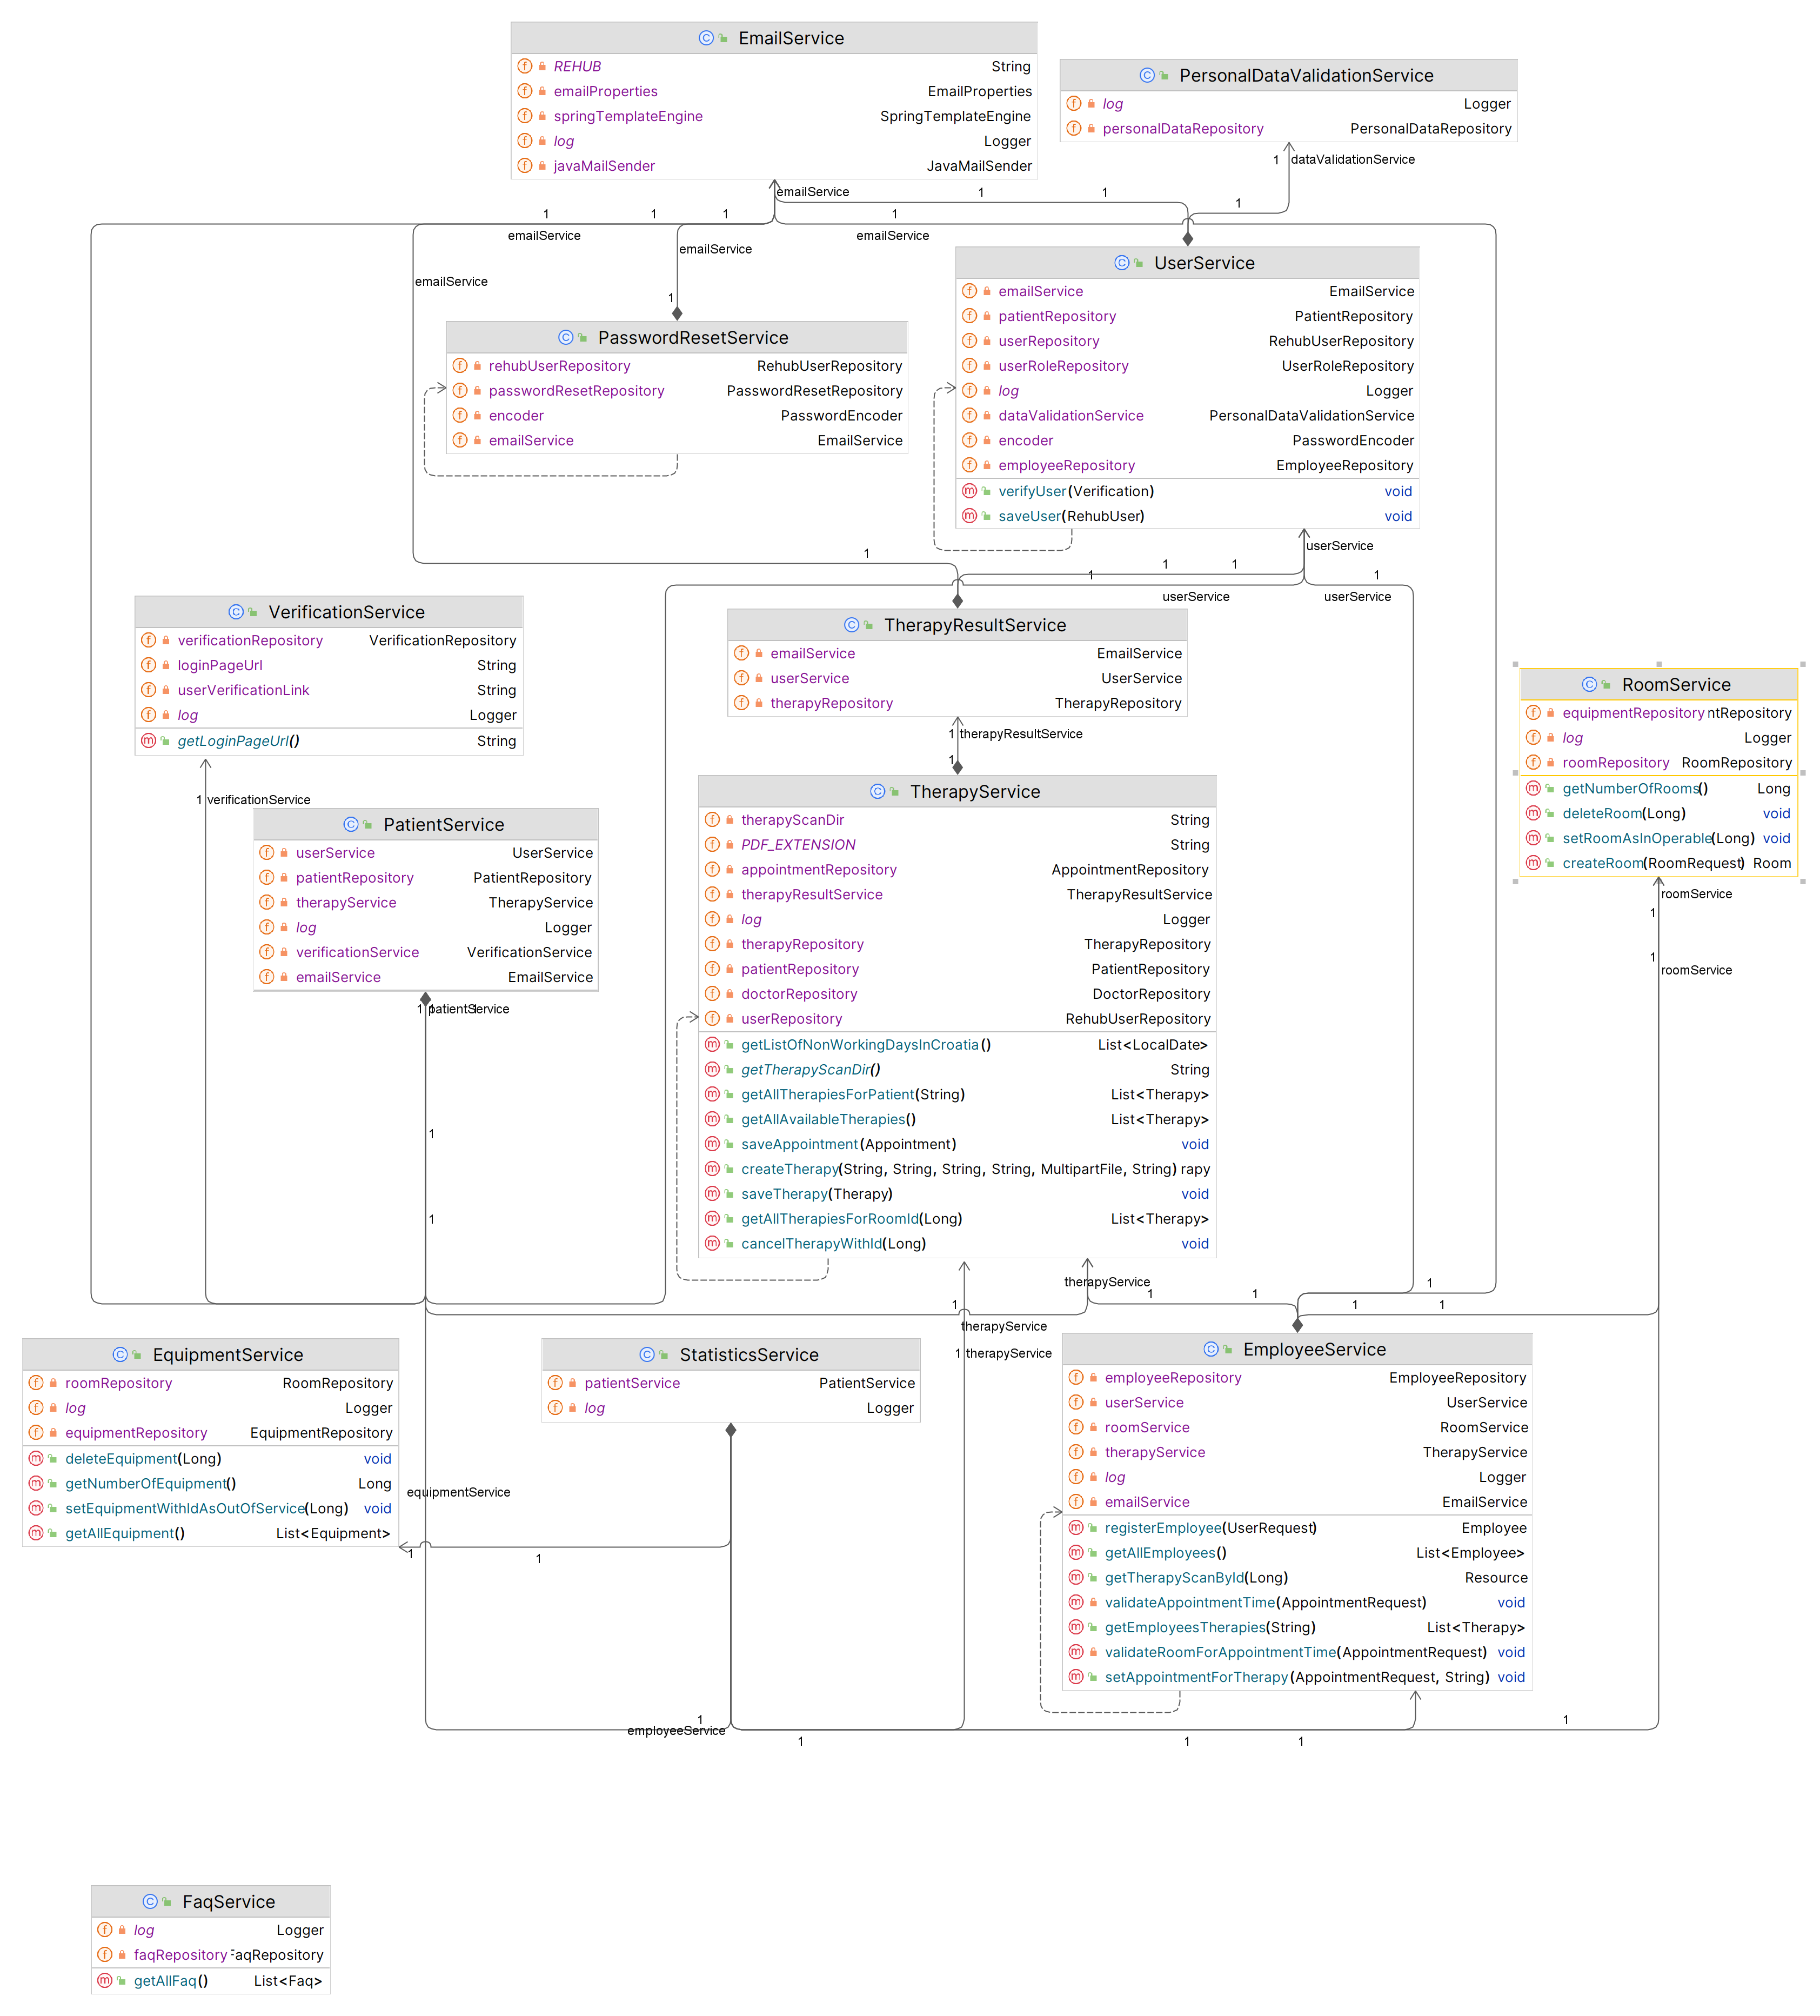
\includegraphics[scale=0.1]{dijagrami/Service.png}
	\centering
	\caption{Dijagram razreda (Service)}
	\label{fig:ServiceClassDiagram}
\end{figure}

\begin{figure}[H]
	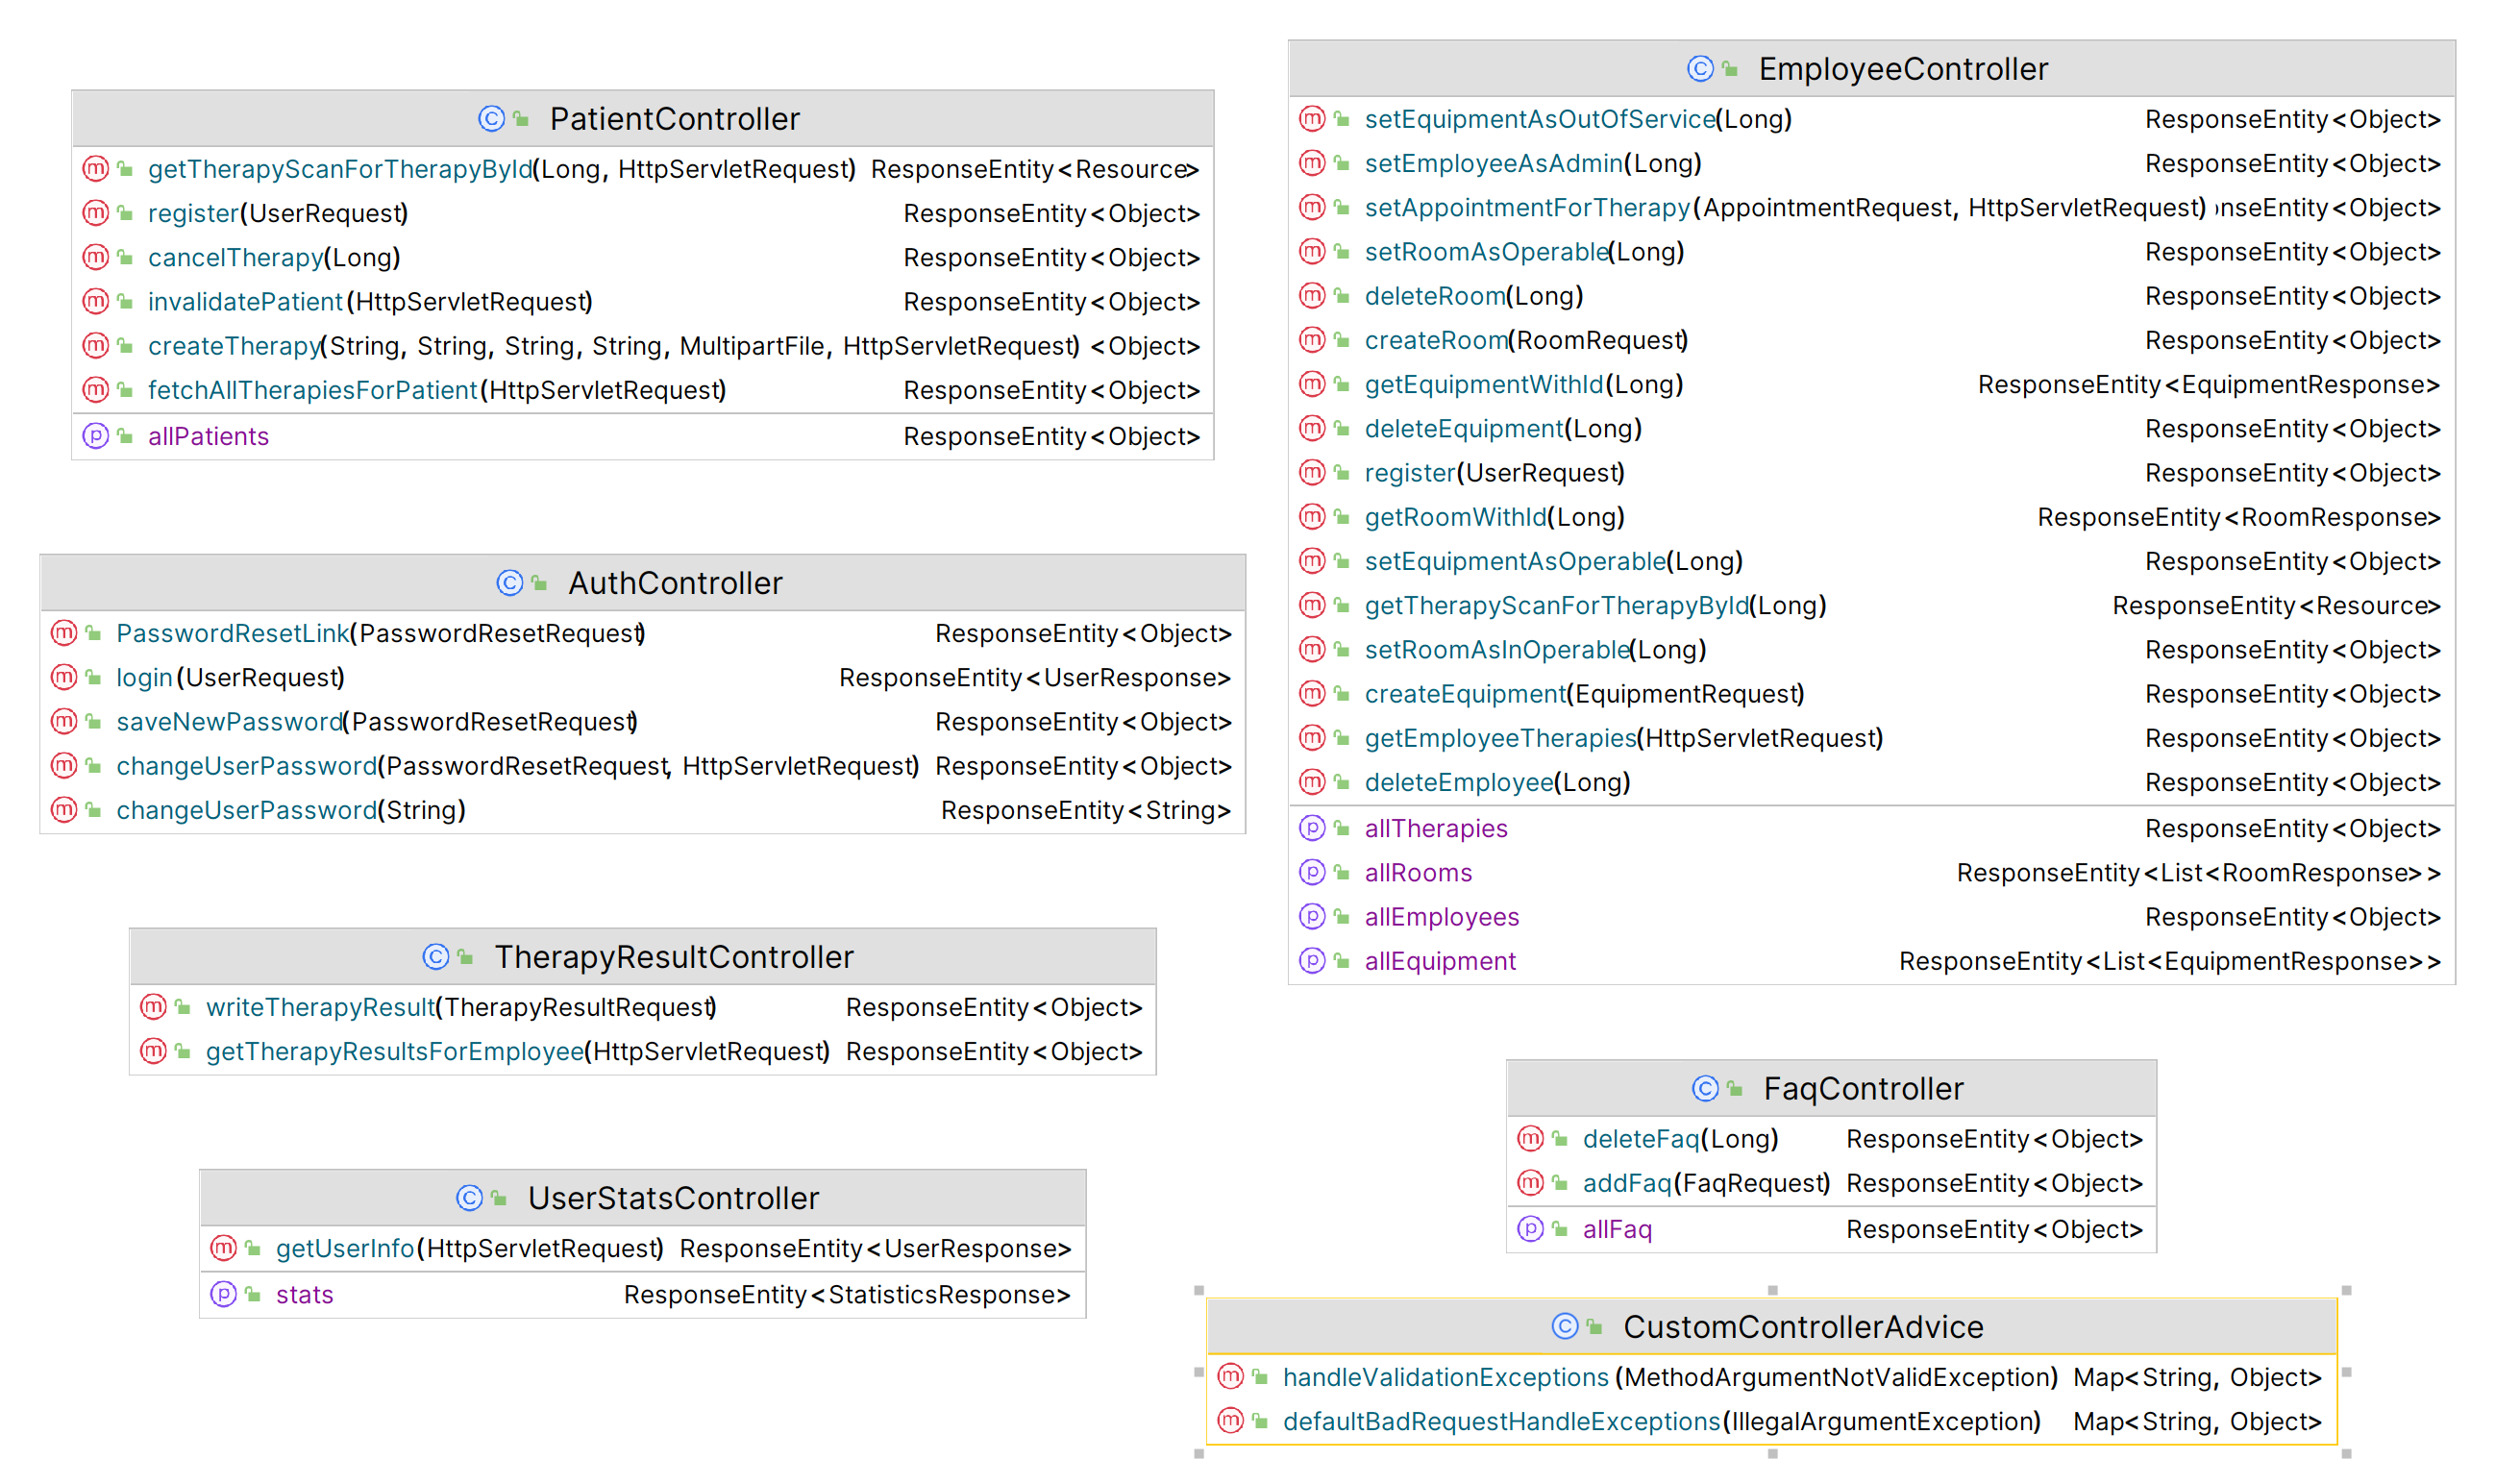
\includegraphics[scale=0.15]{dijagrami/Controller.png}
	\centering
	\caption{Dijagram razreda (Controller)}
	\label{fig:ControllerClassDiagram}
\end{figure}

\begin{figure}[H]
	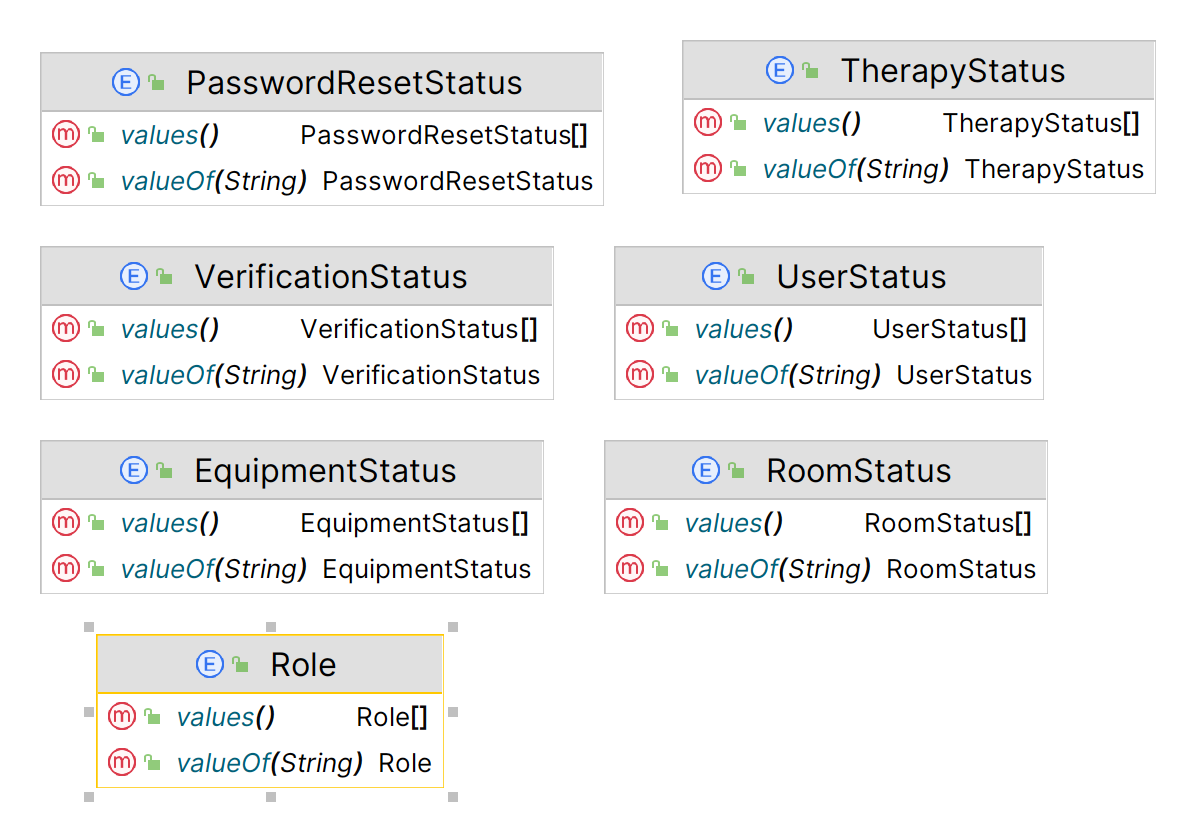
\includegraphics[scale=0.2]{dijagrami/Enum.png}
	\centering
	\caption{Dijagram enumeracija (Model)}
	\label{fig:EnumClassDiagram}
\end{figure}

\begin{figure}[H]
	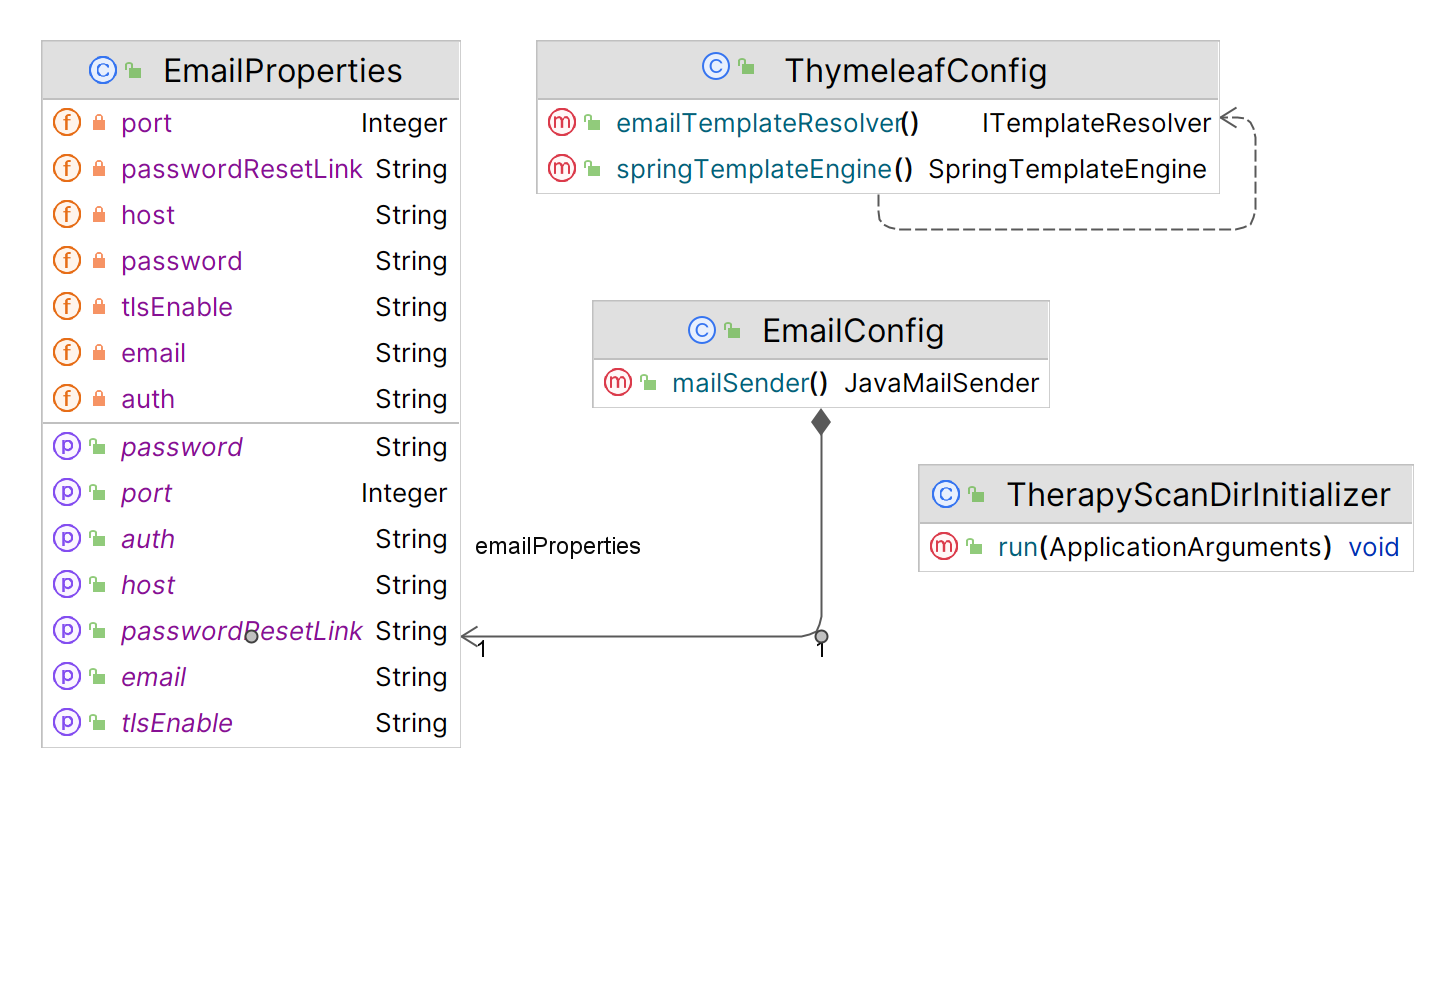
\includegraphics[scale=0.18]{dijagrami/Config.png}
	\centering
	\caption{Dijagram razreda (Config)}
	\label{fig:ConfigClassDiagram}
\end{figure}

\begin{figure}[H]
	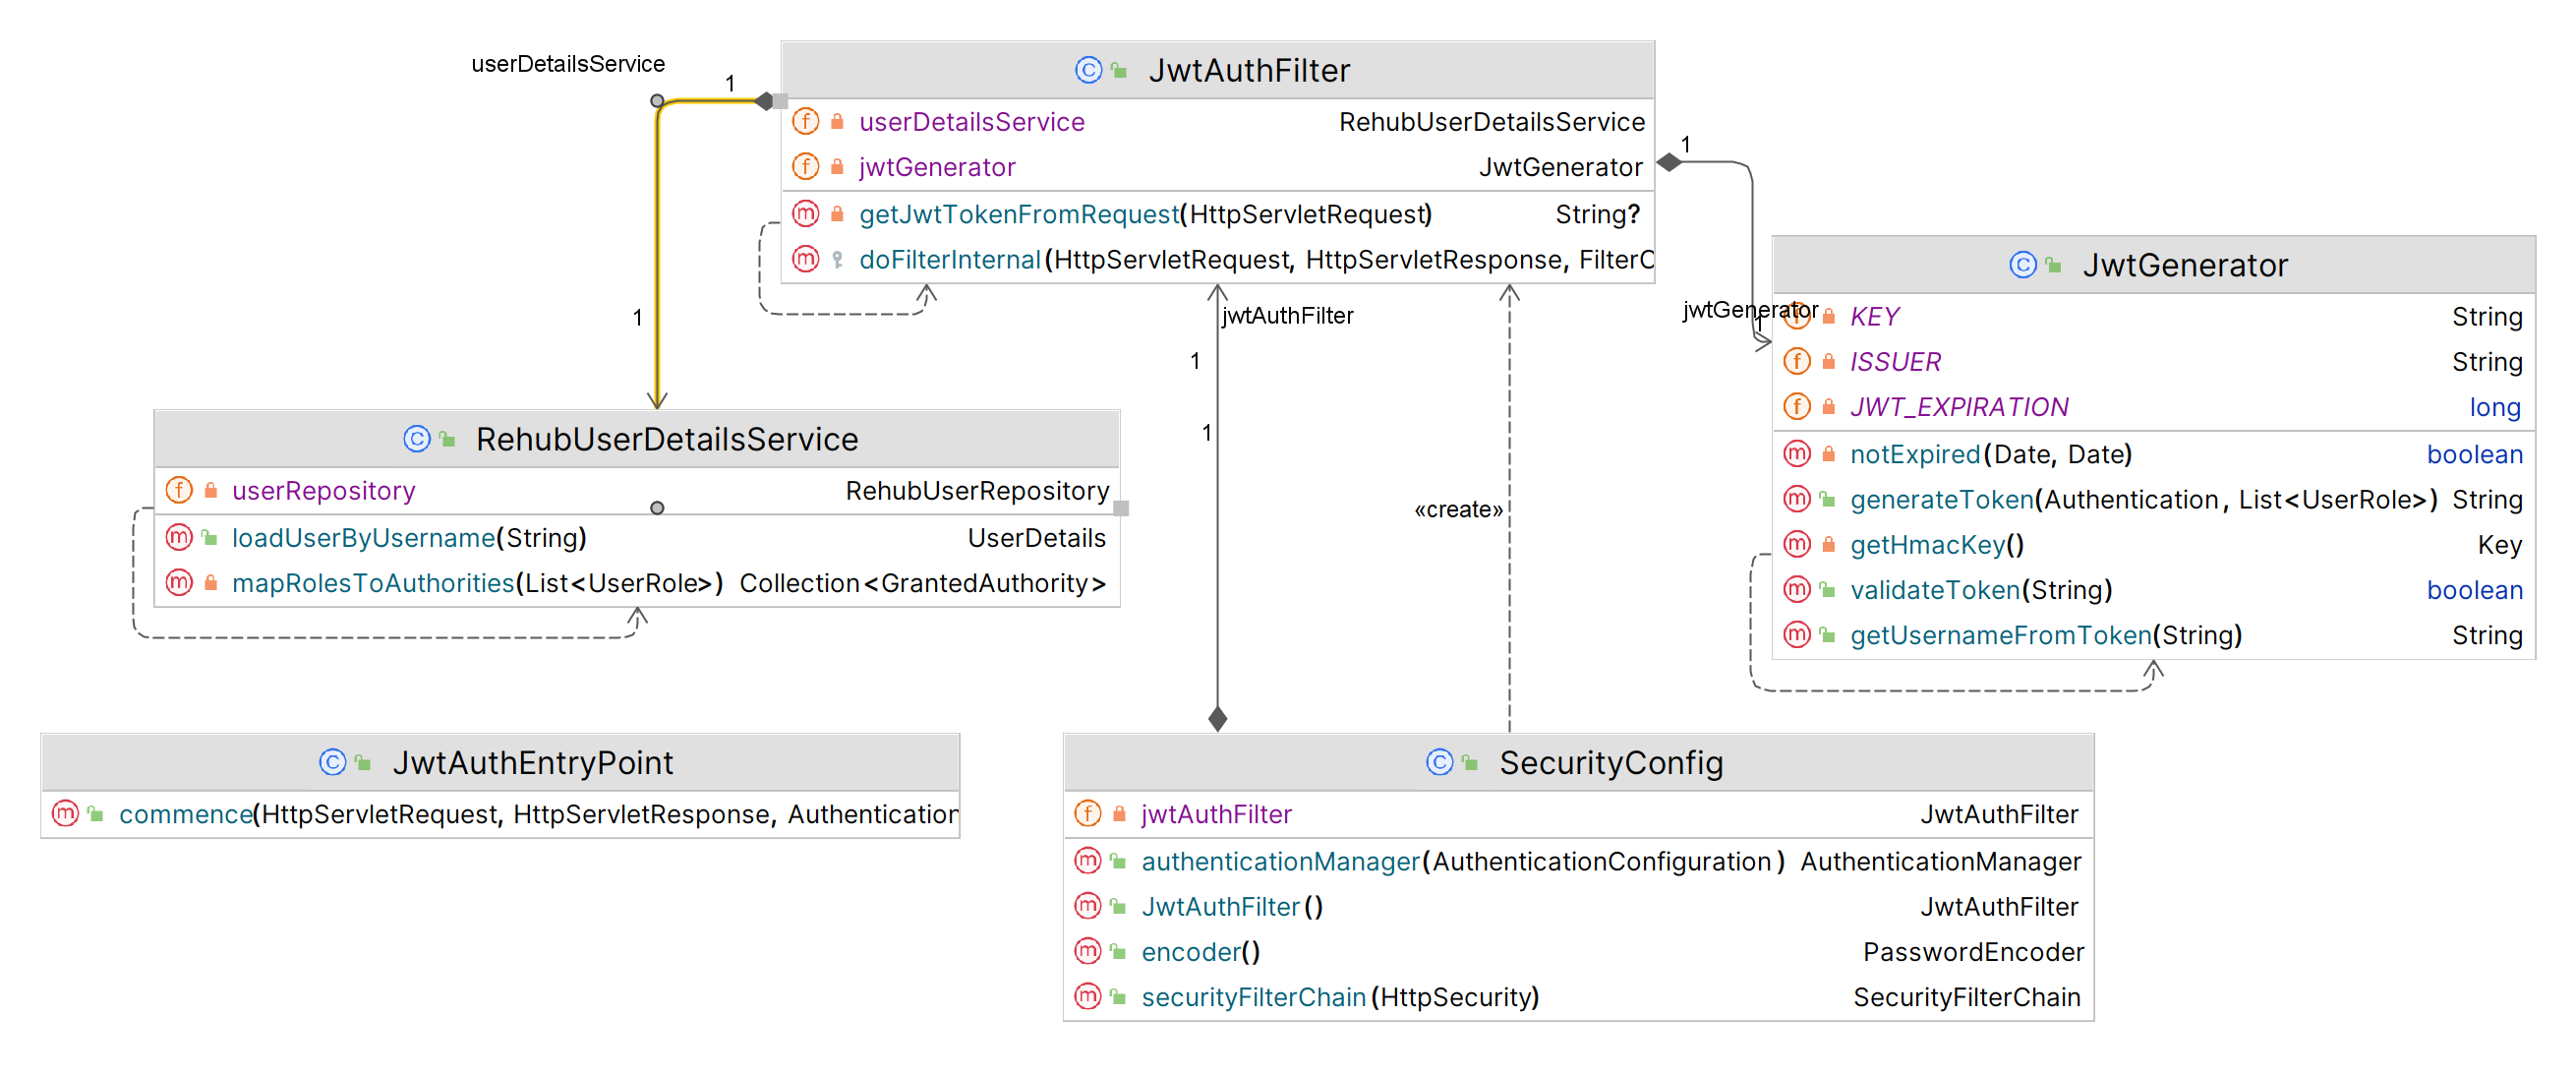
\includegraphics[scale=0.18]{dijagrami/Security.png}
	\centering
	\caption{Dijagram razreda (Security)}
	\label{fig:SecurityClassDiagram}
\end{figure}

\begin{figure}[H]
	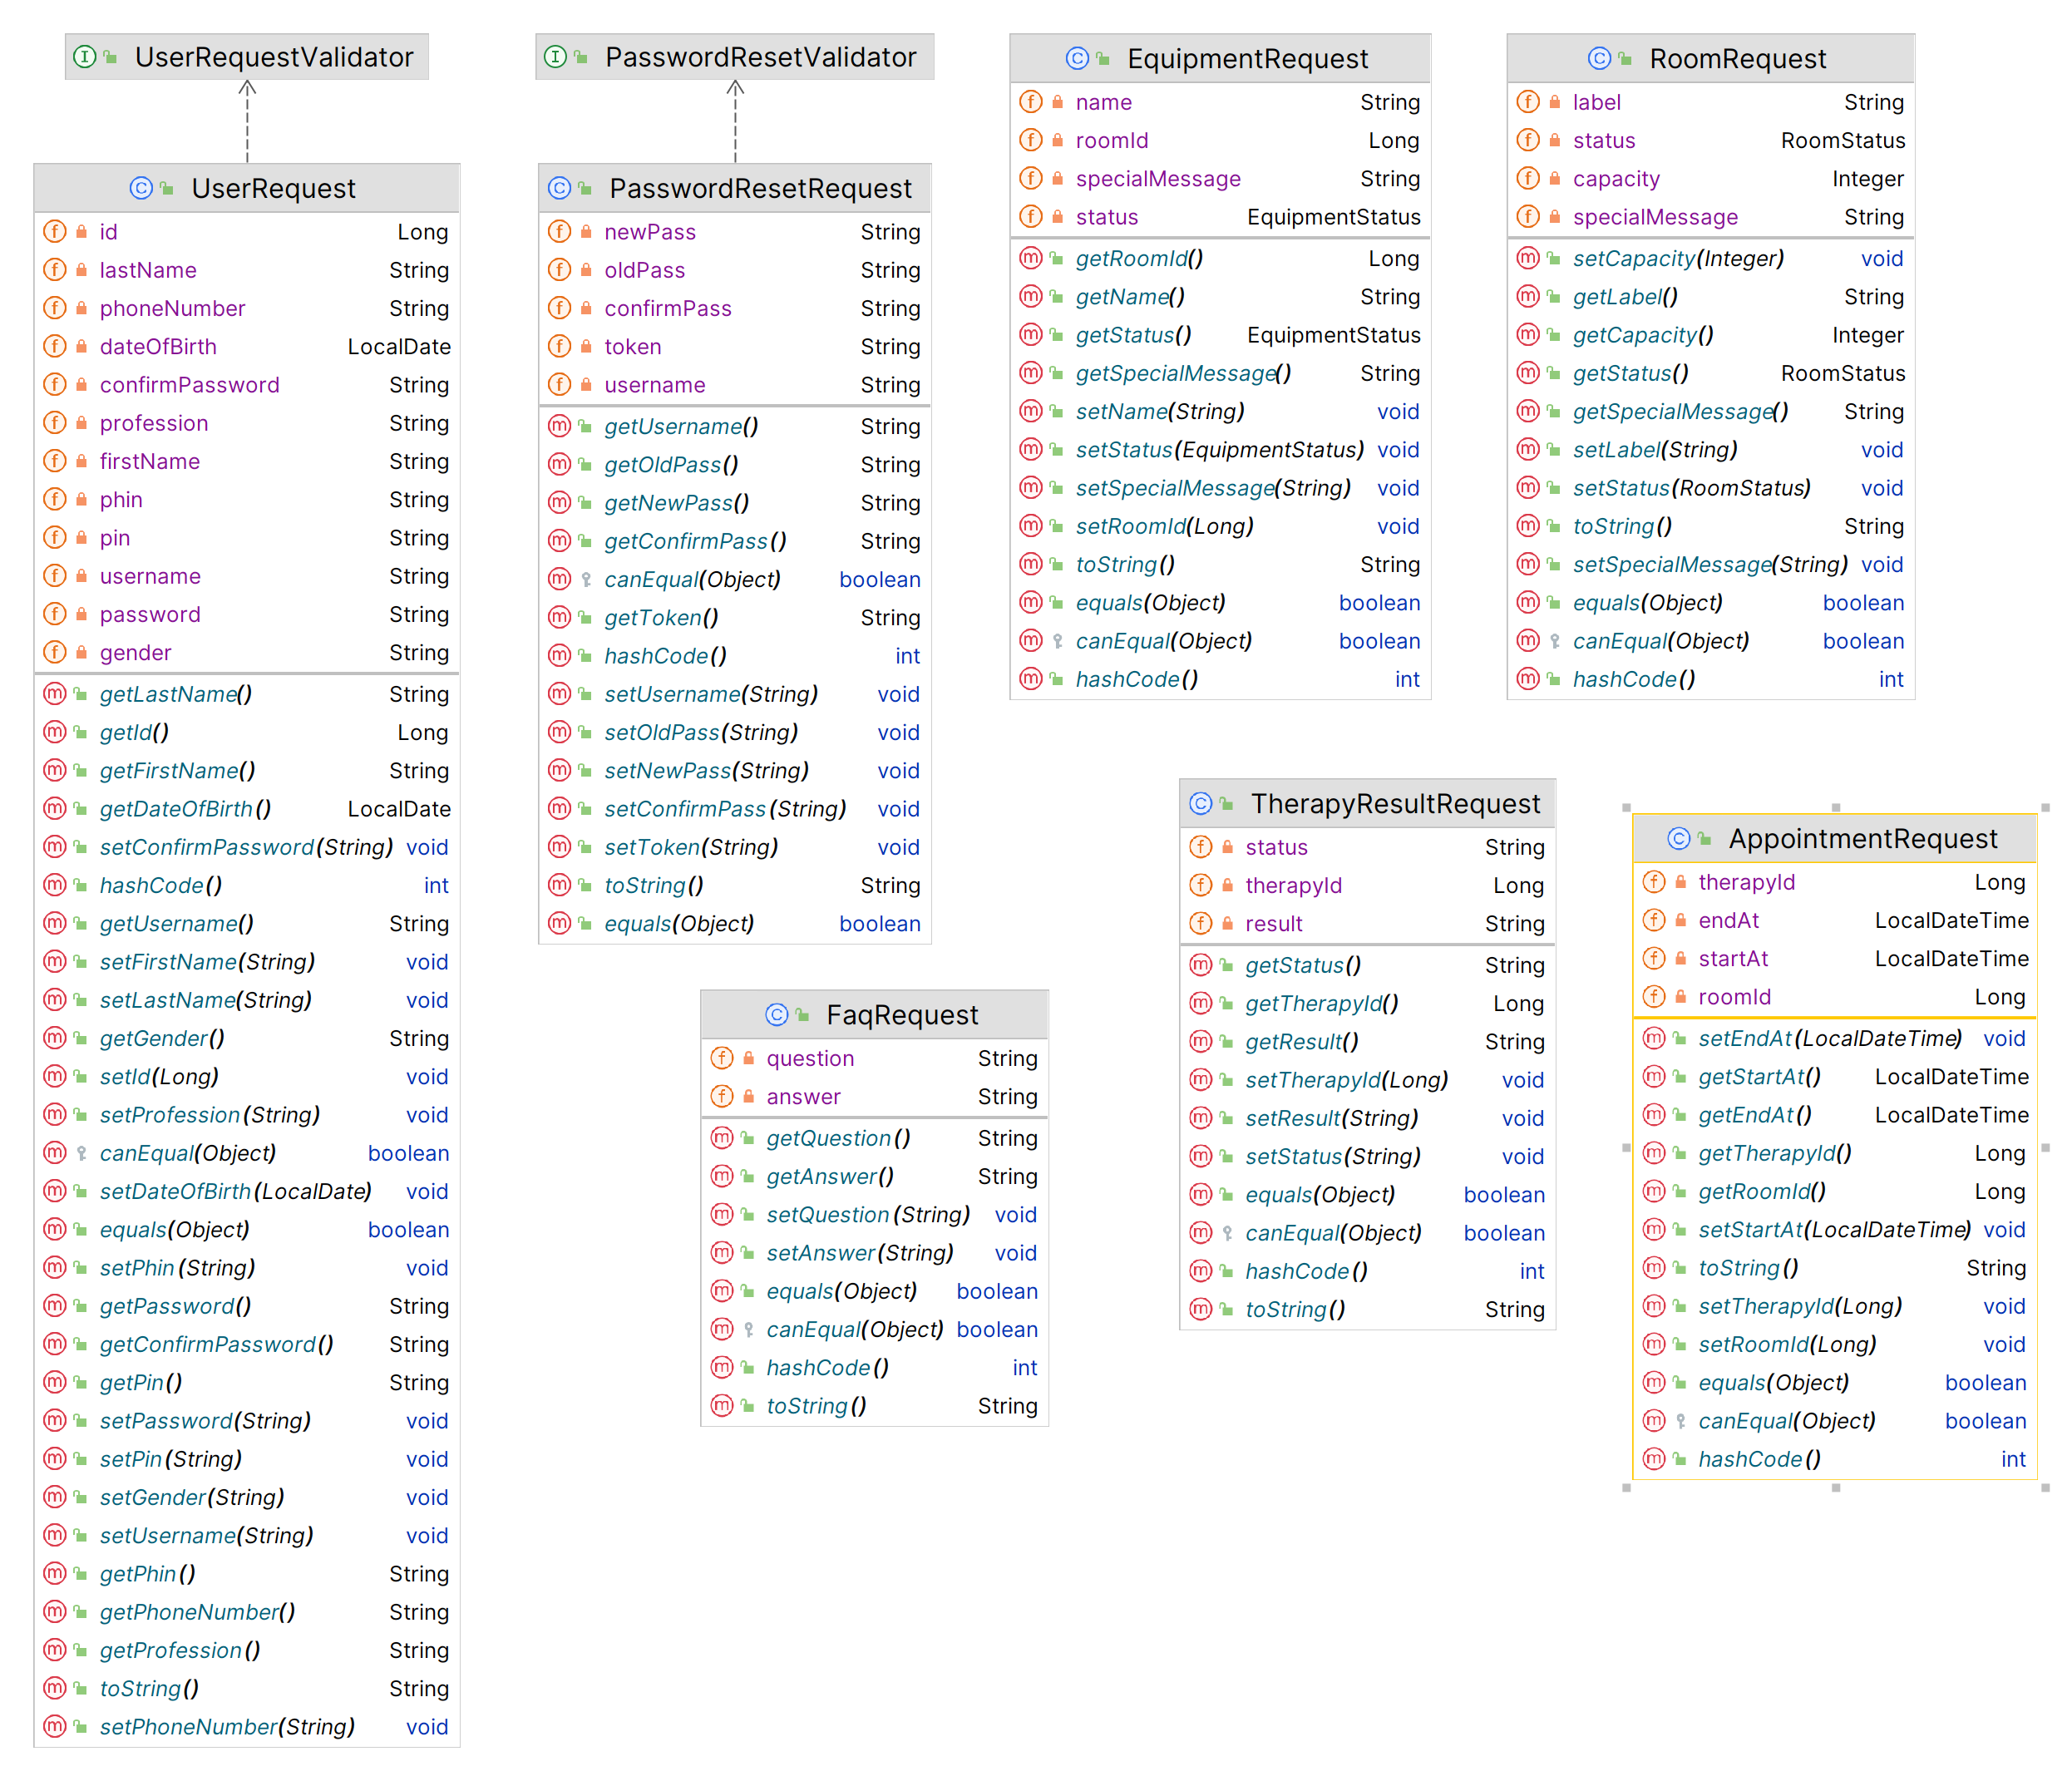
\includegraphics[scale=0.18]{dijagrami/Request.png}
	\centering
	\caption{Dijagram razreda (Request)}
	\label{fig:RequestClassDiagrams}
\end{figure}

\begin{figure}[H]
	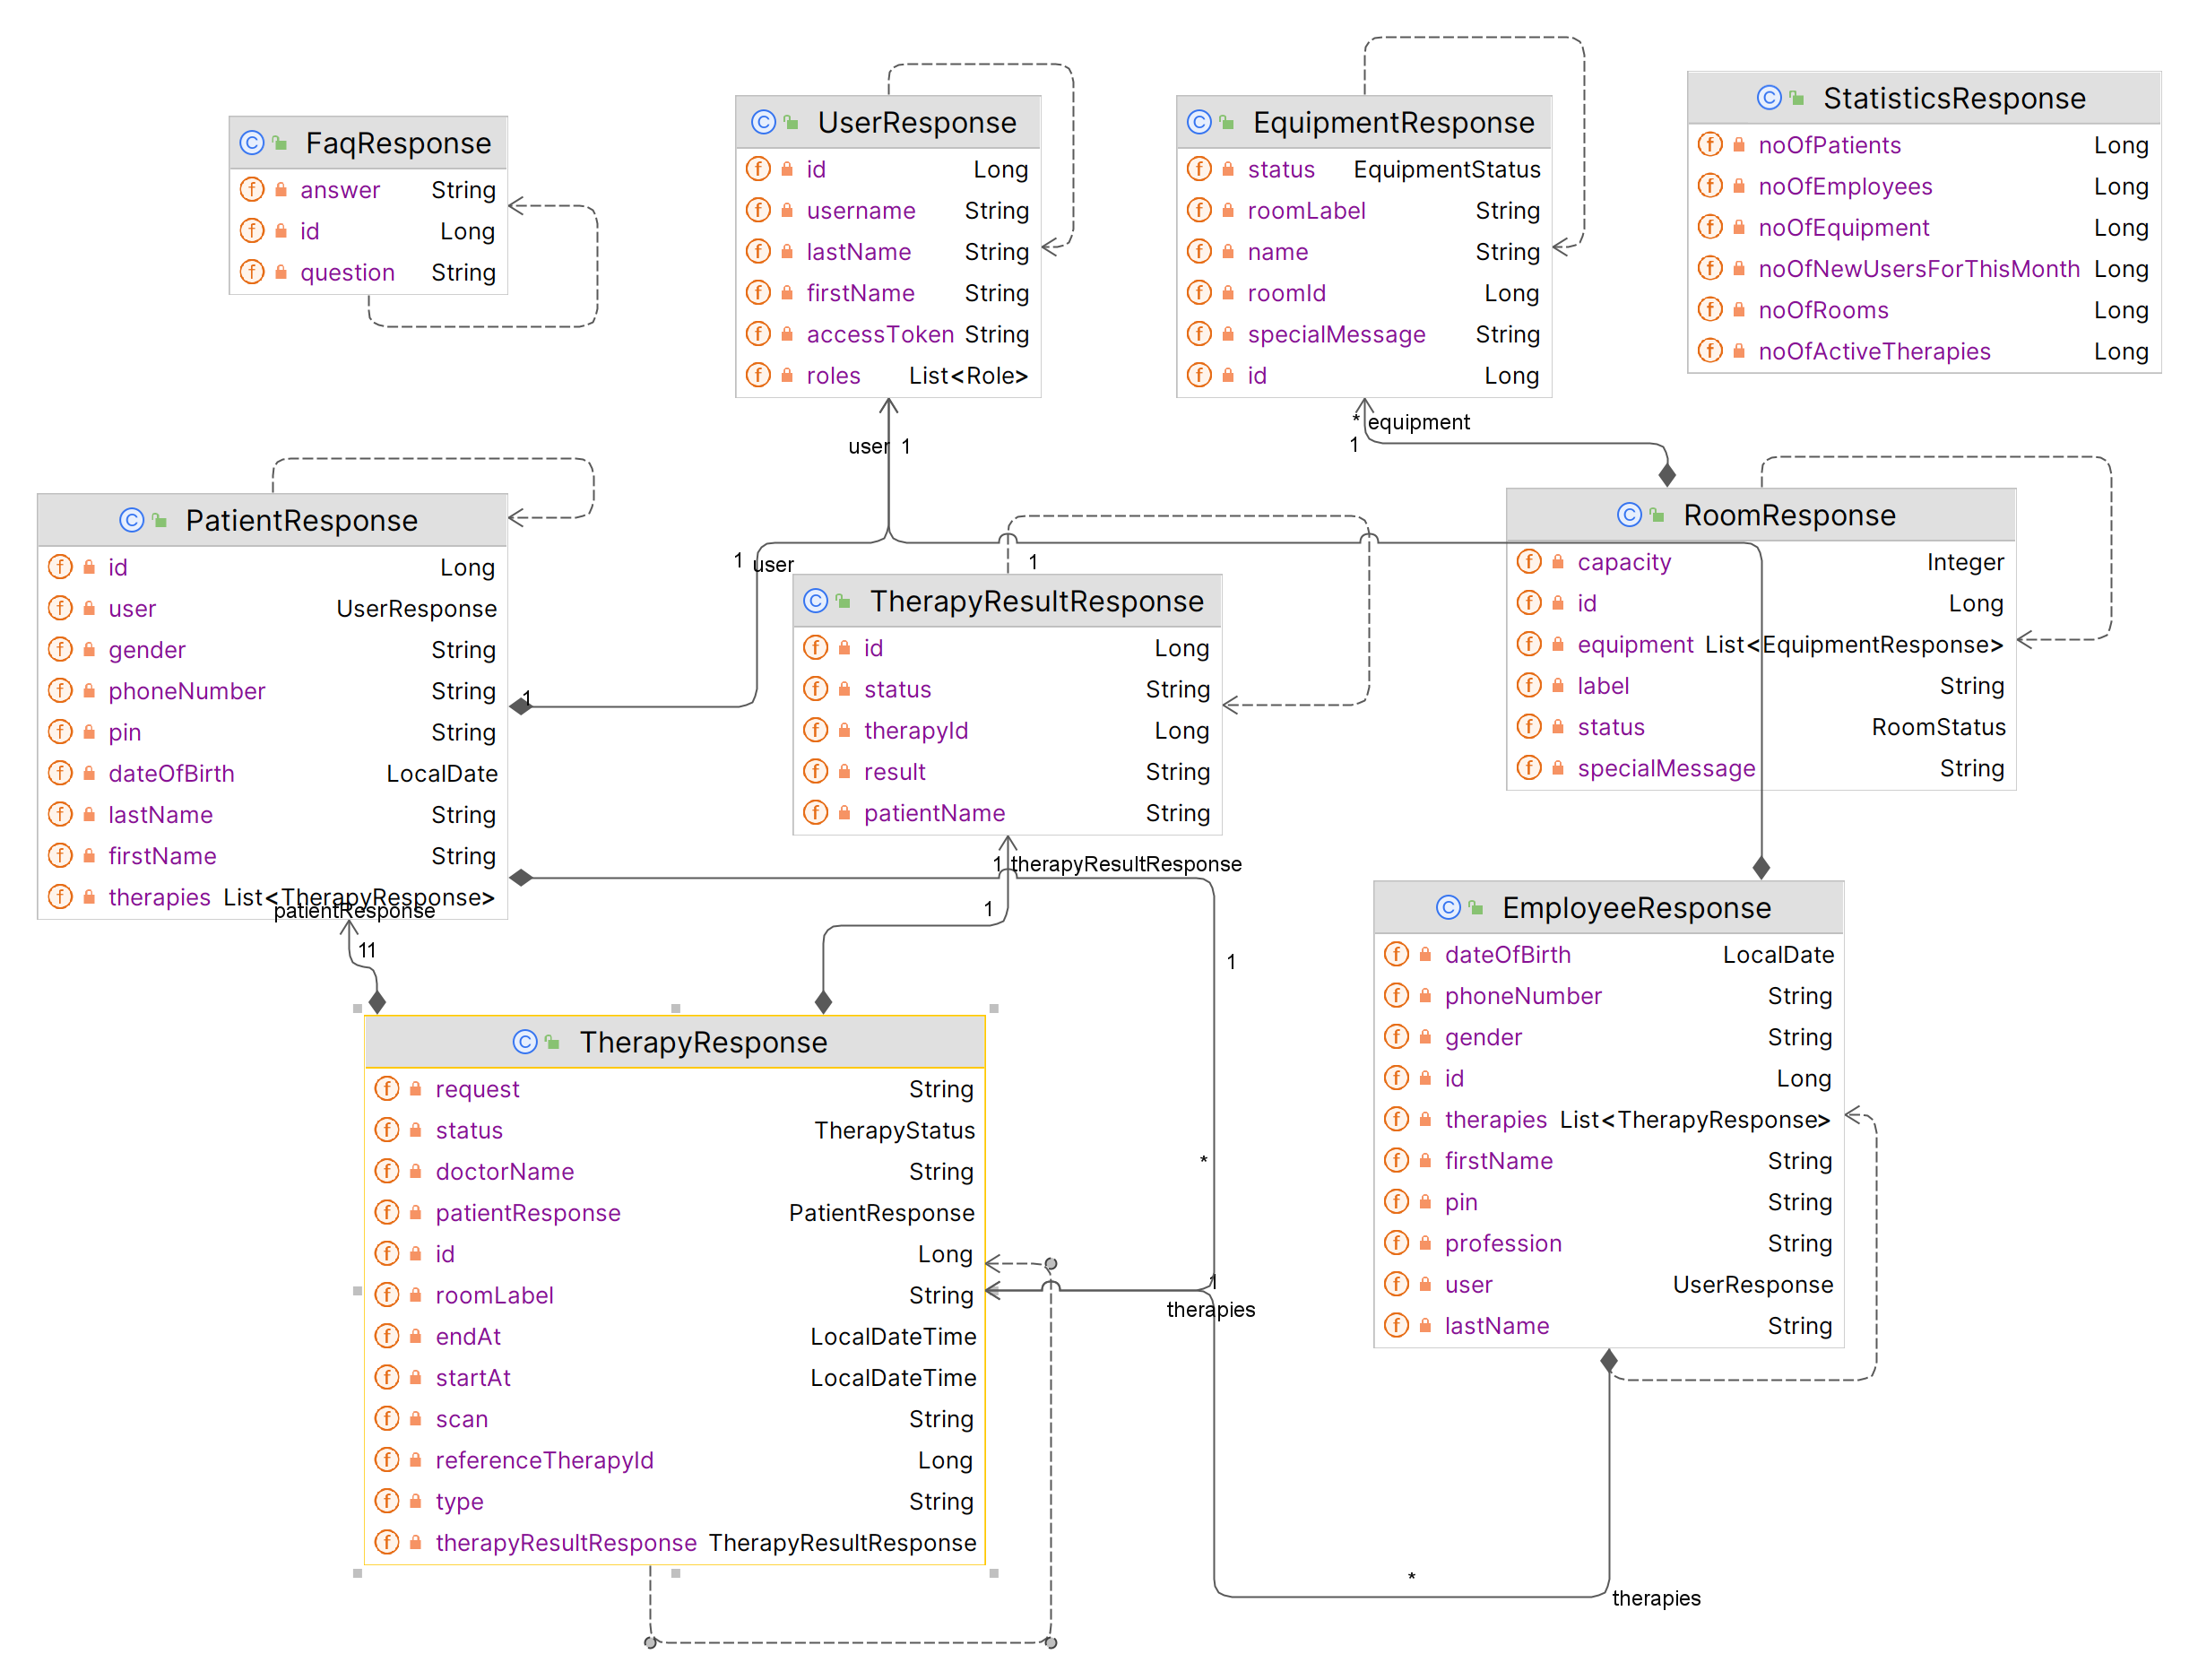
\includegraphics[scale=0.16]{dijagrami/Response.png}
	\centering
	\caption{Dijagram razreda (Response)}
	\label{fig:ResponseClassDiagram}
\end{figure}



\eject

\section{Dijagram stanja}

Dijagram stanja prikazuje stanja objekta te prijelaze iz jednog stanja u drugo temeljene na dogadajima. Prilikom pokretanja aplikacije dolazi se na početnu stranicu (eng.Home page). Neregistrirani korisnik ima mogućcnost registracije i pregled kontakta i učestalih pitanja bez registracije

Registrirani korisnik na svojem početnom zaslonu nakon prijave može kliknuti na svoj profil gdje vidi svoje podatke, također na profilnoj stranici može deaktivirati račun i promjenit lozinku. Klikom na Dodaj novi termin korisnik se može prijaviti za termin koji može i naknadno otkazati.

Zaposlenik na svojem zaslonu može kao i korisnik kliknut na svoj profil gdje vidi svoje podatke i mjenja lozinku. Može davati termine i sobe pristiglim prijavama kao i pregledavati gotove termine te pisati rezultate terapije.

Superadmin ima uvid u statistiku, ima popis svih pacijenta i osoblja. Može dodavati, brisati osoblje te im dati uloge admina. Također ima popis svih soba i opreme koje može brisati i dodavati ili staviti da nisu u funkciji.

\begin{figure}[H]
	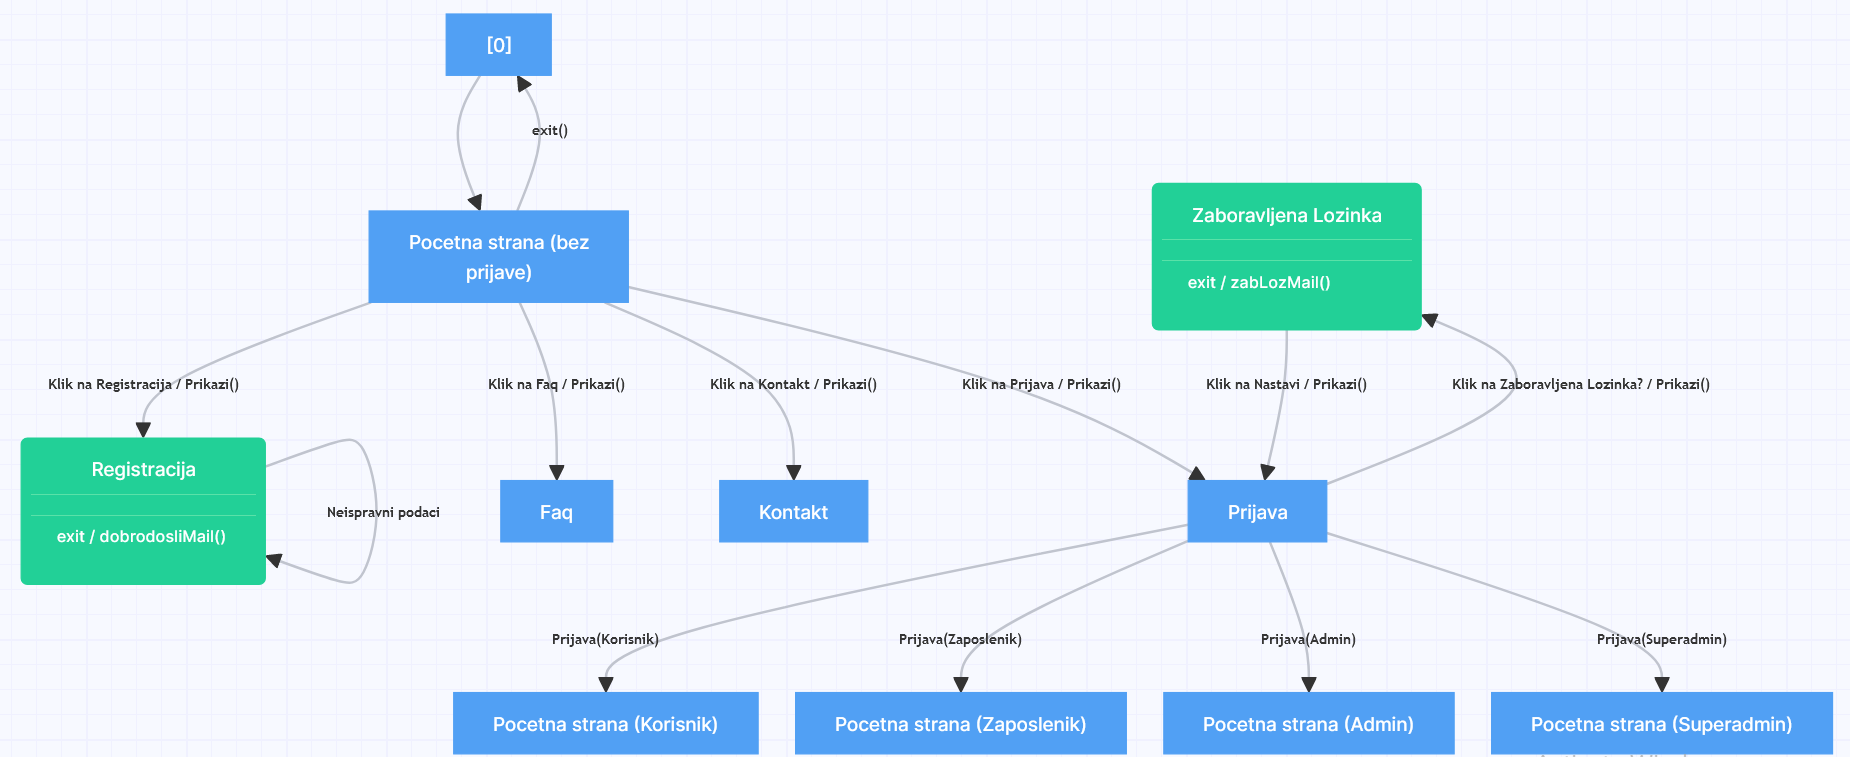
\includegraphics[scale=0.4]{dijagrami/bezprijave.png}
	\centering
	\caption{Dijagram stanja (neprijavljeni korisnik)}
	\label{fig:bezprijave}
\end{figure}

\begin{figure}[H]
	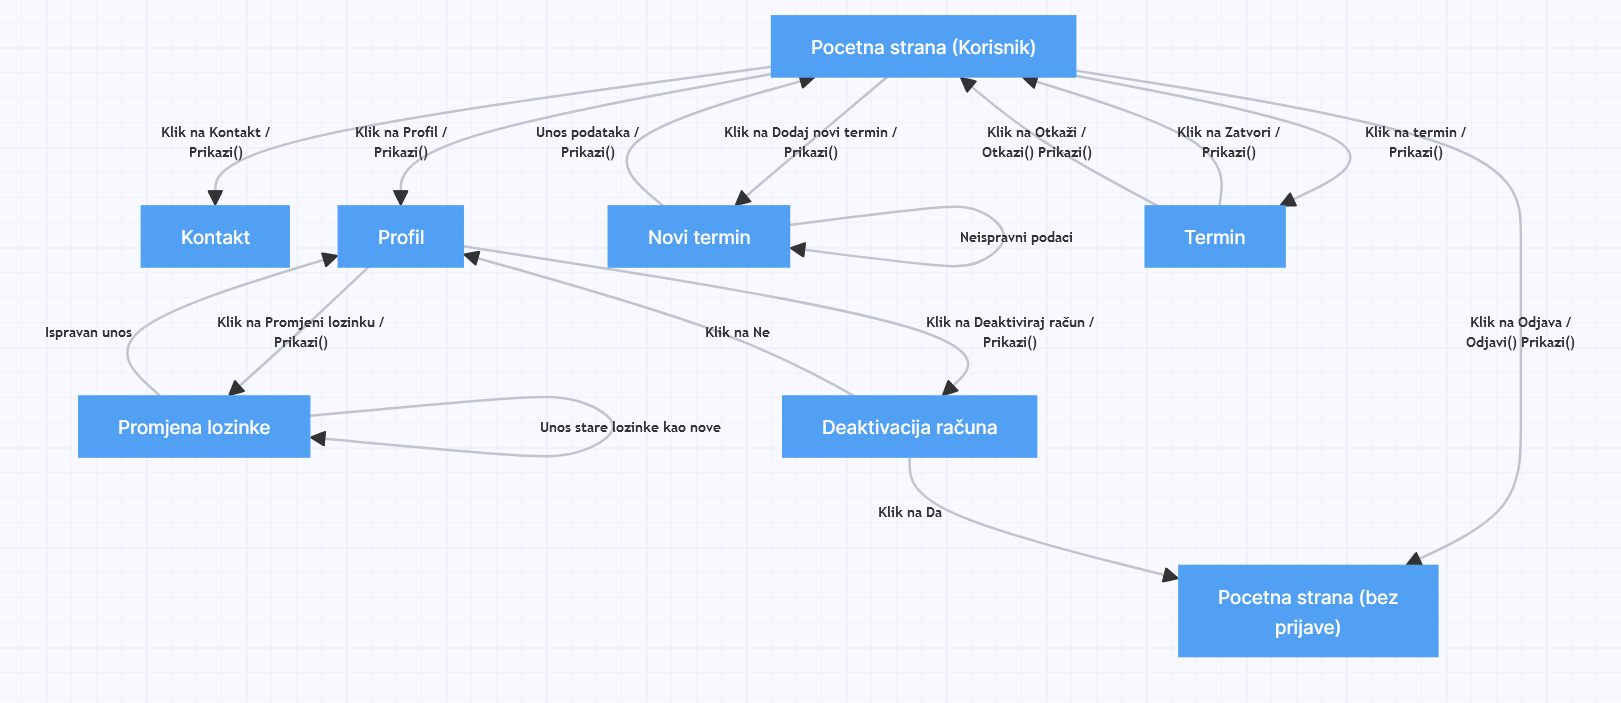
\includegraphics[scale=0.4]{dijagrami/korisnik.png}
	\centering
	\caption{Dijagram stanja (prijavljeni korisnik)}
	\label{fig:korisnik}
\end{figure}

\begin{figure}[H]
	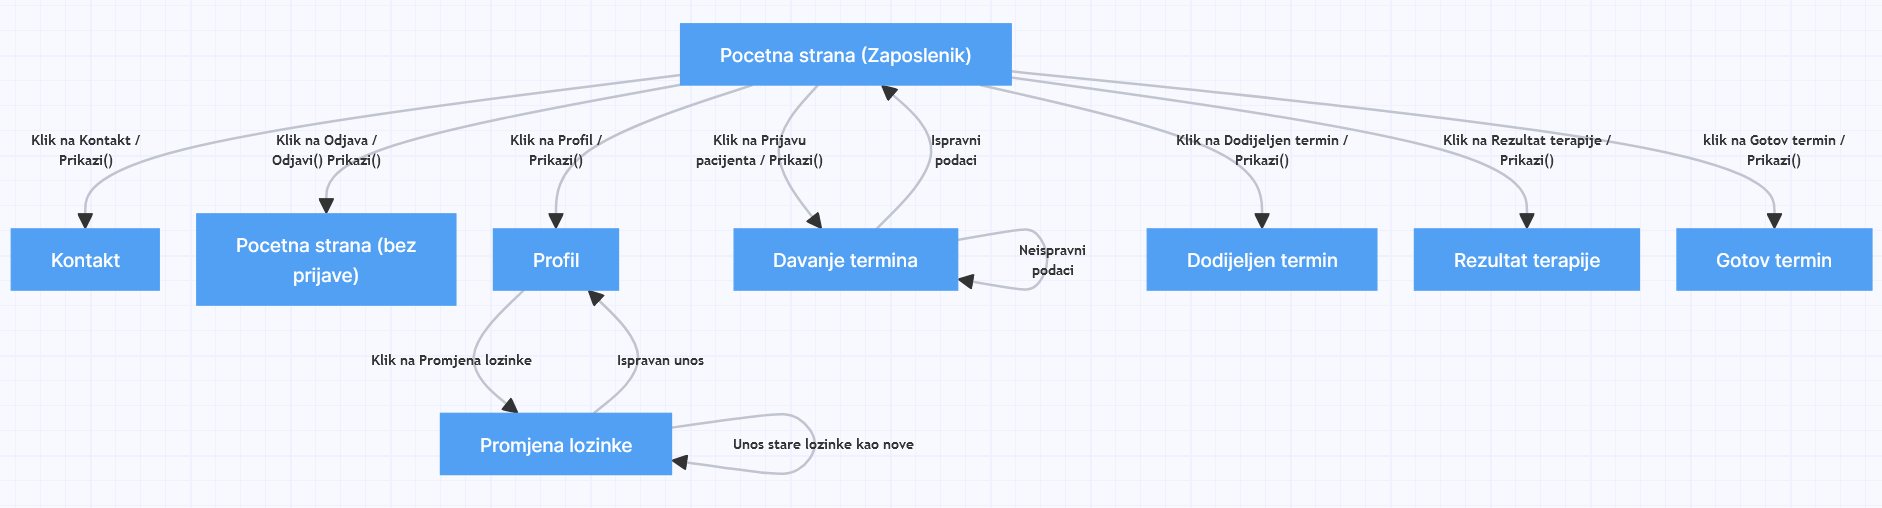
\includegraphics[scale=0.4]{dijagrami/zaposlenik.png}
	\centering
	\caption{Dijagram stanja (zaposlenik)}
	\label{fig:zaposlenik}
\end{figure}

\begin{figure}[H]
	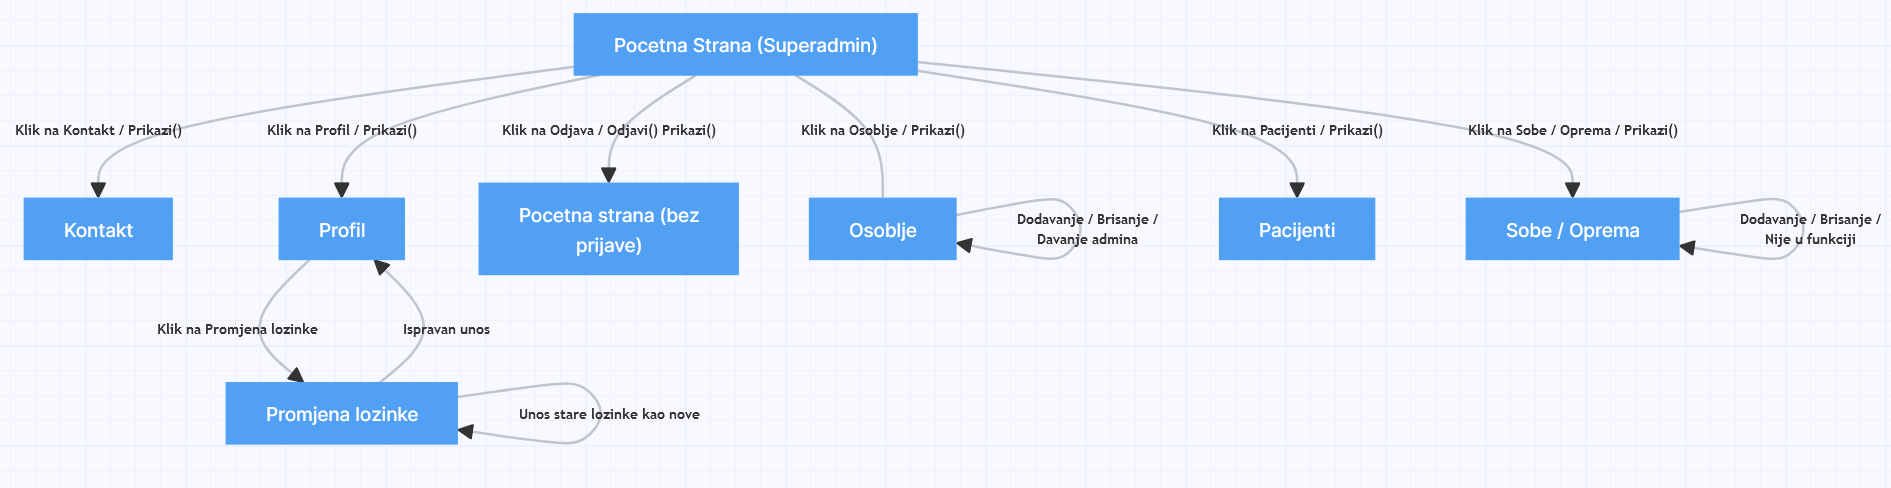
\includegraphics[scale=0.4]{dijagrami/superadmin.png}
	\centering
	\caption{Dijagram stanja (superadmin)}
	\label{fig:superadmin}
\end{figure}

\eject 

\section{Dijagram aktivnosti}

Pacijent započinje proces prijavom u sustav putem web-aplikacije, unoseći svoje korisničke podatke. Web-aplikacija šalje upit za provjeru tih podataka bazi podataka, koja zatim vraća rezultat. Ako su uneseni podaci neispravni, pacijent mora ponovno unijeti podatke, inače mu se prikazuje stranica za pacijente. Nakon uspješne prijave, pacijent odabire stvaranje nove terapije, što rezultira prikazom forme za unos podataka o bolesti i liječniku koji je dao uputnicu. Ponovno se šalje upit za provjeru tih podataka bazi, a ako su neispravni, pacijent ponovno unosi informacije; inače, liječnik prima zahtjev za terapijom i unosi podatke o datumu, vremenu i sobi za terapiju. Web-aplikacija ponovno šalje upit za provjeru podataka bazi, a u slučaju neispravnih podataka, liječnik ih ponovno unosi. U suprotnom, web-aplikacija šalje e-mail o potvrdi terapije i prikazuje stranicu za pacijenta s dodijeljenim terminom. Nakon toga, podaci o zahtjevu za terapijom spremaju se u sustav.

\begin{figure}[H]
	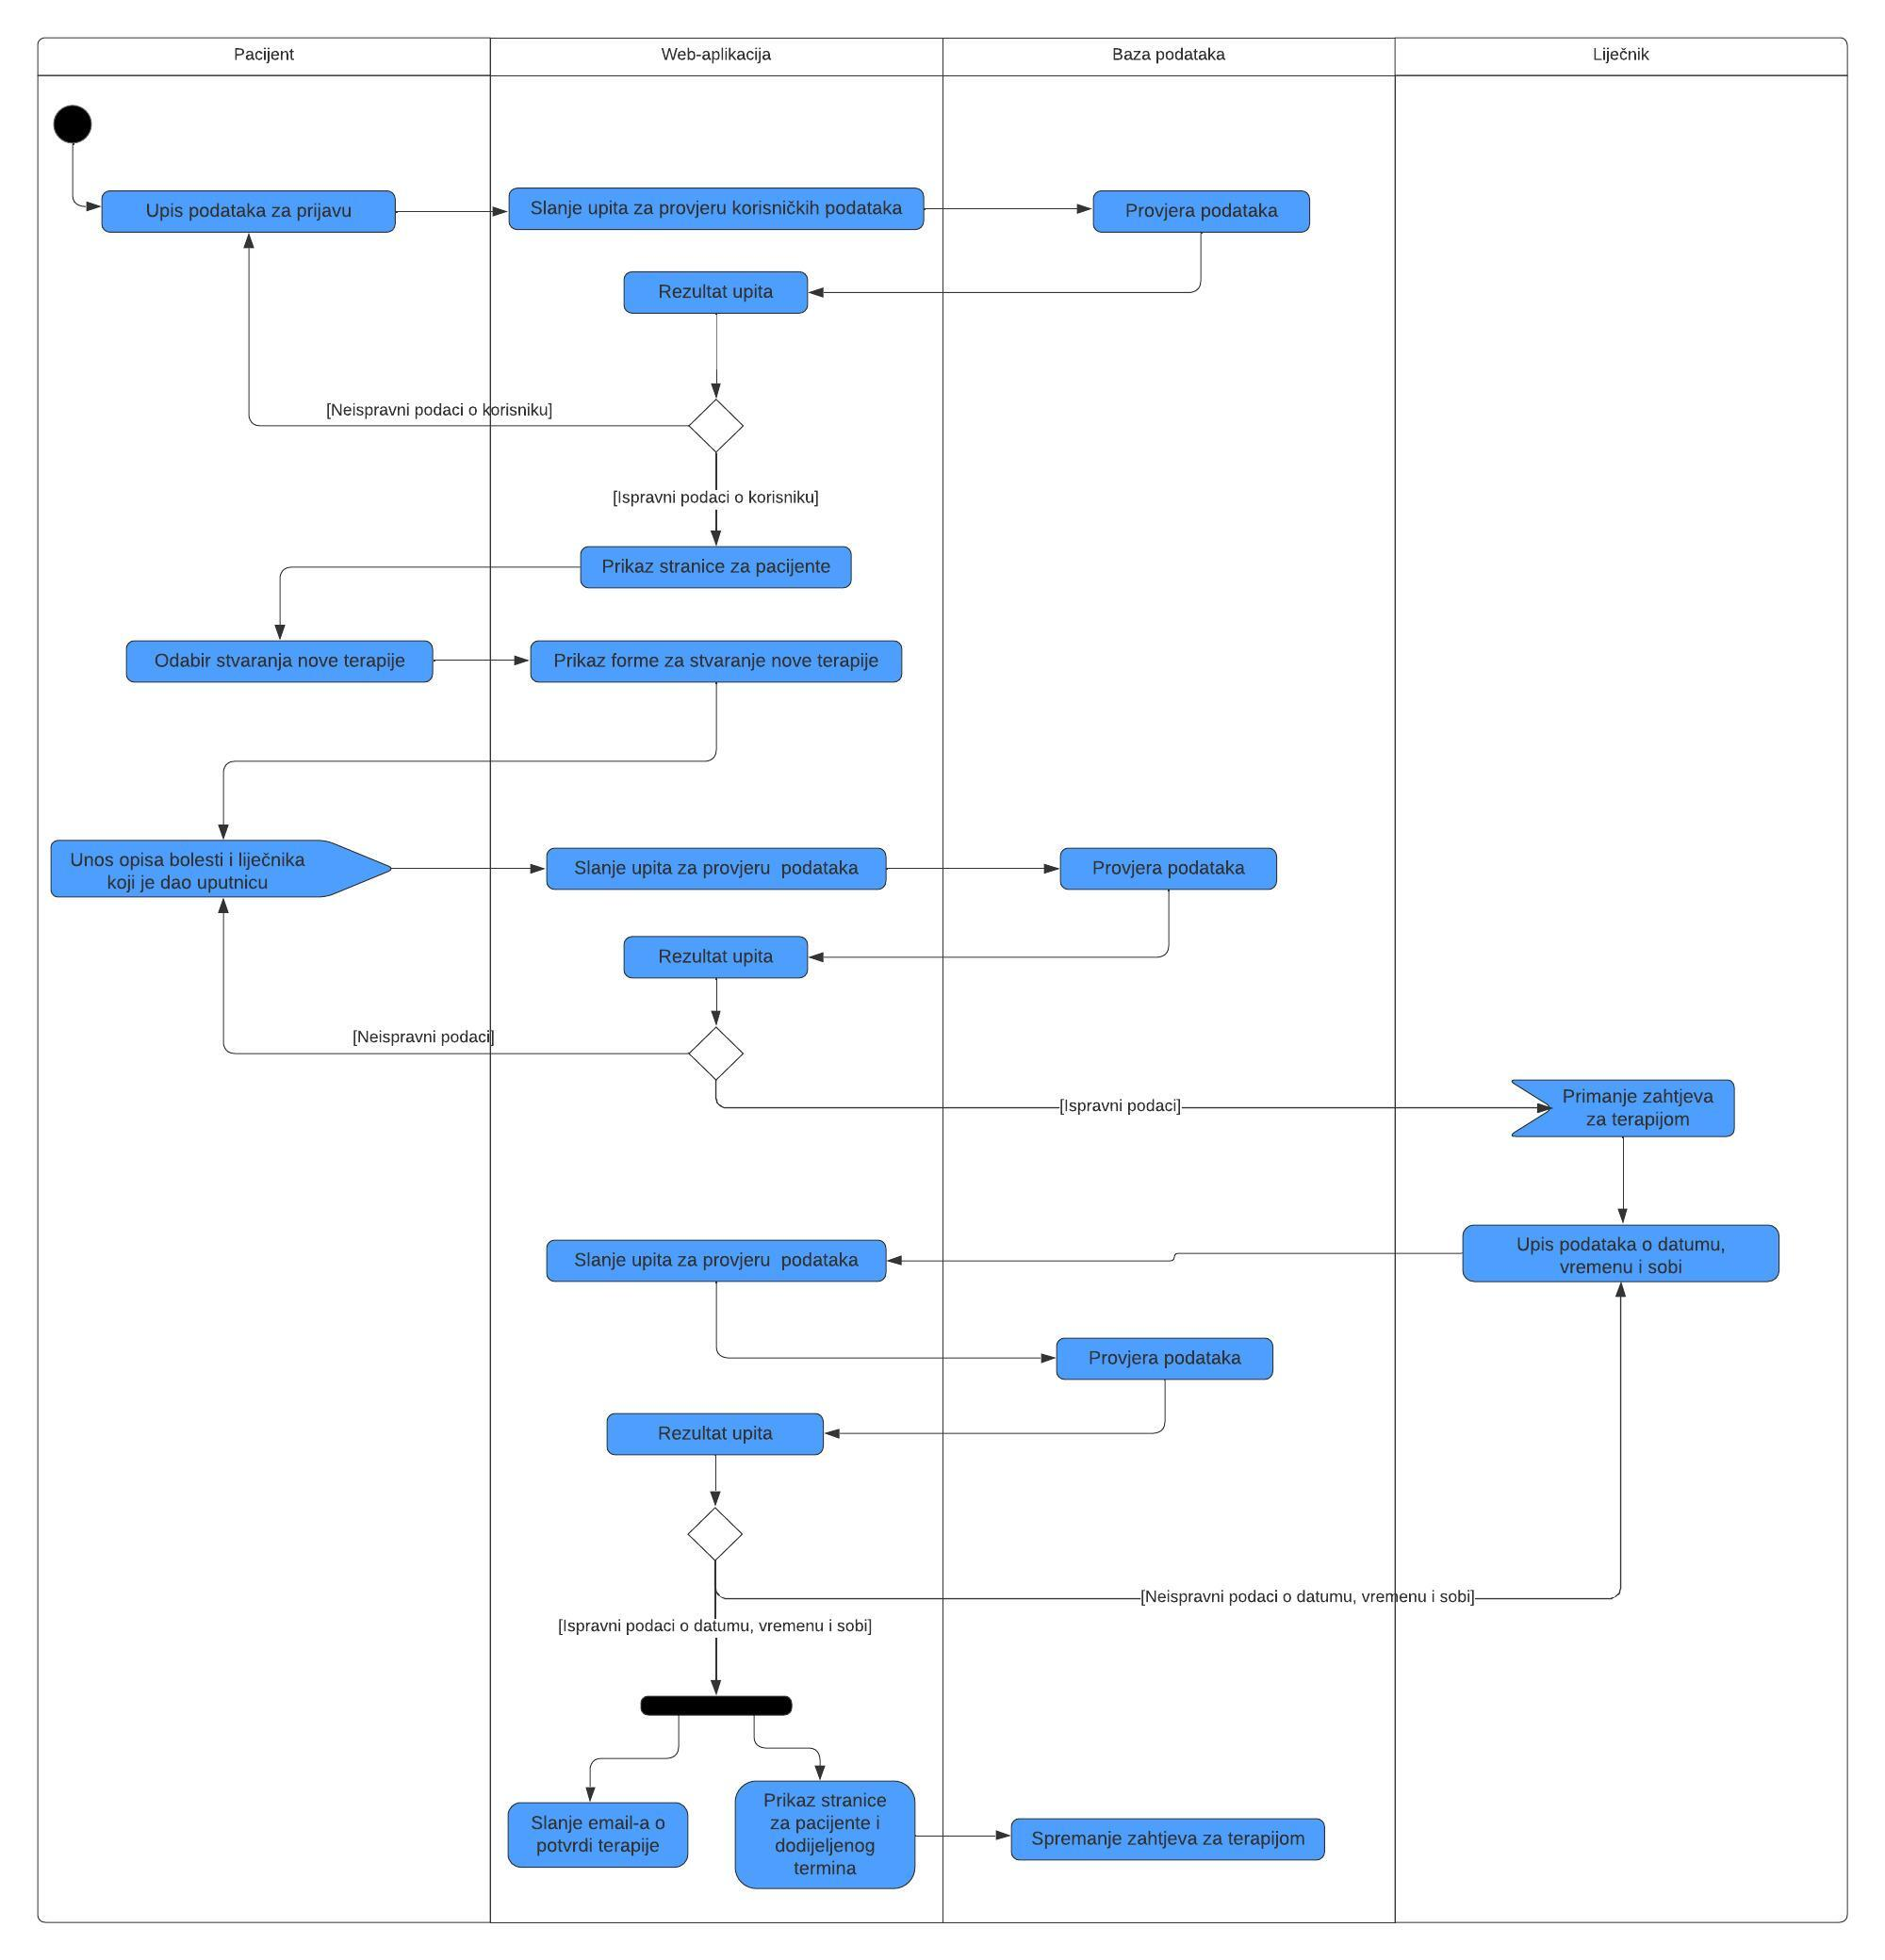
\includegraphics[scale=0.45]{dijagrami/Activity diagram.jpeg}
	\centering
	\caption{Dijagram aktivnosti}
	\label{fig:ActivityDiagram}
\end{figure}

\eject
\section{Dijagram komponenti}

Dijagram komponenti detaljno opisuje strukturu sustava, međusobne veze između komponenti te njihove odnose s okolinom. Prikazuje integraciju frontend i backend aplikacija putem REST API-ja. Backend aplikacija je složena od servisa, repozitorija i kontrolera. Repozitorij komunicira s bazom podataka putem SQL upita kako bi dohvatio potrebne podatke. Servis komunicira s repozitorijem i kontrolerom. Kontroler obrađuje dolazne zahtjeve s frontenda. Frontend aplikacija obuhvaća routere, komponente, servise te razne biblioteke. Router je komponenta koja, na temelju korisničkog zahtjeva za određeni URL, određuje koja datoteka (stranica) će biti isporučena. Komponente predstavljaju stranice koje se isporučuju kao JavaScript datoteke (HTML, CSS, JavaScript kod) ovisne o React biblioteci. Servisi imaju ulogu zahtjeva prema backendu, validacije i sličnih zadataka. Axios, kao biblioteka HTTP klijenta, pojednostavljuje slanje HTTP zahtjeva prema REST API-ju, odnosno prema backend aplikaciji.

\begin{figure}[H]
	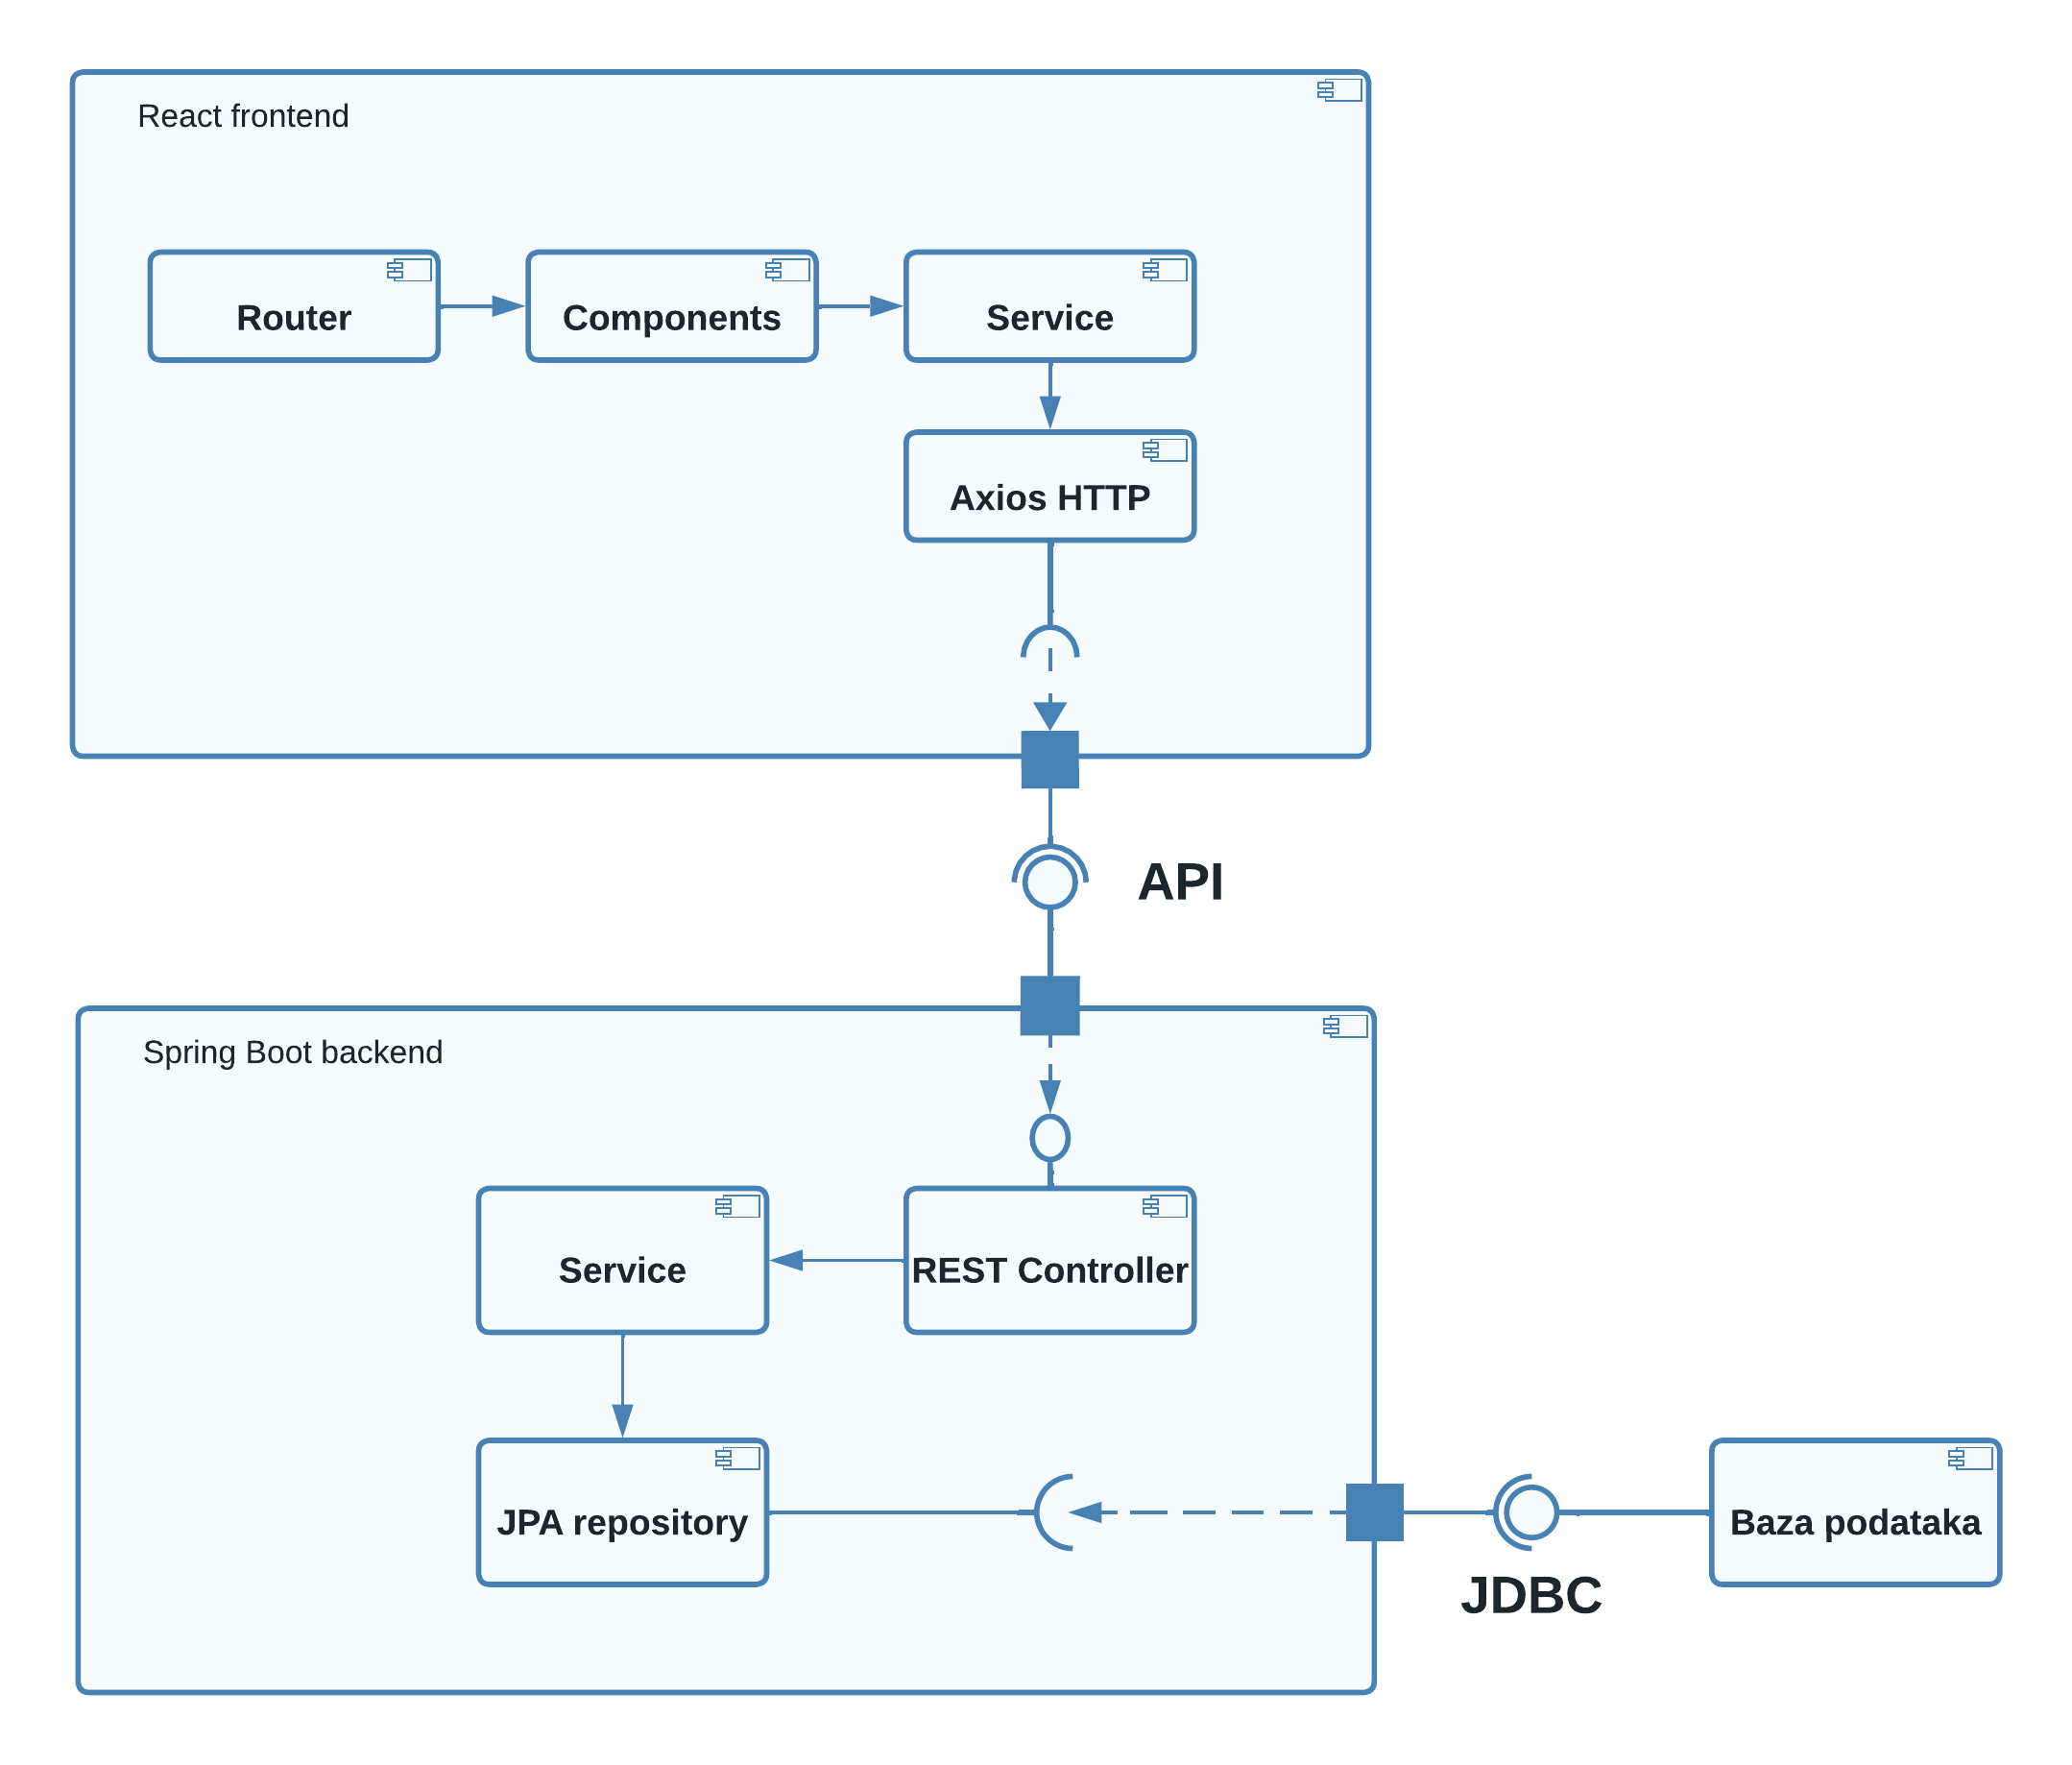
\includegraphics[scale=0.17]{dijagrami/component_diagram.png}
	\centering
	\caption{Dijagram komponenti}
	\label{fig:component_diagram}
\end{figure}
	\chapter{Implementacija i korisničko sučelje}
		
		
		\section{Korištene tehnologije i alati}
		
			Frontend aplikacije realiziran je pomoću \href{https://reactjs.org}{Reacta} korištenjem programskog jezika \href{https://www.javascript.com/}{Javascript}.  React je Javascript biblioteka otvorenog koda za izgradnju korisničkih sučelja temeljenih na komponentama korisničkog sučelja. Backend aplikacije ostvaren je pomoću \href{https://spring.io/projects/spring-boot/}{Spring Boota} zasnovanog na razvojnom okviru \href{https://spring.io}{Spring}, pisanog u programskom jeziku \href{https://www.java.com/en/}{Java}. Od razvojnih okolina korišteni su \href{https://code.visualstudio.com/}{Visual Studio Code} i \href{https://www.jetbrains.com/idea/}{IntelliJ IDEA}. Pri uspostavi arhitekture su također korišteni \href{https://render.com/}{Render}, \href{https://www.netlify.com/}{Netlify}, \href{https://tailwindcss.com/}{Tailwind CSS}, \href{https://docs.docker.com}{Docker Docs}, \href{https://axios-http.com/}{Axios}, \href{https://reactrouter.com/en/main}{React-Router-Dom} i \href{https://www.google.com/recaptcha/}{reCAPTCHA}. Baza podataka pisana je u \href{https://www.postgresql.org/}{PostgreSQL}. Za komunikaciju, dogovore i sastanke korišteni su \href{https://web.whatsapp.com/}{WhatsApp}, \href{https://www.microsoft.com/en-us/microsoft-teams/log-in}{Microsoft Teams} te \href{https://start.atlassian.com/}{Atlassian}. \href{https://www.lucidchart.com/pages/}{Lucidchart} je alat korišten za kreiranje dijagrama, a sama dokumentacija je pisana u markup jeziku \href{https://www.latex-project.org}{LaTeX} te uz pomoć alata \href{https://www.overleaf.com/}{Overleaf}. Udaljeni repozitorij projekta smješten je na web platformi \href{https://github.com/}{GitHub}.
			
			
			\eject 
		
	
		\section{Ispitivanje programskog rješenja}
			
			\textbf{\textit{dio 2. revizije}}\\
			
			 \textit{U ovom poglavlju je potrebno opisati provedbu ispitivanja implementiranih funkcionalnosti na razini komponenti i na razini cijelog sustava s prikazom odabranih ispitnih slučajeva. Studenti trebaju ispitati temeljnu funkcionalnost i rubne uvjete.}
	
			
			\subsection{Ispitivanje komponenti}
			\textit{Potrebno je provesti ispitivanje jedinica (engl. unit testing) nad razredima koji implementiraju temeljne funkcionalnosti. Razraditi \textbf{minimalno 6 ispitnih slučajeva} u kojima će se ispitati redovni slučajevi, rubni uvjeti te izazivanje pogreške (engl. exception throwing). Poželjno je stvoriti i ispitni slučaj koji koristi funkcionalnosti koje nisu implementirane. Potrebno je priložiti izvorni kôd svih ispitnih slučajeva te prikaz rezultata izvođenja ispita u razvojnom okruženju (prolaz/pad ispita). }
			
			
			
			\subsection{Ispitivanje sustava}
			
			 \textit{Potrebno je provesti i opisati ispitivanje sustava koristeći radni okvir Selenium\footnote{\url{https://www.seleniumhq.org/}}. Razraditi \textbf{minimalno 4 ispitna slučaja} u kojima će se ispitati redovni slučajevi, rubni uvjeti te poziv funkcionalnosti koja nije implementirana/izaziva pogrešku kako bi se vidjelo na koji način sustav reagira kada nešto nije u potpunosti ostvareno. Ispitni slučaj se treba sastojati od ulaza (npr. korisničko ime i lozinka), očekivanog izlaza ili rezultata, koraka ispitivanja i dobivenog izlaza ili rezultata.\\ }
			 
			 \textit{Izradu ispitnih slučajeva pomoću radnog okvira Selenium moguće je provesti pomoću jednog od sljedeća dva alata:}
			 \begin{itemize}
			 	\item \textit{dodatak za preglednik \textbf{Selenium IDE} - snimanje korisnikovih akcija radi automatskog ponavljanja ispita	}
			 	\item \textit{\textbf{Selenium WebDriver} - podrška za pisanje ispita u jezicima Java, C\#, PHP koristeći posebno programsko sučelje.}
			 \end{itemize}
		 	\textit{Detalji o korištenju alata Selenium bit će prikazani na posebnom predavanju tijekom semestra.}
			
			\eject 
		
		
		\section{Dijagram razmještaja}
			
			Dijagram razmještaja opisuje strukturu sustava, tj. odnose između sklopovskih i programskih dijelova. Donja slika predstavlja specifikacijski dijagram razmještaja, pri čemu se na poslužiteljskom računalu nalaze web aplikacija i baza podataka. Pristup aplikaciji klijenti ostvaruju putem web preglednika. Funkcioniranje sustava temelji se na modelu "klijent - poslužitelj", gdje klijenti zahtijevaju usluge od poslužitelja putem HTTP zahtjeva te očekuju odgovor. Poslužitelj obrađuje zahtjeve i šalje odgovore klijentima, a istovremeno upravlja komunikacijom s bazom podataka.

            \begin{figure}[H]
			         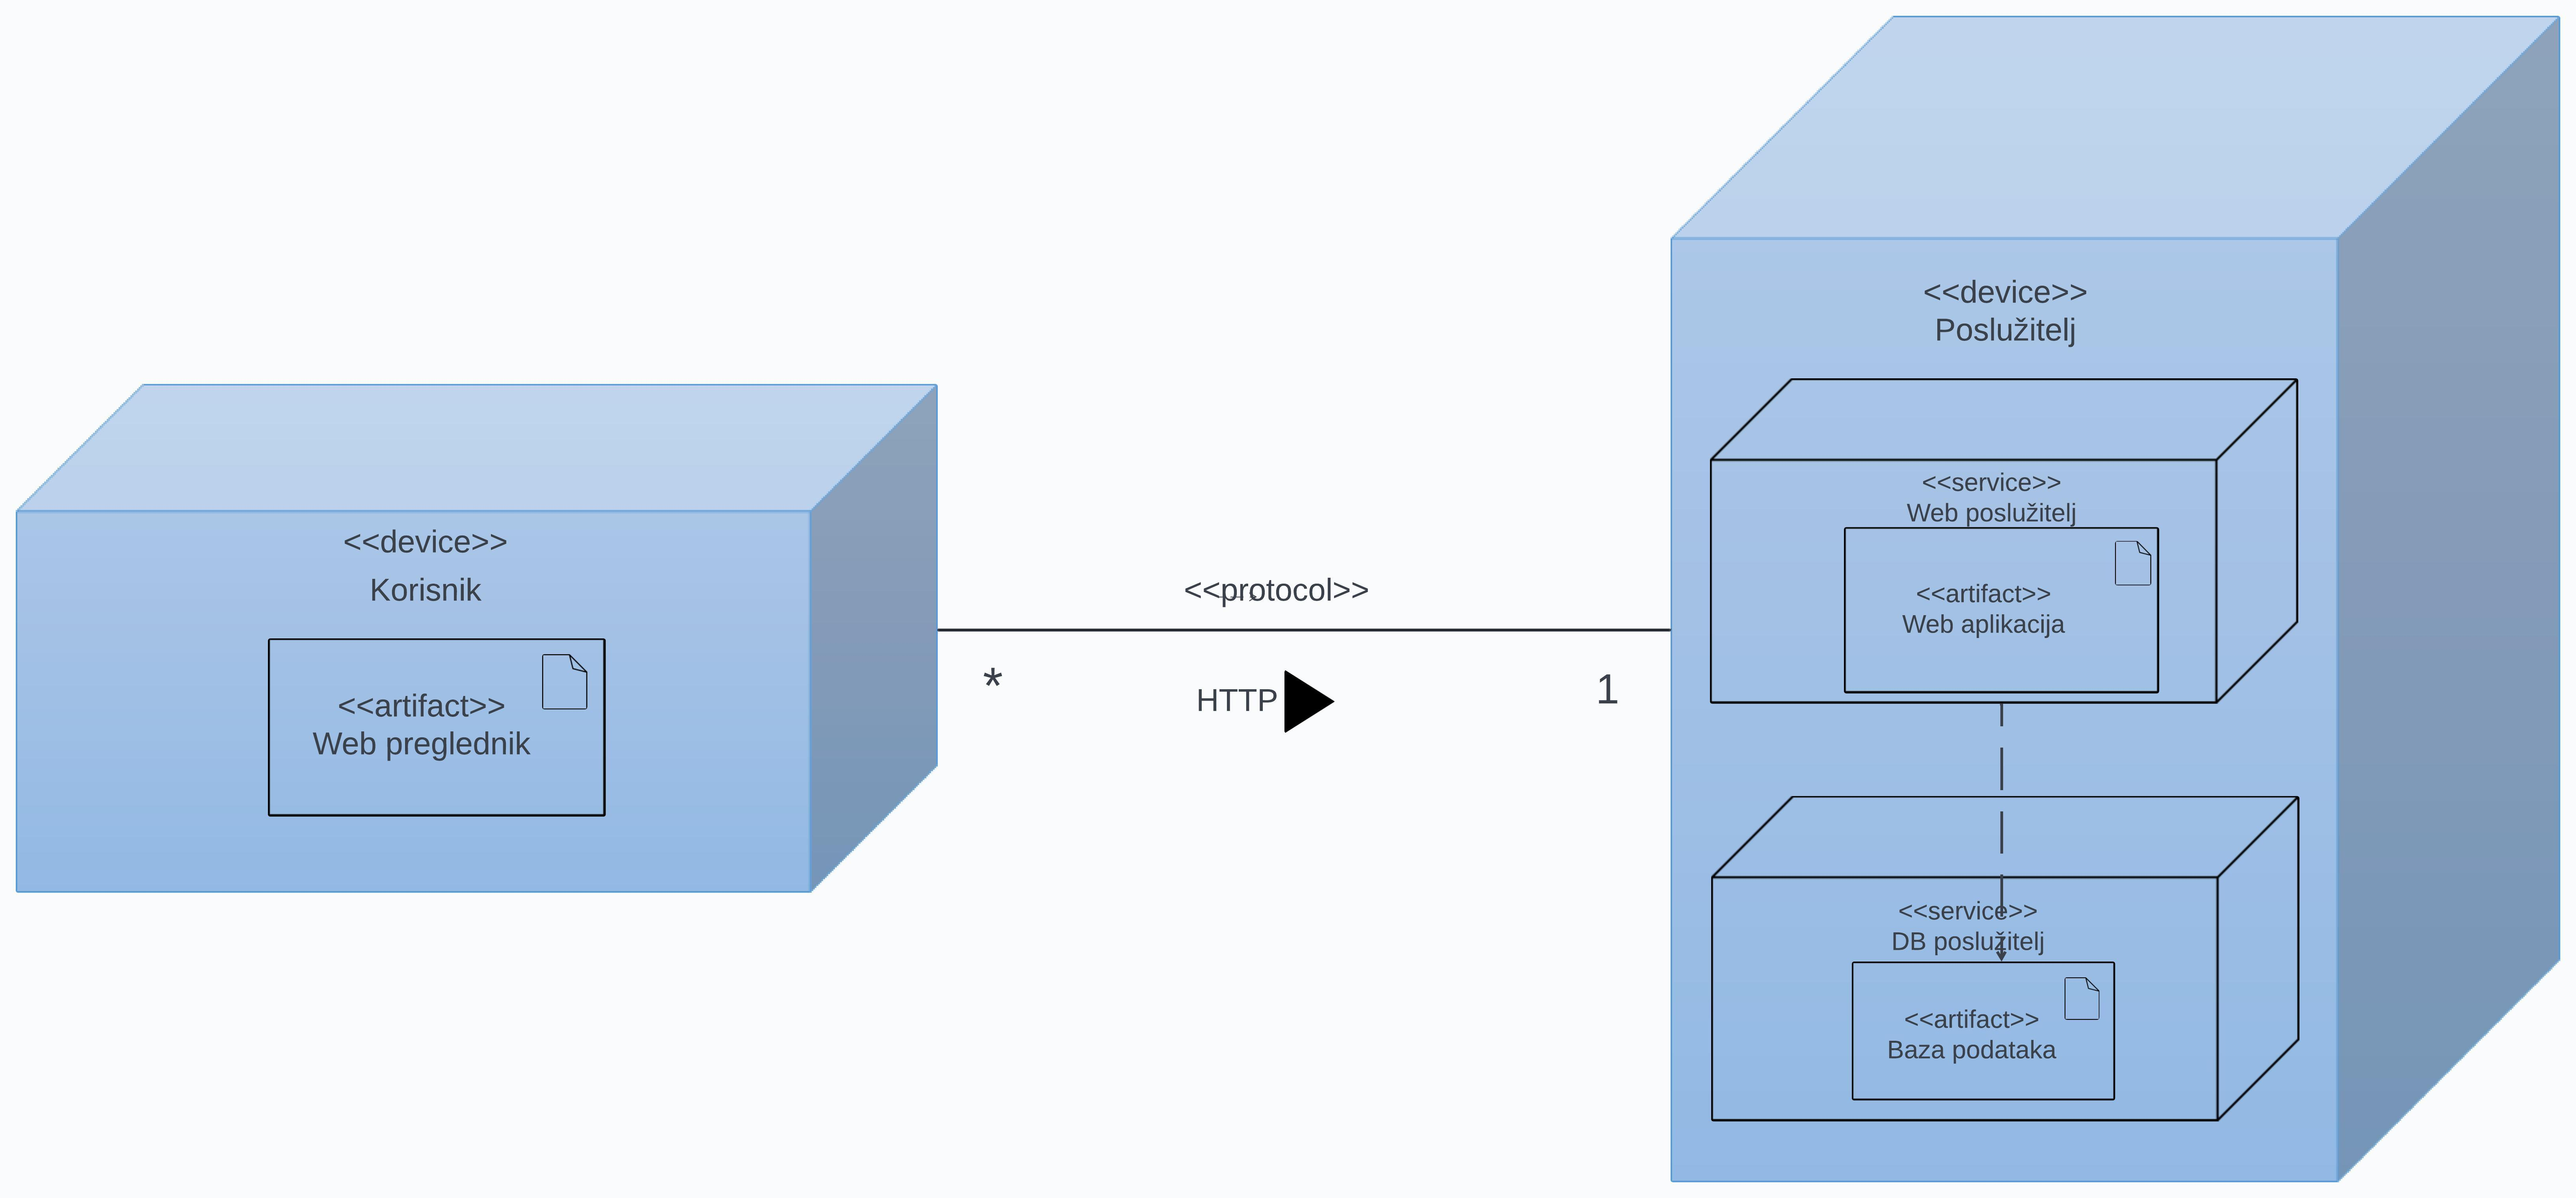
\includegraphics[scale=0.15]{dijagrami/Layout Diagram.jpeg}
			         \centering
			         \caption{Specifikacijski dijagram razmještaja}
			         \label{fig:LayoutDiagram}
		    \end{figure}
			
			\eject 
		
		\section{Upute za puštanje u pogon}
		
			\textbf{\textit{dio 2. revizije}}\\
		
			 \textit{U ovom poglavlju potrebno je dati upute za puštanje u pogon (engl. deployment) ostvarene aplikacije. Na primjer, za web aplikacije, opisati postupak kojim se od izvornog kôda dolazi do potpuno postavljene baze podataka i poslužitelja koji odgovara na upite korisnika. Za mobilnu aplikaciju, postupak kojim se aplikacija izgradi, te postavi na neku od trgovina. Za stolnu (engl. desktop) aplikaciju, postupak kojim se aplikacija instalira na računalo. Ukoliko mobilne i stolne aplikacije komuniciraju s poslužiteljem i/ili bazom podataka, opisati i postupak njihovog postavljanja. Pri izradi uputa preporučuje se \textbf{naglasiti korake instalacije uporabom natuknica} te koristiti što je više moguće \textbf{slike ekrana} (engl. screenshots) kako bi upute bile jasne i jednostavne za slijediti.}
			
			
			 \textit{Dovršenu aplikaciju potrebno je pokrenuti na javno dostupnom poslužitelju. Studentima se preporuča korištenje neke od sljedećih besplatnih usluga: \href{https://aws.amazon.com/}{Amazon AWS}, \href{https://azure.microsoft.com/en-us/}{Microsoft Azure} ili \href{https://www.heroku.com/}{Heroku}. Mobilne aplikacije trebaju biti objavljene na F-Droid, Google Play ili Amazon App trgovini.}
			
			
			\eject 
	\chapter{Zaključak i budući rad}
		
		Suočili smo se s izazovom razvoja web aplikacije za naručivanje medicinske rehabilitacije. Vrijednost koju smo najviše cijenili bila je suradnja u timu, koja je donijela raznolike izazove s kojima smo se uspješno nosili. Voditelj grupe imao je zahtjevan zadatak koordinacije sedmero ljudi, što nije bilo jednostavno. Početni susret s mnogim novim konceptima zahtijevao je brzo učenje i intenzivan rad na aplikaciji i dokumentaciji.

        Razumijevanje alata i tehnologija korištenih u izradi aplikacije i dokumentacije predstavljalo je dodatan izazov koji je zahtijevao značajan vremenski angažman. S vremenom proces je postao olakšan jer smo se bolje prilagodili timskom radu i aktivno si pružali podršku. Iako smo uvjereni da bi aplikacija mogla ostvariti još veći napredak s više vremena na raspolaganju, zadovoljni smo končanim rezultatom s obzirom na fakultetske i druge obaveze svakog člana tima.

        Prijedlozi za budući rad obuhvaćaju proširenje funkcionalnosti aplikacije, kao što su dodatne opcije za korisnike, poboljšane analize statistike rehabilitacije te implementacija dodatnih sigurnosnih slojeva. Također, istraživanje mogućnosti integracije novih tehnologija i prilagodba sučelja prema povratnim informacijama korisnika predstavljaju ključne smjernice za daljnji razvoj "ReHub" aplikacije.

        Kvalitetna komunikacija među članovima tima bila je ključna. Koristili smo alate poput WhatsAppa, Teamsa i Atlassian platforme. Redovito održavani sastanci služili su za raspravu o zadacima, pregled dosadašnjeg rada te dodjeljivanje novih zadataka. Sastanci su se održavali prema potrebi. 
        
        Na kraju, prepoznali smo da su opuštena atmosfera, međusobna pomoć i organizirano vođenje od strane voditelja ključni faktori za postizanje krajnjeg cilja.
        		
		\eject 
	\chapter*{Popis literature}
\addcontentsline{toc}{chapter}{Popis literature}



\begin{enumerate}
	
	
	\item  Programsko inženjerstvo, FER ZEMRIS, \url{http://www.fer.hr/predmet/proinz}
	
	\item  The Unified Modeling Language, \url{https://www.uml-diagrams.org/}
	
	\item  Astah  Community, \url{http://astah.net/editions/uml-new}
	
	\item  Baeldung, \url{https://www.baeldung.com}
	
	\item  Tehnička predavanja tvrtke Croz, \url{https://gitlab.com/progi-deploy-demo}
	
	\item  React tutorial, \url{ https://www.w3schools.com/REACT/DEFAULT.ASP}
	
	\item Moodle - Programsko inženjertsvo, \url{https://moodle.fer.hr/course/view.php?id=527}
\end{enumerate}


	
	
	\begingroup
	\renewcommand*\listfigurename{Indeks slika i dijagrama}
	%\renewcommand*\listtablename{Indeks tablica}
	%\let\clearpage\relax
	\listoffigures
	%\vspace{10mm}
	%\listoftables
	\endgroup
	\addcontentsline{toc}{chapter}{Indeks slika i dijagrama}


	
	\eject 
		
	\chapter*{Dodatak: Prikaz aktivnosti grupe}
		\addcontentsline{toc}{chapter}{Dodatak: Prikaz aktivnosti grupe}
		
		\section*{Dnevnik sastajanja}
		
		
		\begin{packed_enum}
			\item  sastanak
			
			\item[] \begin{packed_item}
				\item Datum: 16. listopada 2023.
				\item Prisustvovali: Kašik, Begić, Vivoda, Greblo, Miletić
				\item Teme sastanka:
				\begin{packed_item}
					\item  Upoznavanje s kolegama
				\end{packed_item}
			\end{packed_item}
			
			\item  sastanak
			\item[] \begin{packed_item}
				\item Datum: 18. listopada 2023.
				\item Prisustvovali: Kašik, Begić, Krstičević, Mikulić, Vivoda, Greblo, Miletić
				\item Teme sastanka:
				\begin{packed_item}
					\item  Upoznavanje s projektnim zadatkom
					\item  Podjela zadataka
                    \item  Dogovor oko načina daljnje komunikacije
				\end{packed_item}
			\end{packed_item}

            \item  sastanak
			\item[] \begin{packed_item}
				\item Datum: 19. listopada 2023.
				\item Prisustvovali: Kašik, Krstičević
				\item Teme sastanka:
				\begin{packed_item}
					\item  Dogovor oko daljnje raspodjele posla
				\end{packed_item}
			\end{packed_item}

            \item  sastanak
			\item[] \begin{packed_item}
				\item Datum: 19. listopada 2023.
				\item Prisustvovali: Begić, Greblo, Vivoda 
				\item Teme sastanka:
				\begin{packed_item}
					\item  Dogovor oko daljnje raspodjele posla
				\end{packed_item}
			\end{packed_item}

            \item  sastanak
			\item[] \begin{packed_item}
				\item Datum: 23. listopada 2023.
				\item Prisustvovali: Kašik, Krstičević
				\item Teme sastanka:
				\begin{packed_item}
					\item  Dogovor oko daljnje raspodjele posla
				\end{packed_item}
			\end{packed_item}

            \item  sastanak
			\item[] \begin{packed_item}
				\item Datum: 24. listopada 2023.
				\item Prisustvovali: Begić, Mikulić, Vivoda, Greblo, Miletić
				\item Teme sastanka:
				\begin{packed_item}
					\item  Dogovor oko daljnje raspodjele posla
				\end{packed_item}
			\end{packed_item}

            \item  sastanak
			\item[] \begin{packed_item}
				\item Datum: 25. listopada 2023.
				\item Prisustvovali: Kašik, Begić 
				\item Teme sastanka:
				\begin{packed_item}
					\item  Laboratorijska vježba
				\end{packed_item}
			\end{packed_item}

            \item  sastanak
			\item[] \begin{packed_item}
				\item Datum: 26. listopada 2023.
				\item Prisustvovali: Kašik, Begić, Krstičević, Mikulić, Vivoda, Greblo, Miletić
				\item Teme sastanka:
				\begin{packed_item}
					\item  Upoznavanje s pokretanjem backenda
                    \item  Predstavljanje dizajna aplikacije
				\end{packed_item}
			\end{packed_item}

            \item  sastanak
			\item[] \begin{packed_item}
				\item Datum: 30. listopada 2023.
				\item Prisustvovali: Kašik, Krstičević
				\item Teme sastanka:
				\begin{packed_item}
					\item  Dogovor oko daljnje raspodjele posla
				\end{packed_item}
			\end{packed_item}

            \item  sastanak
			\item[] \begin{packed_item}
				\item Datum: 31. listopada 2023.
				\item Prisustvovali: Begić, Mikulić, Vivoda, Greblo, Miletić
				\item Teme sastanka:
				\begin{packed_item}
					\item  Dogovor oko daljnje raspodjele posla
				\end{packed_item}
			\end{packed_item}

            \item  sastanak
			\item[] \begin{packed_item}
				\item Datum: 6. studeni 2023.
				\item Prisustvovali: Kašik, Krstičević
				\item Teme sastanka:
				\begin{packed_item}
					\item  Dogovor oko daljnje raspodjele posla
				\end{packed_item}
			\end{packed_item}

            \item  sastanak
			\item[] \begin{packed_item}
				\item Datum: 7. studeni 2023.
				\item Prisustvovali: Begić, Mikulić, Vivoda, Greblo, Miletić
				\item Teme sastanka:
				\begin{packed_item}
					\item  Dogovor oko daljnje raspodjele posla
				\end{packed_item}
			\end{packed_item}

            \item  sastanak
			\item[] \begin{packed_item}
				\item Datum: 8. studeni 2023.
				\item Prisustvovali: Kašik, Begić, Krstičević, Mikulić, Vivoda, Greblo, Miletić
				\item Teme sastanka:
				\begin{packed_item}
					\item  Dogovor oko daljnje raspodjele posla
                    \item  Dogovor vezan uz izradu dokumentacije
                    \item  Laboratorijska vježba
				\end{packed_item}
			\end{packed_item}

            \item  sastanak
			\item[] \begin{packed_item}
				\item Datum: 13. studeni 2023.
				\item Prisustvovali: Kašik, Krstičević
				\item Teme sastanka:
				\begin{packed_item}
					\item  Dogovor oko daljnje raspodjele posla
				\end{packed_item}
			\end{packed_item}

            \item  sastanak
			\item[] \begin{packed_item}
				\item Datum: 14. studeni 2023.
				\item Prisustvovali: Begić, Mikulić, Vivoda, Greblo, Miletić
				\item Teme sastanka:
				\begin{packed_item}
					\item  Dogovor oko daljnje raspodjele posla
				\end{packed_item}
			\end{packed_item}

            \item  sastanak
			\item[] \begin{packed_item}
				\item Datum: 15. studeni 2023.
				\item Prisustvovali: Kašik, Begić, Krstičević, Mikulić, Vivoda, Greblo, Miletić
				\item Teme sastanka:
				\begin{packed_item}
					\item  Dogovor oko daljnje raspodjele posla
                    \item  Završni pregled dosad napravljenog posla
				\end{packed_item}
			\end{packed_item}

            \item  sastanak
			\item[] \begin{packed_item}
				\item Datum: 6. prosinac 2023.
				\item Prisustvovali: Kašik, Begić, Krstičević, Mikulić, Vivoda, Greblo, Miletić
				\item Teme sastanka:
				\begin{packed_item}
                    \item  Laboratorijska vježba
				\end{packed_item}
			\end{packed_item}

            \item  sastanak
			\item[] \begin{packed_item}
				\item Datum: 11. prosinac 2023.
				\item Prisustvovali: Kašik, Begić, Krstičević, Mikulić, Vivoda, Greblo, Miletić
				\item Teme sastanka:
				\begin{packed_item}
                    \item  Dogovor oko daljnje raspodjele posla
				\end{packed_item}
			\end{packed_item}

            \item  sastanak
			\item[] \begin{packed_item}
				\item Datum: 18. prosinac 2023.
				\item Prisustvovali: Kašik, Krstičević
				\item Teme sastanka:
				\begin{packed_item}
					\item  Dogovor oko daljnje raspodjele posla
				\end{packed_item}
			\end{packed_item}

            \item  sastanak
			\item[] \begin{packed_item}
				\item Datum: 19. prosinac 2023.
				\item Prisustvovali: Begić, Mikulić, Vivoda, Greblo, Miletić
				\item Teme sastanka:
				\begin{packed_item}
					\item  Dogovor oko daljnje raspodjele posla
				\end{packed_item}
			\end{packed_item}

            \item  sastanak
			\item[] \begin{packed_item}
				\item Datum: 03. siječanj 2024.
				\item Prisustvovali: Kašik, Begić, Krstičević, Mikulić, Vivoda, Greblo, Miletić
				\item Teme sastanka:
				\begin{packed_item}
					\item  Dogovor oko daljnje raspodjele posla
				\end{packed_item}
			\end{packed_item}

            \item  sastanak
			\item[] \begin{packed_item}
				\item Datum: 08. siječanj 2024.
				\item Prisustvovali: Kašik, Krstičević
				\item Teme sastanka:
				\begin{packed_item}
					\item  Dogovor oko daljnje raspodjele posla
				\end{packed_item}
			\end{packed_item}

            \item  sastanak
			\item[] \begin{packed_item}
				\item Datum: 09. siječanj 2024.
				\item Prisustvovali: Begić, Mikulić, Vivoda, Greblo, Miletić
				\item Teme sastanka:
				\begin{packed_item}
					\item  Dogovor oko daljnje raspodjele posla
				\end{packed_item}
			\end{packed_item}

            \item  sastanak
			\item[] \begin{packed_item}
				\item Datum: 10. siječanj 2024.
				\item Prisustvovali: Kašik, Begić, Krstičević, Mikulić, Vivoda, Greblo
				\item Teme sastanka:
				\begin{packed_item}
					\item  Dogovor oko daljnje raspodjele posla
                    \item  Laboratorijska vježba
				\end{packed_item}
			\end{packed_item}

            \item  sastanak
			\item[] \begin{packed_item}
				\item Datum: 18. siječanj 2024.
				\item Prisustvovali: Kašik, Begić, Krstičević, Mikulić, Vivoda, Greblo, Miletić
				\item Teme sastanka:
				\begin{packed_item}
					\item  Završni pregled napravljenog
				\end{packed_item}
			\end{packed_item}
			
			%
			
		\end{packed_enum}
		
		\eject
		\section*{Tablica aktivnosti}
		

			\begin{longtblr}[
					label=none,
				]{
					vlines,hlines,
					width = \textwidth,
					colspec={X[7, l]X[1, c]X[1, c]X[1, c]X[1, c]X[1, c]X[1, c]X[1, c]}, 
					vline{1} = {1}{text=\clap{}},
					hline{1} = {1}{text=\clap{}},
					rowhead = 1,
				} 
			
				\SetCell[c=1]{c}{} & \SetCell[c=1]{c}{\rotatebox{90}{\textbf{Dora Kašik}}} & \SetCell[c=1]{c}{\rotatebox{90}{\textbf{Josip Begić }}} &	\SetCell[c=1]{c}{\rotatebox{90}{\textbf{Roko Krstičević }}} & \SetCell[c=1]{c}{\rotatebox{90}{\textbf{Katarina Mikulić }}} &	\SetCell[c=1]{c}{\rotatebox{90}{\textbf{Anton Vivoda }}} & \SetCell[c=1]{c}{\rotatebox{90}{\textbf{Erik Greblo }}} &	\SetCell[c=1]{c}{\rotatebox{90}{\textbf{Marko Miletić }}} \\  
				Upravljanje projektom 		&6  &5  &  &  &  &  &2 \\ 
				Opis projektnog zadatka 	&  &  &  &  &  &  &7 \\ 
				
				Funkcionalni zahtjevi       &7  &  &  &9  &  &  &  \\ 
				Opis pojedinih obrazaca 	&9  &  &  &6  &  &  &4  \\ 
				Dijagram obrazaca 			&6  &  &  &9  &  &  &3  \\ 
				Sekvencijski dijagrami 		&  &  &5  &  &2  &3  &  \\ 
				Opis ostalih zahtjeva 		&  &2  &5  &  &  &  &  \\ 

				Arhitektura i dizajn sustava	 &4  &  &6  &  &  &  &4  \\ 
				Baza podataka				&  &4  &  &  &3  &5  &   \\ 
				Dijagram razreda 			&  &2  &  &  &3  &  &3   \\ 
				Dijagram stanja				&  &3  &  &  &  &  &4  \\ 
				Dijagram aktivnosti 		&  &  &  &  &4  &2  &3  \\ 
				Dijagram komponenti			&  &  &3  &  &4  &  &  \\ 
				Korištene tehnologije i alati 		&  &  &5  &  &  &  &  \\ 
				Ispitivanje programskog rješenja 	&  &  &6  &  &  &  &  \\ 
				Dijagram razmještaja			&  &  &  &  &  &  &3  \\ 
				Upute za puštanje u pogon 		&  &  &5  &  &  &  &  \\  
				Dnevnik sastajanja 			&  &  &  &  &  &  &1  \\ 
				Zaključak i budući rad 		&  &  &  &  &  &  &1  \\  
				Popis literature 			&  &  &  &  &  &  &1  \\  
				&  &  &  &  &  &  &  \\ \hline 
				\textit{izrada plana stranica} 				&5  &  &  &  &  &  &  \\  
				\textit{back end} 							&  &23  &  &11  &19  &25  &  \\  
				 							&  &  &  &  &  &  &\\ 
			\end{longtblr}
					
					
		\eject
		\section*{Dijagrami pregleda promjena}
		
		\textbf{\textit{dio 2. revizije}}\\
		
		\textit{Prenijeti dijagram pregleda promjena nad datotekama projekta. Potrebno je na kraju projekta generirane grafove s gitlaba prenijeti u ovo poglavlje dokumentacije. Dijagrami za vlastiti projekt se mogu preuzeti s gitlab.com stranice, u izborniku Repository, pritiskom na stavku Contributors.}
		
	


\end{document} %naredbe i tekst nakon ove naredbe ne ulaze u izgrađen dokument 


